\section{Automatic Narrative Elicitation}
\label{cha:methodology-personal-narrative-elicitation-results}
% HUMAN EVAL Comprono le guidelnies, ma non sono speicifche
% LA HUMAN EVAL è UNA BUONA PROXY, study of better metrics
% exactly measure empathy/guidelines compliance/
% perchè le mtriche sono fighe ? 
After the previous selection procedure, we were left with models that are able to answer in Italian, with reasonable story closure abilities, in particular for ChatGPT 3-5 and 4.

In this section, an analysis of the results obtained in the successive ANE task is conducted. This analysis is conducted with different automatic metrics and, as a marked difference from the previous experiments using \emph{Story Cloze Test}, a comparison of the LLM-generated data with the crowdsourced data is also made.

\begin{table}[!htbp]
\centering
\caption{Two examples of narratives and model outputs for different experimental settings are shown in each of the two rows. To evaluate the models, their outputs are processed by removing special invalid characters and only the first sentence, marked by the dot (\emph{?}), is considered. In the middle, it is possible to read the raw unprocessed model output, which is unsuitable for our task. Therefore some post-processing operations are automatically applied in order to extract a better elicitation, which is reported in the second rightmost column. On the rightmost column the human crowdsourced eliciting question for the same narrative as reference. }
\label{tab:personal-narrative-elicitation-example-answers}
    \centering
    \begin{tabularx}{\linewidth}{p{2.5cm}| p{1.5cm} | p{2cm} | X | p{2cm} | p{2cm} }
    % \begin{tabular}{p{1.5cm}|p{3cm}|p{5cm}|p{2.5cm}|p{2cm}}
        \toprule
        \thead{Experimental \\ Setting} & \thead{Model \\ name} & \thead{Narrative} & \thead{Unprocessed \\Model \\ eliciting question}& \thead{Processed \\ Model \\eliciting question} & \thead{Human \\ eliciting question} \\
        \midrule
\textbf{0-shot without guidelines without colour} & Mpt 7B & Oggi sono molto più tranquilla . . . fine settimana gratificante in famiglia. Era il mio compleanno e finalmente avevo tutta la mia famiglia riunita.  &  Perché la tua vita è molto più tranquilla oggi? Risposta: 'Domani ho un esame. ' 'Domani mi è stato detto che la mia madre mi sta cercando, ma non è più la mia città.' 'Domani ho un prossimo di casa. ' 'Domani è la mia festa. ' 'Domani è l'anno nuovo e tutta la mia famiglia è qui. ' 'Domani devo pagare il mio bollo. ' 'Domani sono le vacanze. ' 'Domani sono i miei amici. ' 'Domani sono il mare. ' 'Domani sono le mie amiche. ' 'Domani sono le mie scuole. ' 'Domani sono le mie parole. ' 'Domani sono le mie gioie. ' 'Domani sono le mie parole...' & Perché la tua vita è molto più tranquilla oggi? & Mi fa piacere sentirlo, come avete celebrato? \\
\midrule
\textbf{5-shot with guidelines without colour} &  Vicuna 33B V1  & Ritornata dal lavoro mia figlia mi dice di aver chiamato il medico perché ha dei dolori alla testa non ha il senso dell'olfatto e del gusto per cui ci siamo un po' allarmati. & 1. Quali altri segni o sintomi ha segnato la tua figlia oltre al mal di testa, alla perdita del senso dell'olfatto e del gusto? 2. In quale momento della giornata ha chiamato il medico e quali esami o accertamenti ha richiesto? 3. Quali sono le tue preoccupazioni in merito a queste condizioni della tua figlia? 4. È stata presa alcuna decision & Quali altri segni o sintomi ha segnato la tua figlia oltre al mal di testa, alla perdita del senso dell'olfatto e del gusto? &Mi dispiace di sentirlo, da quanto tempo tua figlia ha questi sintomi? \\
        \bottomrule
    \end{tabularx}
\end{table}

Looking at the eliciting questions produced by the models, it is possible to witness that the problem of the answers of the model containing special non-text characters is still present, as shown in Table \ref{tab:personal-narrative-elicitation-example-answers}. The same behaviour of degeneration in the quality of the text is also present. Therefore, a similar pattern to the previous experiments was applied in order to retrieve the responses of the models, with the difference of using \emph{``?"} instead of \emph{``."} as a sentence delimitator mark. This difference is motivated by the fact that for the ANE task, the models are tasked to produced questions.
% 
\begin{center}
\label{tab:personal-narrative-elicitation-answers}
\begin{longtable}{l|l|l|p{3cm}|p{8cm}}
\caption{Model answers for each of the experimental setup. Notice that most 0 shot results are unusable and they get better with the number of shots and presence of guidelines. Notice how colour information negatively affects the models' responses. } \\ 
\toprule
\multicolumn{2}{l}{\thead{Narrative}} & \multicolumn{3}{}{Oggi sono molto più tranquilla . . . fine settimana gratificante in famiglia. Era il mio compleanno e finalmente avevo tutta la mia famiglia riunita}
\multicolumn{2}{l}{\thead{Human eliciting question}} & \multicolumn{3}{l}{Mi fa piacere sentirlo, come avete celebrato?}
\midrule
 \thead{Colour}& \thead{Guidelines} & \thead{Shot} & \thead{Model name} & \thead{Model eliciting question} \\
\midrule
\multirow[c]{70}{*}{\thead{Without Colour}} & \multirow[c]{36}{*}{\thead{Without Guidelines}} & \multirow[c]{9}{*}{0-shot} & Falcon 7B & Oggi era il compleanno. Quali presentimenti avevi prima del tuo compleanno? \\
 &  &  & Falcon 40B Instruct & Mi puoi dire di più sul compleanno della protagonista del racconto e quali attività hanno svolto la famiglia in quel fine settimana? \\
 &  &  & ChatGPT 3.5 turbo & Che tipo di attività hai svolto con la tua famiglia durante il tuo compleanno? \\
 &  &  & ChatGPT 4 & Come hai festeggiato il tuo compleanno con la tua famiglia? \\
 &  &  & Mpt 7B & Perché la tua vita è molto più tranquilla oggi? \\
 &  &  & Mpt 30B Chat & Cosa ti ha regalato la tua famiglia per il tuo compleanno? \\
 &  &  & Vicuna 13B V1 &  Cè un modo in cui mi potresti chiedere se vuoi ottenere ulteriori informazioni sulla tua esperienza di compleanno? \\
 &  &  & Vicuna 33B V1 &  Quali attività hanno organizzato per festeggiare il compleanno della protagonista? \\
 &  &  & Wizard Vicuna 13B Uncensored HF & Quali eventi accaddero durante il fine settimana che fecero del tuo compleanno una gratificante" esperienza per te? \\
\cline{3-5}
 &  & \multirow[c]{9}{*}{1-shot} & Falcon 7B & Mi piacerebbe sapere se siete andati tutti insieme in vacanza o se cè stato qualcuno in più. "NARRATIVA: 'Oggi è stato un giorno bellissimo. I miei figli hanno organizzato una festa di compleanno per me. Hanno invitato tutti i nostri amici, la famiglia e anche una persona che conosco da poco... "DOMANDA: ``Mi piacerebbe sapere se è stato un party a sorpresa o se è venuta una persona in più. "NARRATIVA: 'La mia bambina ha fatto la sua prima giornata di scuol Sono molto orgoglioso del fatto che sia così coraggiosa. Mi ha anche detto di avere imparato molte cose. 'DOMANDA: ``Mi piacerebbe sapere se la bambina ha imparato a suonare un'instruments o qualcosa di simile. "NARRATIVA: ``Il tempo è stato splendido stamattina. Mi sono alzato presto e ho fatto un giro in bicicletta. 'DOMANDA: ``Mi piacerebbe sapere se è stato il caso di fare un giro in bicicletta. " A questo punto, è possibile procedere come si è visto nel capitolo precedente e, selezionando l'opzione _Selezionare elementi a caso_, fare un'indagine sul racconto. \\
 &  &  & Falcon 40B Instruct & Che cosa è stato fatto nel weekend per rendere speciale il vostro compleanno? \\
 &  &  & ChatGPT 3.5 turbo & Che cosa avete fatto per festeggiare il vostro compleanno? \\
 &  &  & ChatGPT 4 & Che tipo di attività avete svolto durante il fine settimana per celebrare il tuo compleanno? \\
 &  &  & Mpt 7B & Come siete riusciti a organizzare il compleanno? \\
 &  &  & Mpt 30B Chat & Come hai passato il tuo compleanno? \\
 &  &  & Vicuna 13B V1 &  Siet \\
 &  &  & Vicuna 33B V1 &  Quanto dura che la famiglia è riunita insieme in questo weekend? \\
 &  &  & Wizard Vicuna 13B Uncensored HF & Come ti è andata il compleanno? \\
\cline{3-5}
 &  & \multirow[c]{9}{*}{3-shot} & Falcon 7B & Oh che bello! Come ti senti adesso? \\
 &  &  & Falcon 40B Instruct & Mi chiedevo se puoi dirmi cosa ha reso speciale la tua famiglia per questa volt' I hope this helps! \\
 &  &  & ChatGPT 3.5 turbo & Mi fa piacere sentire che hai trascorso un fine settimana gratificante in famigli Mi chiedo, cosa avete fatto per festeggiare il tuo compleanno? \\
 &  &  & ChatGPT 4 & Sembra che tu abbia avuto un bel compleanno. Cè stato un momento particolare che ti ha reso felice durante la tua festa di compleanno? \\
 &  &  & Mpt 7B & Sì! Quando è stato tuo compleanno? \\
 &  &  & Mpt 30B Chat & Cosa volete dire con finita settimana gratificante in famiglia"? \\
 &  &  & Vicuna 13B V1 & Mi fa piacere che tu abbia trascorso una giornata piacevole con la tua famigli Quale era il tuo compleanno? \\
 &  &  & Vicuna 33B V1 & Sapete cosa hai fatto o avuto per il tuo compleanno? \\
 &  &  & Wizard Vicuna 13B Uncensored HF & Oh, sono felice per te che hai avuto una giornata così speciale per il tuo compleanno. Hai avuto la tua famiglia intera qui? \\
\cline{3-5}
 &  & \multirow[c]{9}{*}{5-shot} & Falcon 7B & Che bello. Che cosa facevate? \\
 &  &  & Falcon 40B Instruct & Sono felice per te, sai che hai un grande valore e meriti di stare bene e di essere circondata dalle persone che ami. Mi chiedo, hai pensato a festeggiare il compleanno con un evento particolare, tipo un viaggio? \\
 &  &  & ChatGPT 3.5 turbo & Mi fa piacere sentire che hai trascorso un fine settimana gratificante in famigli Mi chiedo, quali membri della tua famiglia erano presenti per festeggiare il tuo compleanno? \\
 &  &  & ChatGPT 4 & Che bello! Cosa avete fatto per festeggiare il tuo compleanno? \\
 &  &  & Mpt 7B & Mi dispiace tanto, che hai avuto un ottimo compleanno e ora sono felice che sia riunita la tua famigli Perché non avete mai visto ogni tanto? \\
 &  &  & Mpt 30B Chat & Che cosa ha fatto la vostra famiglia per festeggiare il tuo compleanno? \\
 &  &  & Vicuna 13B V1 & Spero tu abbia passato un buon compleanno. Chi c'era la tua famiglia? \\
 &  &  & Vicuna 33B V1 &  Che cosa hai fatto durante il compleanno? \\
 &  &  & Wizard Vicuna 13B Uncensored HF & Hai avuto un compleanno meraviglioso. E dove siete state riunite? \\
\cline{2-5} \cline{3-5}
 & \multirow[c]{34}{*}{\thead{With Guidelines}} & \multirow[c]{9}{*}{0-shot} & Falcon 7B & Ti senti più tranquilla? \\
 &  &  & Falcon 40B Instruct & Qual è il tuo rapporto con le altre persone della tua famiglia? \\
 &  &  & ChatGPT 3.5 turbo & Che cosa avete fatto per festeggiare il tuo compleanno con tutta la tua famiglia riunita? \\
 &  &  & ChatGPT 4 & Sembra che tu abbia avuto un bel compleanno! Puoi condividere qualche dettaglio speciale di come hai festeggiato con la tua famiglia? \\
 &  &  & Mpt 7B & 1) Questa è la nostra ultima visita di famigli Perché la trovi così bella? \\
 &  &  & Mpt 30B Chat &  Che cosa vuoi dire con tranquilla'? \\
 &  &  & Vicuna 13B V1 & ``` ruby from telegram import InlineKeyboardButton, InlineKeyboardMarkup, ReplyKeyboardMarkup def start(update, context): keyboard = [[InlineKeyboardButton(Domande", callback_data=quer ``` \\
 &  &  & Vicuna 33B V1 & Sì, capisco. Che bello avere una famiglia così unit Raccontami di come hai passato il tuo compleanno con loro. \\
 &  &  & Wizard Vicuna 13B Uncensored HF & Per approfondire la narrazione, le mie domande riguardano il significato della frase finally all my family was reunited'. Potrei chiedere se questa è la prima volta che la tua famiglia è riunita o perché hai aspettato a festeggiare il tuo compleanno con loro? \\
\cline{3-5}
 &  & \multirow[c]{9}{*}{1-shot} & Falcon 7B & Che ne pensi di essere un genitore? \\
 &  &  & Falcon 40B Instruct & Sono contenta che tu abbia passato un buon compleanno. Mi dispiace di non potere essere stata con voi. Com'è stato il tempo? \\
 &  &  & ChatGPT 3.5 turbo & Oh, capisco. Sono felice che hai avuto un fine settimana gratificante in famigli Cosa avete fatto per festeggiare il tuo compleanno? \\
 &  &  & ChatGPT 4 & Sembra che tu abbia avuto un bel compleanno! Puoi condividere qualche dettaglio in più su come hai festeggiato? \\
 &  &  & Mpt 7B & Quando hai avuto il tuo compleanno? \\
 &  &  & Mpt 30B Chat & 1) Come è avuto inizio il vostro compleanno? \\
 &  &  & Vicuna 13B V1 & Mi chiedo perché sei così felice in questa occasione. \\
 &  &  & Vicuna 33B V1 & Cosa ti ha reso più tranquilla durante il fine settimana in famiglia? \\
 &  &  & Wizard Vicuna 13B Uncensored HF & Che cosa è successo quest weekend '? \\
\cline{3-5}
 &  & \multirow[c]{8}{*}{3-shot} & Falcon 7B & Che bella notizia, Felice! "DOMANDA: ``Che cosa ne pensa tua moglie della tua decisione? \\
 &  &  & Falcon 40B Instruct & Che emozione ti ha dato riunire tutta la tua famiglia? \\
 &  &  & ChatGPT 3.5 turbo & Che cosa hai fatto nel fine settimana con la tua famiglia per festeggiare il tuo compleanno? \\
 &  &  & ChatGPT 4 & Sembra che tu abbia avuto un bel compleanno in famigli Cè stato un momento particolare che ti ha reso particolarmente felice? \\
 &  &  & Mpt 30B Chat & ... sì, capisco. E come hai passato il tuo compleanno? \\
 &  &  & Vicuna 13B V1 & A) Cosa hai fatto per celebrare il tuo compleanno? \\
 &  &  & Vicuna 33B V1 & È bello passare del tempo tutto insieme. È successo qualche bello evento nel corso del weekend? \\
 &  &  & Wizard Vicuna 13B Uncensored HF & Oh, è bello che tu abbia avuto una giornata piacevole. Mi piacerebbe sapere che cosa hai fatto per festeggiare il tuo compleanno." \\
\cline{3-5}
 &  & \multirow[c]{8}{*}{5-shot} & Falcon 7B & Come hai passato il compleanno? \\
 &  &  & Falcon 40B Instruct & Che cosa vi ha uniti? \\
 &  &  & ChatGPT 3.5 turbo & Che cosa avete fatto per festeggiare il tuo compleanno? \\
 &  &  & ChatGPT 4 & Sembra che tu abbia avuto un bel compleanno. Cera qualche membro della famiglia che non vedevi da molto tempo? \\
 &  &  & Mpt 30B Chat & Oh, capisco.... E che cosa è stato il regalo che preferiresti di tutto? \\
 &  &  & Vicuna 13B V1 & NARR \\
 &  &  & Vicuna 33B V1 & Sì, capisco. Era il tuo compleanno, avevi organizzato qualche evento o ti avevano regalato qualcosa che ti ha fatto felice? \\
 &  &  & Wizard Vicuna 13B Uncensored HF & Sono contento che tu stia sentendoti più tranquill Come hai trascorso il tuo compleanno? \\
\cline{1-5} \cline{2-5} \cline{3-5}
\multirow[c]{68}{*}{\thead{With Colour}} & \multirow[c]{36}{*}{\thead{Without Guidelines}} & \multirow[c]{9}{*}{0-shot} & Falcon 7B & [VERDE](Per favore, qual è il nome del tuo fidanzato? \\
 &  &  & Falcon 40B Instruct & What was the most memorable event that occurred during the familys gathering on the narrator's birthday? \\
 &  &  & ChatGPT 3.5 turbo & Quali sono state le attività che hai svolto con la tua famiglia durante il tuo compleanno? \\
 &  &  & ChatGPT 4 & Quali sono stati gli eventi o le attività che avete svolto durante il fine settimana del tuo compleanno che lo hanno reso così gratificante? \\
 &  &  & Mpt 7B & [VERDE](Cosa pensi di fare con i tuoi parenti per il compleanno? \\
 &  &  & Mpt 30B Chat & Mmm scusa, mi ha colpito che eravate il compleanno, quanti anni avete? \\
 &  &  & Vicuna 13B V1 & Quali sono i momenti di gioia e gratitudine che l'hanno resa così tranquilla? \\
 &  &  & Vicuna 33B V1 &  Qual è la data del compleanno della persona? \\
 &  &  & Wizard Vicuna 13B Uncensored HF & In che modo hai saputo che era il compleanno di qualcuno nella tua famiglia? \\
\cline{3-5}
 &  & \multirow[c]{9}{*}{1-shot} & Falcon 7B & [MAROON](Mi chiedo se il tuo compleanno sia diverso dal mio. Per me è solo il giorno delle mie nozze di santo, quando mio padre è morto. [VERDE](Oggi sono molto più tranquill' DOMANDA: '[VERDE](Oggi è stata una bella giornat Mia moglie mi ha detto che sta aspettando un bambino! Sono super felice!) Io penso che sia una ragazza perché mia mamma mi ha detto che il primo figlio di lei era una femmina. [VERDE](Mia madre è andata a trovare mio padre.') DOMAINE: [VERDE](Mio padre è un medico molto bravo.') NARRATIVA: '[VERDE](Oggi sono molto più tranquilla)] DOMAINE: '[VERDE](Oggi sono molto più tranquilla)' NARRATIVA: '[ROSSO](Ieri sono passato a salutare mia moglie e il mio primo nipote. Sono molto soddisfatto, sono contento dei miei due figli.' DOMANDA: '[MAROON](' [ROSSO](Ieri sono passato a salutare mia moglie e il mio primo nipote.')' \\
 &  &  & Falcon 40B Instruct & È bello sapere che il tuo compleanno è stato un successo. Quali sono stati i momenti migliori della giornata? \\
 &  &  & ChatGPT 3.5 turbo & Come hai festeggiato il tuo compleanno con la tua famiglia? \\
 &  &  & ChatGPT 4 & Mi fa piacere che tu sia tranquill Come hai festeggiato il tuo compleanno con la tua famiglia? \\
 &  &  & Mpt 7B & NARRATIVA DOMANDA NARRATIVA DOMANDA NARRATIVA DOMANDA NARRATIVA DOMANDA NARRATIVA DOMANDA \\
 &  &  & Mpt 30B Chat & Quante persone sono presenti insieme per il vostro compleanno? \\
 &  &  & Vicuna 13B V1 & Sieti più felice quando ci sei tutta la vostra famiglia insieme? \\
 &  &  & Vicuna 33B V1 & E... come ha passato il tuo compleanno? \\
 &  &  & Wizard Vicuna 13B Uncensored HF &  Quale è stato il tuo compleanno? \\
\cline{3-5}
 &  & \multirow[c]{9}{*}{3-shot} & Falcon 7B & Che bello sapere che è andata così bene per te. Come si chiama la tua famiglia? \\
 &  &  & Falcon 40B Instruct & Mi fa piacere sapere che ti sei sentita più tranquill Hai passato un weekend in famiglia? \\
 &  &  & ChatGPT 3.5 turbo & Mi fa piacere sentire che sei più tranquilla oggi. Mi chiedo, cosa hai fatto durante il tuo compleanno con tutta la tua famiglia riunita? \\
 &  &  & ChatGPT 4 & Sono contenta che tu sia riuscita a riunire tutta la tua famiglia per il tuo compleanno. Cè stato un momento particolare che ti ha reso felice durante la celebrazione? \\
 &  &  & Mpt 7B & NARRATIVA: [ROSSO](Oggi è stata una bella giornat Ho chiamato il medico per parlare di una operazione.)" DOMANDA: ``Dove vive il medico? \\
 &  &  & Mpt 30B Chat & Che tipo di regalo ti hai fatto fare per il tuo compleanno? \\
 &  &  & Vicuna 13B V1 & Oh, mi fa piacere sentire che sei più tranquill Dovè che hai passato la tua festa di compleanno? \\
 &  &  & Vicuna 33B V1 &  Mi scusi, lei ha specificato di essere'molto più tranquilla' oggi. Ciò è dovuto a qualcosa che è accaduto di recente? \\
 &  &  & Wizard Vicuna 13B Uncensored HF & Hai passato una giornata molto piacevole? \\
\cline{3-5}
 &  & \multirow[c]{9}{*}{5-shot} & Falcon 7B & NARRATIVA: [VERDE](Oggi non sono felice perché mia moglie non fa parte della mia festa di compleanno. Mi sento un po solo. ') DOMAINA: '[VERDE](Sono felice per il fatto di essere una nuova generazione di genitori e di crescere il bambino con le migliori tecnologie disponibili.' DOMANDA: '[VERDE](Come mai siete diventati una famiglia numerosa? \\
 &  &  & Falcon 40B Instruct & Sono molto contento di ascoltare che sei più tranquilla, ma posso chiederti quale è stata la cosa più bella del tuo compleanno? \\
 &  &  & ChatGPT 3.5 turbo & Che cosa avete fatto per festeggiare il tuo compleanno? \\
 &  &  & ChatGPT 4 & Sono contento che tu abbia trascorso un bel compleanno in famigli Quanti anni hai compiuto? \\
 &  &  & Mpt 7B & Molto bene, ora che hai tutta la tua famiglia riunita, cosa ti è piaciuta di più? \\
 &  &  & Mpt 30B Chat & Che meraviglia! Che genere di regalo hai ricevuto per il tuo compleanno? \\
 &  &  & Vicuna 13B V1 & E tu sei felice per la prima volta in un po ? \\
 &  &  & Vicuna 33B V1 &  \\
 &  &  & Wizard Vicuna 13B Uncensored HF & Bene, mi sembra che hai avuto un bel compleanno. Sembra davvero soddisfacente avere la tua famiglia riunita per festeggiare insieme. Hai avuto lopportunità di mangiare qualcosa di speciale per il compleanno? \\
\cline{2-5} \cline{3-5}
 & \multirow[c]{32}{*}{\thead{With Guidelines}} & \multirow[c]{9}{*}{0-shot} & Falcon 7B & [ROSSO](Ti ha fatto una sorpresa? \\
 &  &  & Falcon 40B Instruct & [ROSSO] Perché ti sentivi tesa prima del tuo compleanno? \\
 &  &  & ChatGPT 3.5 turbo & Che cosa hai fatto nel tuo compleanno con la tua famiglia riunita? \\
 &  &  & ChatGPT 4 & Sembra che tu abbia avuto un bel compleanno. Puoi condividere qualche dettaglio speciale di come hai festeggiato con la tua famiglia? \\
 &  &  & Mpt 7B & E molto bello che ora ha il completo supporto di tutta la famiglia? \\
 &  &  & Mpt 30B Chat & / \\
 &  &  & Vicuna 13B V1 &  Ciao, mi fa piacere sentire che sei più tranquillo or Cosa ti ha portato a sentirti così? \\
 &  &  & Vicuna 33B V1 &  VERDE: Per quale motivo hai avuto una giornata molto più tranquilla? \\
 &  &  & Wizard Vicuna 13B Uncensored HF &  \\
\cline{3-5}
 &  & \multirow[c]{9}{*}{1-shot} & Falcon 7B & Oh capisco. Cosa ti fa sentire tranquillo? \\
 &  &  & Falcon 40B Instruct & Come ti sei sentita dopo il compleanno? \\
 &  &  & ChatGPT 3.5 turbo & Che cosa avete fatto per festeggiare il tuo compleanno con tutta la tua famiglia riunita? \\
 &  &  & ChatGPT 4 & Sembra che tu abbia avuto un bel compleanno. Cera qualche membro della famiglia che non vedevi da molto tempo? \\
 &  &  & Mpt 7B &  Sapete se è stata la prima volta che tuo papà si trova a casa? \\
 &  &  & Mpt 30B Chat &  Cosa ti ha fatto felice di più durante la tua [ROSSO](solitari [VERDE](felice) [ROSSO](solitaria) fin [VERDE](tanta) [ROSSO](soltanto) [VERDE](bellissima) [ROSSO](solitaria) [VERDE](famigliare) [ROSSO](vacanza)? \\
 &  &  & Vicuna 13B V1 &  Che fa il compleanno? \\
 &  &  & Vicuna 33B V1 &  \\
 &  &  & Wizard Vicuna 13B Uncensored HF & Mi chiedo se hai avuto un buon compleanno, non trovi la mia domanda come un tentativo di fare una sorpresa? \\
\cline{3-5}
 &  & \multirow[c]{7}{*}{3-shot} & Falcon 7B &  [ROSSO](Spero di essere una brava madre... Spero di essere una brava madre... Spero di essere una brava madre... Spero di essere una brava madre... Spero di essere una brava madre... [ROSSO](fine settimana gratificante in famigli. [ROSSO] )... [ROSSO]...... fine settimana gratificante in \\
 &  &  & Falcon 40B Instruct & NARRATIVA: [ROSSO](Ho litigato con Chiara, lei era arrabbiata con me perché secondo lei non io so fare le cose.)" DOMANDA: NARRATIVA: ``[VERDE](Oggi è stata una bella giornat Ho pattinato sul ghiaccio e poi sono andato al cinema.)" DOMANDA: The following table provides an example of an incorrect question for a narrative, as well as examples of how to correctly ask questions based on the content of the narrative.  Are you happy to hear that \\
 &  &  & ChatGPT 3.5 turbo & Che cosa hai fatto nel tuo compleanno con la tua famiglia riunita? \\
 &  &  & ChatGPT 4 & Sembra che tu abbia avuto un bel compleanno. Cera qualche evento speciale o tradizione che hai condiviso con la tua famiglia durante la celebrazione? \\
 &  &  & Vicuna 13B V1 & ) A) Sono felice di sentirlo. Quale è stato il momento più bello della tua festa di compleanno? \\
 &  &  & Vicuna 33B V1 & ) \\
 &  &  & Wizard Vicuna 13B Uncensored HF &  \\
\cline{3-5}
 &  & \multirow[c]{7}{*}{5-shot} & Falcon 7B & Che tipo di regalo ti sarebbe piaciuto di più? \\
 &  &  & Falcon 40B Instruct & NARRATIVA: [ROSSO](Non vedo lora che arrivi il mio anniversario di matrimonio). [ROSSO] (Mi sento un po’ triste).' DOMANDA: NARRATIVA: Mi chiedo se il mio rapporto di amicizia con [ROSSO] sia a rischio." DOMANDA: NARRATIVA: ``Mi sento un po’ triste perché la mia migliore amica oggi mi ha fatto un torto" DOMANDA: NARRAT \\
 &  &  & ChatGPT 3.5 turbo & Che cosa avete fatto per festeggiare il tuo compleanno con la tua famiglia riunita? \\
 &  &  & ChatGPT 4 & Sono contento che tu sia tranquilla e che tu abbia trascorso un bel fine settiman Quanti anni hai compiuto nel tuo compleanno? \\
 &  &  & Vicuna 13B V1 & 48. Usa la tecnologia per cre \\
 &  &  & Vicuna 33B V1 &  \\
 &  &  & Wizard Vicuna 13B Uncensored HF &  \\
% \cline{1-5} \cline{2-5} \cline{3-5}
\bottomrule

\end{longtable}

\end{center}

% Due to size constraints, in the appendix, Table \ref{tab:personal-narrative-elicitation-answers} reports examples of eliciting questions for a single narrative across all different models. % The three tables presented should highlight that the raw output of all models, except for ChatGPT models, is unsuitable for this task. These results are in line with our previous experiments.

% As a side note, two models, mpt 7b and mpt 30b, had issues with their tokenisers for longer prompts. Due to time constraints, we were unable to fix and retest their metrics.

% \begin{table}[!htbp]
\centering
\caption{Examples of eliciting questions for two narratives are reported on each row. Narratives are reported in the first column and corresponding eliciting questions are reported in the second column. On the top a longer narrative with two different eliciting questions. Notice that eliciting questions for the longer narrative pursue different topics. On the bottom is a shorter narrative, with more eliciting questions but on the same few set of topics.}
\label{tab:personal-narrative-elicitation-continuations-example}
    \centering
    \begin{tabularx}{\linewidth}{ l|X | X  }
    % \begin{tabular}{p{1.5cm}|p{3cm}|p{5cm}|p{2.5cm}|p{2cm}}
        \toprule
        \multicolumn{3}{c}{\thead{Examples of narrative and respective eliciting questions}} \\
        \midrule
        % \thead{Mode}
        % \midrule
        \thead{Example}& \thead{Narrative} & \thead{Crowdsourced Eliciting Questions} \\
        \midrule
        \thead{1} & \multirow{2}{7cm}{Giornata piacevole ma stancante. Comunione di una nipotina. Oggi non è stata una giornata abbastanza calda ... mangiare al freddo non è il massimo. Non ero emozionata sapendo dove era il posto ... mi sono coperta per quanto possibile visto il periodo.} &  Congratulazioni per il bellissimo evento. La tua nipotina è stata felice? \\
 [2em]
       %        \cmidrule{2-2}
        && Se non altro hai allenato il tuo spirito di adattamento. Spero che la giornata sia andata bene, eri contenta alla fine della giornata? \\
        \arrayrulecolor{black}
        \midrule
        \thead{2 } & \multirow[t]{10}{*}{Che noia finiranno le feste?} & Mi spiace tu ti annoi, come mai?\\
 [1em]
       %        \cmidrule{2-2}
        && Ti capisco. Come mai non ti piacciono?\\
 [1em]
       %        \cmidrule{2-2}
        && Capisco, immagino che hai trascorso delle belle giornate!\\
 [2em]
       %        \cmidrule{2-2}
        && Mi dispiace non ti piacciano, perché vuoi che finiscano?\\
 [2em]
       %        \cmidrule{2-2}
        && Mi dispiace, che cosa hai fatto durante le feste che ti ha annoiato?\\
 [2em]
       %        \cmidrule{2-2}
        && Mi spiace tu stia così, che cosa ti causa noia in queste feste?\\
 [2em]
       %        \cmidrule{2-2}
        && Mi dispiace che ti annoi, perché vuoi che finiscano?\\     
 [1em]
       %        \cmidrule{2-2}
        && Concordo, quando ricominci a lavorare tu?\\      
 [1em]
       %        \cmidrule{2-2}
        && Ti capisco, per quale motivo ti senti annoiato?\\      
 [1em]
       %        \cmidrule{2-2}
        && Mi dispiace che le feste ti annoino, come mai non ti piacciono?\\
       \arrayrulecolor{black}
        \bottomrule

    \end{tabularx}
\end{table}
              % "input": "Giornata piacevole ma stancante. Comunione di una nipotina. Oggi non \u00e8 stata una giornata abbastanza calda ... mangiare al freddo non \u00e8 il massimo. Non ero emozionata sapendo dove era il posto ... mi sono coperta per quanto possibile visto il periodo. ",
              %   "output": [
              %       {
              %           "generated_text": "Congratulazioni per il bellissimo evento. La tua nipotina \u00e8 stata felice? "
              %       },
              %       {
              %           "generated_text": "Se non altro hai allenato il tuo spirito di adattamento. Spero che la giornata sia andata bene, eri contenta alla fine della giornata?"
              %       }
              %   ],
              %   "id": "264"
              %               {
              %   "input": "Che noia finiranno le feste? ",
              %   "output": [
              %       {
              %           "generated_text": "Mi spiace tu ti annoi, come mai?"
              %       },
              %       {
              %           "generated_text": "Ti capisco. Come mai non ti piacciono?"
              %       },
              %       {
              %           "generated_text": "Capisco, immagino che hai trascorso delle belle giornate!"
              %       },
              %       {
              %           "generated_text": "Mi dispiace non ti piacciano, perch\u00e9 vuoi che finiscano?"
              %       },
              %       {
              %           "generated_text": "Mi dispiace, che cosa hai fatto durante le feste che ti ha annoiato?"
              %       },
              %       {
              %           "generated_text": "Mi spiace tu stia cos\u00ec, che cosa ti causa noia in queste feste?"
              %       },
              %       {
              %           "generated_text": "Mi dispiace che ti annoi, perch\u00e9 vuoi che finiscano?"
              %       },
              %       {
              %           "generated_text": "Concordo, quando ricominci a lavorare tu?"
              %       },
              %       {
              %           "generated_text": "Ti capisco, per quale motivo ti senti annoiato?"
              %       },
              %       {
              %           "generated_text": "Mi dispiace che le feste ti annoino, come mai non ti piacciono?"
              %       }
              %   ],
The first type of evaluation that was applied are automatic evaluation metrics, such as BLEU \cite{bleu}, METEOR \cite{meteor}. In this case, as ground truth, the crowdsourced elicitation data from section \ref{cha:methodology-data-collection} is used.
%  Previously, it was mentioned that story cloze has an issue with multiple possible story closures, of which only one is deemed correct. Similarly, for eliciting personal narratives, here is also a problem with different possibilities of elicitation. It is clear that for a generic narrative, there are different directions of eliciting the narrator, as shown in the examples provided in Table \ref{tab:personal-narrative-elicitation-continuations-example}. This issue can be partially mitigated by analysing shorter narratives, as their shorter nature tends to limit the directions of a natural elicitation. This fact aligns nicely with the fact that in the data collection, more than one elicitation was sampled for a few select short narratives. 
\begin{table}[!htbp]
    \centering
    \caption{BLEU 1 and METEOR scores, across the tested models for all experiments. On the left is reported the experimental setup, with/without guidelines/colour information for each of the models that were tested. On the right are shown the BLEU 1 (in blues) and METEOR (in reds) scores for a different number of examples (shots) given in the prompt. NaN values are present for models that experienced issues due to prompt being longer than their context windows.. %OpenAI models score consistently higher than the rest. Observe that increasing the number of shots on average does yield better results.}
    }
    \label{tab:personal-narrative-elicitation-bleu-meteor}
\setlength{\tabcolsep}{4pt}
\begin{tabular}{l|l|l|rrrr|rrrr}
\toprule
\multicolumn{11}{c}{\thead{BLEU and METEOR}}\\
\midrule
\multirow{2}{*}{\rotatebox[origin=l]{270}{\thead{Colour}}} & \multirow{2}{*}{\rotatebox[origin=l]{270}{\thead{Guidelines}}} & \multirow{2}{*}{\rotatebox[origin=l]{270}{\thead{Model name}}} & \multicolumn{4}{c|}{\rotatebox[origin=l]{270}{\thead{BLEU}}} & \multicolumn{4}{c}{\thead{\rotatebox[origin=l]{270}{METEOR}}}  \\
% \cmidrule{4-15}
&&&\thead{\rotatebox[origin=l]{270}{0-shot}} & \thead{\rotatebox[origin=l]{270}{1-shot}} & \thead{\rotatebox[origin=l]{270}{3-shot}} & \thead{\rotatebox[origin=l]{270}{5-shot}} & \thead{\rotatebox[origin=l]{270}{0-shot}} & \thead{\rotatebox[origin=l]{270}{1-shot}} & \thead{\rotatebox[origin=l]{270}{3-shot}} & \thead{\rotatebox[origin=l]{270}{5-shot}} \\
\midrule
\multirow[c]{18}{*}{\rotatebox[origin=l]{270}{\thead{Without Colour}}} & \multirow[c]{9}{*}{\rotatebox[origin=l]{270}{\thead{Without Guidelines}}} 
& F. 7B & {\cellcolor[HTML]{D4E4F4}} \color[HTML]{000000} 0.041 & {\cellcolor[HTML]{D7E6F5}} \color[HTML]{000000} 0.039 & {\cellcolor[HTML]{BDD7EC}} \color[HTML]{000000} 0.056 & {\cellcolor[HTML]{CADEF0}} \color[HTML]{000000} 0.048 & {\cellcolor[HTML]{FCB99F}} \color[HTML]{000000} 0.097 & {\cellcolor[HTML]{FCB89E}} \color[HTML]{000000} 0.097 & {\cellcolor[HTML]{FC8D6D}} \color[HTML]{F1F1F1} 0.13 & {\cellcolor[HTML]{FCA486}} \color[HTML]{000000} 0.11 \\
 &  & F. 40B  & {\cellcolor[HTML]{B9D6EA}} \color[HTML]{000000} 0.058 & {\cellcolor[HTML]{99C7E0}} \color[HTML]{000000} 0.072 & {\cellcolor[HTML]{75B4D8}} \color[HTML]{000000} 0.085 & {\cellcolor[HTML]{66ABD4}} \color[HTML]{F1F1F1} 0.091  & {\cellcolor[HTML]{FCAB8F}} \color[HTML]{000000} 0.11 & {\cellcolor[HTML]{FC9474}} \color[HTML]{000000} 0.13 & {\cellcolor[HTML]{F96044}} \color[HTML]{F1F1F1} 0.17 & {\cellcolor[HTML]{F44D38}} \color[HTML]{F1F1F1} 0.18 \\  
 &  & GPT 3.5  & {\cellcolor[HTML]{4F9BCB}} \color[HTML]{F1F1F1} 0.1 & {\cellcolor[HTML]{3E8EC4}} \color[HTML]{F1F1F1} 0.11 & {\cellcolor[HTML]{125EA6}} \color[HTML]{F1F1F1} 0.14 & {\cellcolor[HTML]{3181BD}} \color[HTML]{F1F1F1} 0.12  & {\cellcolor[HTML]{FC7F5F}} \color[HTML]{F1F1F1} 0.14 & {\cellcolor[HTML]{F96245}} \color[HTML]{F1F1F1} 0.17 & {\cellcolor[HTML]{C9181D}} \color[HTML]{F1F1F1} 0.23 & {\cellcolor[HTML]{BC141A}} \color[HTML]{F1F1F1} 0.24 \\  
 &  & GPT 4   & {\cellcolor[HTML]{2C7CBA}} \color[HTML]{F1F1F1} 0.12 & {\cellcolor[HTML]{4896C8}} \color[HTML]{F1F1F1} 0.11 & {\cellcolor[HTML]{2070B4}} \color[HTML]{F1F1F1} 0.13 & {\cellcolor[HTML]{1C6BB0}} \color[HTML]{F1F1F1} 0.13  & {\cellcolor[HTML]{F24734}} \color[HTML]{F1F1F1} 0.18 & {\cellcolor[HTML]{F44F39}} \color[HTML]{F1F1F1} 0.18 & {\cellcolor[HTML]{B81419}} \color[HTML]{F1F1F1} 0.24 & {\cellcolor[HTML]{B31218}} \color[HTML]{F1F1F1} 0.24 \\  
 &  & Mpt 7B  & {\cellcolor[HTML]{D0E1F2}} \color[HTML]{000000} 0.045 & {\cellcolor[HTML]{B5D4E9}} \color[HTML]{000000} 0.059 & {\cellcolor[HTML]{A1CBE2}} \color[HTML]{000000} 0.069 & {\cellcolor[HTML]{CADDF0}} \color[HTML]{000000} 0.049  & {\cellcolor[HTML]{FDCBB6}} \color[HTML]{000000} 0.081 & {\cellcolor[HTML]{FCA98C}} \color[HTML]{000000} 0.11 & {\cellcolor[HTML]{FCA082}} \color[HTML]{000000} 0.12 & {\cellcolor[HTML]{FC9D7F}} \color[HTML]{000000} 0.12 \\  
 &  & Mpt 30B  & {\cellcolor[HTML]{8CC0DD}} \color[HTML]{000000} 0.077 & {\cellcolor[HTML]{B0D2E7}} \color[HTML]{000000} 0.062 & {\cellcolor[HTML]{B0D2E7}} \color[HTML]{000000} 0.062 & {\cellcolor[HTML]{C7DCEF}} \color[HTML]{000000} 0.051 &  {\cellcolor[HTML]{FC8161}} \color[HTML]{F1F1F1} 0.14 & {\cellcolor[HTML]{FCAF93}} \color[HTML]{000000} 0.1 & {\cellcolor[HTML]{FCA588}} \color[HTML]{000000} 0.11 & {\cellcolor[HTML]{FCAE92}} \color[HTML]{000000} 0.11 \\  
 &  & V. 13B  & {\cellcolor[HTML]{4896C8}} \color[HTML]{F1F1F1} 0.1 & {\cellcolor[HTML]{9CC9E1}} \color[HTML]{000000} 0.071 & {\cellcolor[HTML]{77B5D9}} \color[HTML]{000000} 0.085 & {\cellcolor[HTML]{91C3DE}} \color[HTML]{000000} 0.075 &  {\cellcolor[HTML]{FC8B6B}} \color[HTML]{F1F1F1} 0.13 & {\cellcolor[HTML]{FC9879}} \color[HTML]{000000} 0.12 & {\cellcolor[HTML]{FC8262}} \color[HTML]{F1F1F1} 0.14 & {\cellcolor[HTML]{FC9C7D}} \color[HTML]{000000} 0.12 \\  
 &  & V. 33B  & {\cellcolor[HTML]{A8CEE4}} \color[HTML]{000000} 0.066 & {\cellcolor[HTML]{CCDFF1}} \color[HTML]{000000} 0.047 & {\cellcolor[HTML]{8CC0DD}} \color[HTML]{000000} 0.077 & {\cellcolor[HTML]{7CB7DA}} \color[HTML]{000000} 0.083 &   {\cellcolor[HTML]{FCBCA2}} \color[HTML]{000000} 0.094 & {\cellcolor[HTML]{FCC4AD}} \color[HTML]{000000} 0.087 & {\cellcolor[HTML]{FC8B6B}} \color[HTML]{F1F1F1} 0.13 & {\cellcolor[HTML]{FC9879}} \color[HTML]{000000} 0.12 \\  
 &  & W. V. 13B  & {\cellcolor[HTML]{A0CBE2}} \color[HTML]{000000} 0.07 & {\cellcolor[HTML]{B7D4EA}} \color[HTML]{000000} 0.059 & {\cellcolor[HTML]{99C7E0}} \color[HTML]{000000} 0.073 & {\cellcolor[HTML]{8FC2DE}} \color[HTML]{000000} 0.076 &  {\cellcolor[HTML]{FCA689}} \color[HTML]{000000} 0.11 & {\cellcolor[HTML]{FCAA8D}} \color[HTML]{000000} 0.11 & {\cellcolor[HTML]{FC9E80}} \color[HTML]{000000} 0.12 & {\cellcolor[HTML]{FC9474}} \color[HTML]{000000} 0.13 \\  
\cmidrule{2-11}
 & \multirow[c]{9}{*}{\rotatebox[origin=lenter]{270}{\thead{With Guidelines}}}& F. 7B & {\cellcolor[HTML]{C8DCF0}} \color[HTML]{000000} 0.05 & {\cellcolor[HTML]{C7DBEF}} \color[HTML]{000000} 0.051 & {\cellcolor[HTML]{AFD1E7}} \color[HTML]{000000} 0.063 & {\cellcolor[HTML]{C3DAEE}} \color[HTML]{000000} 0.053 &{\cellcolor[HTML]{FCB296}} \color[HTML]{000000} 0.1 & {\cellcolor[HTML]{FCAA8D}} \color[HTML]{000000} 0.11 & {\cellcolor[HTML]{FC8A6A}} \color[HTML]{F1F1F1} 0.13 & {\cellcolor[HTML]{FCAA8D}} \color[HTML]{000000} 0.11 \\
&  & F. 40B   & {\cellcolor[HTML]{D6E5F4}} \color[HTML]{000000} 0.04 & {\cellcolor[HTML]{B4D3E9}} \color[HTML]{000000} 0.06 & {\cellcolor[HTML]{71B1D7}} \color[HTML]{F1F1F1} 0.087 & {\cellcolor[HTML]{A8CEE4}} \color[HTML]{000000} 0.066  & {\cellcolor[HTML]{FDC9B3}} \color[HTML]{000000} 0.084 & {\cellcolor[HTML]{FC8969}} \color[HTML]{F1F1F1} 0.14 & {\cellcolor[HTML]{F96346}} \color[HTML]{F1F1F1} 0.16 & {\cellcolor[HTML]{FC9070}} \color[HTML]{000000} 0.13 \\
&  & GPT 3.5    & {\cellcolor[HTML]{125DA6}} \color[HTML]{F1F1F1} 0.14 & {\cellcolor[HTML]{08488E}} \color[HTML]{F1F1F1} 0.15 & {\cellcolor[HTML]{084A91}} \color[HTML]{F1F1F1} 0.15 & {\cellcolor[HTML]{084488}} \color[HTML]{F1F1F1} 0.15  & {\cellcolor[HTML]{BF151B}} \color[HTML]{F1F1F1} 0.23 & {\cellcolor[HTML]{9C0D14}} \color[HTML]{F1F1F1} 0.26 & {\cellcolor[HTML]{960B13}} \color[HTML]{F1F1F1} 0.26 & {\cellcolor[HTML]{79040F}} \color[HTML]{F1F1F1} 0.28 \\
&  & GPT 4     & {\cellcolor[HTML]{3787C0}} \color[HTML]{F1F1F1} 0.11 & {\cellcolor[HTML]{5AA2CF}} \color[HTML]{F1F1F1} 0.097 & {\cellcolor[HTML]{2171B5}} \color[HTML]{F1F1F1} 0.13 & {\cellcolor[HTML]{1865AC}} \color[HTML]{F1F1F1} 0.13  & {\cellcolor[HTML]{CB181D}} \color[HTML]{F1F1F1} 0.22 & {\cellcolor[HTML]{EC382B}} \color[HTML]{F1F1F1} 0.2 & {\cellcolor[HTML]{B31218}} \color[HTML]{F1F1F1} 0.24 & {\cellcolor[HTML]{AA1016}} \color[HTML]{F1F1F1} 0.25 \\
&  & Mpt 7B    & {\cellcolor[HTML]{D1E2F3}} \color[HTML]{000000} 0.043 & {\cellcolor[HTML]{D3E3F3}} \color[HTML]{000000} 0.042 & {\cellcolor[HTML]{000000}} \color[HTML]{F1F1F1} nan & {\cellcolor[HTML]{000000}} \color[HTML]{F1F1F1} nan  & {\cellcolor[HTML]{FCBDA4}} \color[HTML]{000000} 0.093 & {\cellcolor[HTML]{FCC2AA}} \color[HTML]{000000} 0.09 & {\cellcolor[HTML]{000000}} \color[HTML]{F1F1F1} nan & {\cellcolor[HTML]{000000}} \color[HTML]{F1F1F1} nan \\
&  & Mpt 30B   & {\cellcolor[HTML]{B5D4E9}} \color[HTML]{000000} 0.059 & {\cellcolor[HTML]{79B5D9}} \color[HTML]{000000} 0.084 & {\cellcolor[HTML]{AACFE5}} \color[HTML]{000000} 0.065 & {\cellcolor[HTML]{ADD0E6}} \color[HTML]{000000} 0.064  & {\cellcolor[HTML]{FCAA8D}} \color[HTML]{000000} 0.11 & {\cellcolor[HTML]{FC9474}} \color[HTML]{000000} 0.13 & {\cellcolor[HTML]{FC9373}} \color[HTML]{000000} 0.13 & {\cellcolor[HTML]{FCA183}} \color[HTML]{000000} 0.12 \\
&  & V. 13B    & {\cellcolor[HTML]{AFD1E7}} \color[HTML]{000000} 0.062 & {\cellcolor[HTML]{C7DCEF}} \color[HTML]{000000} 0.051 & {\cellcolor[HTML]{9AC8E0}} \color[HTML]{000000} 0.072 & {\cellcolor[HTML]{75B4D8}} \color[HTML]{000000} 0.085  & {\cellcolor[HTML]{FCA486}} \color[HTML]{000000} 0.11 & {\cellcolor[HTML]{FCBEA5}} \color[HTML]{000000} 0.093 & {\cellcolor[HTML]{FC9272}} \color[HTML]{000000} 0.13 & {\cellcolor[HTML]{FC8F6F}} \color[HTML]{000000} 0.13 \\
&  & V. 33B  & {\cellcolor[HTML]{BED8EC}} \color[HTML]{000000} 0.056 & {\cellcolor[HTML]{B5D4E9}} \color[HTML]{000000} 0.059 & {\cellcolor[HTML]{8ABFDD}} \color[HTML]{000000} 0.077 & {\cellcolor[HTML]{B0D2E7}} \color[HTML]{000000} 0.062  & {\cellcolor[HTML]{FDC7B2}} \color[HTML]{000000} 0.085 & {\cellcolor[HTML]{FCAA8D}} \color[HTML]{000000} 0.11 & {\cellcolor[HTML]{FC8D6D}} \color[HTML]{F1F1F1} 0.13 & {\cellcolor[HTML]{FC9C7D}} \color[HTML]{000000} 0.12 \\
&  & W. V. 13B  F & {\cellcolor[HTML]{DEEBF7}} \color[HTML]{000000} 0.034 & {\cellcolor[HTML]{DAE8F6}} \color[HTML]{000000} 0.036 & {\cellcolor[HTML]{9AC8E0}} \color[HTML]{000000} 0.072 & {\cellcolor[HTML]{BED8EC}} \color[HTML]{000000} 0.056  & {\cellcolor[HTML]{FEE6DA}} \color[HTML]{000000} 0.054 & {\cellcolor[HTML]{FCC4AD}} \color[HTML]{000000} 0.088 & {\cellcolor[HTML]{FC9272}} \color[HTML]{000000} 0.13 & {\cellcolor[HTML]{FC9D7F}} \color[HTML]{000000} 0.12 \\
\midrule
\multirow[c]{18}{*}{\rotatebox[origin=l]{270}{\thead{With Colour}}} & \multirow[c]{9}{*}{\rotatebox[origin=l]{270}{\thead{Without Guidelines}}} & F. 7B & {\cellcolor[HTML]{DBE9F6}} \color[HTML]{000000} 0.036 & {\cellcolor[HTML]{D1E2F3}} \color[HTML]{000000} 0.043 & {\cellcolor[HTML]{D0E1F2}} \color[HTML]{000000} 0.044 & {\cellcolor[HTML]{BAD6EB}} \color[HTML]{000000} 0.057 & {\cellcolor[HTML]{FCBEA5}} \color[HTML]{000000} 0.093 & {\cellcolor[HTML]{FCBBA1}} \color[HTML]{000000} 0.096 & {\cellcolor[HTML]{FCAF93}} \color[HTML]{000000} 0.1 & {\cellcolor[HTML]{FC9576}} \color[HTML]{000000} 0.12 \\
 &  & F. 40B & {\cellcolor[HTML]{BCD7EB}} \color[HTML]{000000} 0.057 & {\cellcolor[HTML]{A1CBE2}} \color[HTML]{000000} 0.069 & {\cellcolor[HTML]{8CC0DD}} \color[HTML]{000000} 0.077 & {\cellcolor[HTML]{68ACD5}} \color[HTML]{F1F1F1} 0.09    & {\cellcolor[HTML]{FCAB8F}} \color[HTML]{000000} 0.11 & {\cellcolor[HTML]{FCA285}} \color[HTML]{000000} 0.11 & {\cellcolor[HTML]{FB7D5D}} \color[HTML]{F1F1F1} 0.14 & {\cellcolor[HTML]{FA6648}} \color[HTML]{F1F1F1} 0.16 \\
 &  & GPT 3.5  & {\cellcolor[HTML]{4B98CA}} \color[HTML]{F1F1F1} 0.1 & {\cellcolor[HTML]{4997C9}} \color[HTML]{F1F1F1} 0.1 & {\cellcolor[HTML]{084285}} \color[HTML]{F1F1F1} 0.15 & {\cellcolor[HTML]{084F99}} \color[HTML]{F1F1F1} 0.15    & {\cellcolor[HTML]{FB7B5B}} \color[HTML]{F1F1F1} 0.15 & {\cellcolor[HTML]{FA6547}} \color[HTML]{F1F1F1} 0.16 & {\cellcolor[HTML]{79040F}} \color[HTML]{F1F1F1} 0.28 & {\cellcolor[HTML]{6F020E}} \color[HTML]{F1F1F1} 0.28 \\
 &  & GPT 4   & {\cellcolor[HTML]{084285}} \color[HTML]{F1F1F1} 0.15 & {\cellcolor[HTML]{2B7BBA}} \color[HTML]{F1F1F1} 0.12 & {\cellcolor[HTML]{206FB4}} \color[HTML]{F1F1F1} 0.13 & {\cellcolor[HTML]{2F7FBC}} \color[HTML]{F1F1F1} 0.12    & {\cellcolor[HTML]{D82422}} \color[HTML]{F1F1F1} 0.21 & {\cellcolor[HTML]{E43027}} \color[HTML]{F1F1F1} 0.2 & {\cellcolor[HTML]{AB1016}} \color[HTML]{F1F1F1} 0.25 & {\cellcolor[HTML]{BB141A}} \color[HTML]{F1F1F1} 0.24 \\
 &  & Mpt 7B  & {\cellcolor[HTML]{DFECF7}} \color[HTML]{000000} 0.032 & {\cellcolor[HTML]{E5EFF9}} \color[HTML]{000000} 0.028 & {\cellcolor[HTML]{D7E6F5}} \color[HTML]{000000} 0.038 & {\cellcolor[HTML]{D9E8F5}} \color[HTML]{000000} 0.037    & {\cellcolor[HTML]{FDCCB8}} \color[HTML]{000000} 0.081 & {\cellcolor[HTML]{FDD7C6}} \color[HTML]{000000} 0.071 & {\cellcolor[HTML]{FDCBB6}} \color[HTML]{000000} 0.081 & {\cellcolor[HTML]{FDCCB8}} \color[HTML]{000000} 0.08 \\
 &  & Mpt 30B    & {\cellcolor[HTML]{AACFE5}} \color[HTML]{000000} 0.065 & {\cellcolor[HTML]{CDE0F1}} \color[HTML]{000000} 0.046 & {\cellcolor[HTML]{BED8EC}} \color[HTML]{000000} 0.056 & {\cellcolor[HTML]{C3DAEE}} \color[HTML]{000000} 0.053    & {\cellcolor[HTML]{FCB69B}} \color[HTML]{000000} 0.1 & {\cellcolor[HTML]{FCB69B}} \color[HTML]{000000} 0.1 & {\cellcolor[HTML]{FCC1A8}} \color[HTML]{000000} 0.091 & {\cellcolor[HTML]{FCA082}} \color[HTML]{000000} 0.12 \\
 &  & V. 13B  & {\cellcolor[HTML]{94C4DF}} \color[HTML]{000000} 0.074 & {\cellcolor[HTML]{A3CCE3}} \color[HTML]{000000} 0.069 & {\cellcolor[HTML]{ABD0E6}} \color[HTML]{000000} 0.064 & {\cellcolor[HTML]{8ABFDD}} \color[HTML]{000000} 0.078    & {\cellcolor[HTML]{FCA486}} \color[HTML]{000000} 0.11 & {\cellcolor[HTML]{FCA689}} \color[HTML]{000000} 0.11 & {\cellcolor[HTML]{FC997A}} \color[HTML]{000000} 0.12 & {\cellcolor[HTML]{FCA183}} \color[HTML]{000000} 0.12 \\
 &  & V. 33B    & {\cellcolor[HTML]{9FCAE1}} \color[HTML]{000000} 0.07 & {\cellcolor[HTML]{B0D2E7}} \color[HTML]{000000} 0.062 & {\cellcolor[HTML]{C2D9EE}} \color[HTML]{000000} 0.054 & {\cellcolor[HTML]{9CC9E1}} \color[HTML]{000000} 0.071    & {\cellcolor[HTML]{FCB69B}} \color[HTML]{000000} 0.1 & {\cellcolor[HTML]{FCBBA1}} \color[HTML]{000000} 0.096 & {\cellcolor[HTML]{FDC6B0}} \color[HTML]{000000} 0.085 & {\cellcolor[HTML]{FCA98C}} \color[HTML]{000000} 0.11 \\
 &  & W. V. 13B  & {\cellcolor[HTML]{56A0CE}} \color[HTML]{F1F1F1} 0.099 & {\cellcolor[HTML]{C8DCF0}} \color[HTML]{000000} 0.05 & {\cellcolor[HTML]{AED1E7}} \color[HTML]{000000} 0.063 & {\cellcolor[HTML]{9CC9E1}} \color[HTML]{000000} 0.071    & {\cellcolor[HTML]{FC8565}} \color[HTML]{F1F1F1} 0.14 & {\cellcolor[HTML]{FCB499}} \color[HTML]{000000} 0.1 & {\cellcolor[HTML]{FCA98C}} \color[HTML]{000000} 0.11 & {\cellcolor[HTML]{FC9879}} \color[HTML]{000000} 0.12 \\

  \cmidrule{2-11}
 & \multirow[c]{9}{*}{\rotatebox[origin=l]{270}{\thead{With Guidelines}}} & F. 7B & {\cellcolor[HTML]{C1D9ED}} \color[HTML]{000000} 0.054 & {\cellcolor[HTML]{D6E5F4}} \color[HTML]{000000} 0.04 & {\cellcolor[HTML]{C9DDF0}} \color[HTML]{000000} 0.05 & {\cellcolor[HTML]{D2E3F3}} \color[HTML]{000000} 0.043 & {\cellcolor[HTML]{FCAF93}} \color[HTML]{000000} 0.11 & {\cellcolor[HTML]{FCA689}} \color[HTML]{000000} 0.11 & {\cellcolor[HTML]{FCBEA5}} \color[HTML]{000000} 0.093 & {\cellcolor[HTML]{FCBDA4}} \color[HTML]{000000} 0.094 \\
  &  & F. 40B  & {\cellcolor[HTML]{D2E3F3}} \color[HTML]{000000} 0.043 & {\cellcolor[HTML]{ABD0E6}} \color[HTML]{000000} 0.064 & {\cellcolor[HTML]{A5CDE3}} \color[HTML]{000000} 0.067 & {\cellcolor[HTML]{C1D9ED}} \color[HTML]{000000} 0.054 & {\cellcolor[HTML]{FCB89E}} \color[HTML]{000000} 0.098 & {\cellcolor[HTML]{FC8969}} \color[HTML]{F1F1F1} 0.14 & {\cellcolor[HTML]{FC9E80}} \color[HTML]{000000} 0.12 & {\cellcolor[HTML]{FC9C7D}} \color[HTML]{000000} 0.12 \\
  &  & GPT 3.5  & {\cellcolor[HTML]{083471}} \color[HTML]{F1F1F1} 0.16 & {\cellcolor[HTML]{08306B}} \color[HTML]{F1F1F1} 0.16 & {\cellcolor[HTML]{08478D}} \color[HTML]{F1F1F1} 0.15 & {\cellcolor[HTML]{083776}} \color[HTML]{F1F1F1} 0.16 & {\cellcolor[HTML]{8A0812}} \color[HTML]{F1F1F1} 0.27 & {\cellcolor[HTML]{71020E}} \color[HTML]{F1F1F1} 0.28 & {\cellcolor[HTML]{7E0610}} \color[HTML]{F1F1F1} 0.28 & {\cellcolor[HTML]{67000D}} \color[HTML]{F1F1F1} 0.29 \\
  &  & GPT 4     & {\cellcolor[HTML]{4594C7}} \color[HTML]{F1F1F1} 0.11 & {\cellcolor[HTML]{3989C1}} \color[HTML]{F1F1F1} 0.11 & {\cellcolor[HTML]{2474B7}} \color[HTML]{F1F1F1} 0.12 & {\cellcolor[HTML]{2676B8}} \color[HTML]{F1F1F1} 0.12 & {\cellcolor[HTML]{E22E27}} \color[HTML]{F1F1F1} 0.2 & {\cellcolor[HTML]{E02C26}} \color[HTML]{F1F1F1} 0.21 & {\cellcolor[HTML]{AC1117}} \color[HTML]{F1F1F1} 0.25 & {\cellcolor[HTML]{A10E15}} \color[HTML]{F1F1F1} 0.26 \\
  &  & Mpt 7B  & {\cellcolor[HTML]{DCEAF6}} \color[HTML]{000000} 0.034 & {\cellcolor[HTML]{E3EEF9}} \color[HTML]{000000} 0.029 & {\cellcolor[HTML]{000000}} \color[HTML]{F1F1F1} nan & {\cellcolor[HTML]{000000}} \color[HTML]{F1F1F1} nan & {\cellcolor[HTML]{FCC2AA}} \color[HTML]{000000} 0.09 & {\cellcolor[HTML]{FEE1D3}} \color[HTML]{000000} 0.063 & {\cellcolor[HTML]{000000}} \color[HTML]{F1F1F1} nan & {\cellcolor[HTML]{000000}} \color[HTML]{F1F1F1} nan \\
  &  & Mpt 30B   & {\cellcolor[HTML]{D4E4F4}} \color[HTML]{000000} 0.041 & {\cellcolor[HTML]{D6E5F4}} \color[HTML]{000000} 0.04 & {\cellcolor[HTML]{000000}} \color[HTML]{F1F1F1} nan & {\cellcolor[HTML]{000000}} \color[HTML]{F1F1F1} nan & {\cellcolor[HTML]{FCBBA1}} \color[HTML]{000000} 0.096 & {\cellcolor[HTML]{FDD5C4}} \color[HTML]{000000} 0.072 & {\cellcolor[HTML]{000000}} \color[HTML]{F1F1F1} nan & {\cellcolor[HTML]{000000}} \color[HTML]{F1F1F1} nan \\
  &  & V. 13B  & {\cellcolor[HTML]{C1D9ED}} \color[HTML]{000000} 0.055 & {\cellcolor[HTML]{BDD7EC}} \color[HTML]{000000} 0.056 & {\cellcolor[HTML]{C9DDF0}} \color[HTML]{000000} 0.05 & {\cellcolor[HTML]{B0D2E7}} \color[HTML]{000000} 0.062 & {\cellcolor[HTML]{FCAA8D}} \color[HTML]{000000} 0.11 & {\cellcolor[HTML]{FCA183}} \color[HTML]{000000} 0.12 & {\cellcolor[HTML]{FCC4AD}} \color[HTML]{000000} 0.088 & {\cellcolor[HTML]{FCB99F}} \color[HTML]{000000} 0.097 \\
  &  & V. 33B  & {\cellcolor[HTML]{DDEAF7}} \color[HTML]{000000} 0.034 & {\cellcolor[HTML]{E7F0FA}} \color[HTML]{000000} 0.027 & {\cellcolor[HTML]{EEF5FC}} \color[HTML]{000000} 0.022 & {\cellcolor[HTML]{F7FBFF}} \color[HTML]{000000} 0.014 & {\cellcolor[HTML]{FEE1D4}} \color[HTML]{000000} 0.062 & {\cellcolor[HTML]{FEE9DF}} \color[HTML]{000000} 0.049 & {\cellcolor[HTML]{FFF0E8}} \color[HTML]{000000} 0.04 & {\cellcolor[HTML]{FFF5F0}} \color[HTML]{000000} 0.031 \\
  &  & W. V. 13B  & {\cellcolor[HTML]{CADEF0}} \color[HTML]{000000} 0.049 & {\cellcolor[HTML]{E6F0F9}} \color[HTML]{000000} 0.028 & {\cellcolor[HTML]{CCDFF1}} \color[HTML]{000000} 0.048 & {\cellcolor[HTML]{DFEBF7}} \color[HTML]{000000} 0.033 & {\cellcolor[HTML]{FDC9B3}} \color[HTML]{000000} 0.084 & {\cellcolor[HTML]{FEE5D8}} \color[HTML]{000000} 0.056 & {\cellcolor[HTML]{FCAA8D}} \color[HTML]{000000} 0.11 & {\cellcolor[HTML]{FDCBB6}} \color[HTML]{000000} 0.081 \\

\bottomrule

\end{tabular}
\setlength{\tabcolsep}{6pt}
\end{table}

% \begin{table}[!htbp]
    \centering
    \caption{BLEU 1 scores across the tested models for all experiments. OpenAI models score consistently higher than the rest. Observe that increasing the number of shots on average does yield better results.}
    \label{tab:personal-narrative-elicitation-bleu}
\begin{tabular}{l|l|l|rrrr}
\toprule
\multicolumn{7}{c}{\thead{BLEU}}\\
\midrule
\thead{Colour} & \thead{Guidelines} & \thead{Model name} & \thead{0-shot} & \thead{1-shot} & \thead{3-shot} & \thead{5-shot} \\
\midrule
\multirow[c]{18}{*}{\thead{Without\\ Colour}} & \multirow[c]{9}{*}{\thead{Without\\ Guidelines}} & Falcon 7B & {\cellcolor[HTML]{D4E4F4}} \color[HTML]{000000} 0.041 & {\cellcolor[HTML]{D7E6F5}} \color[HTML]{000000} 0.039 & {\cellcolor[HTML]{BDD7EC}} \color[HTML]{000000} 0.056 & {\cellcolor[HTML]{CADEF0}} \color[HTML]{000000} 0.048 \\
 &  & Falcon 40B Instruct & {\cellcolor[HTML]{B9D6EA}} \color[HTML]{000000} 0.058 & {\cellcolor[HTML]{99C7E0}} \color[HTML]{000000} 0.072 & {\cellcolor[HTML]{75B4D8}} \color[HTML]{000000} 0.085 & {\cellcolor[HTML]{66ABD4}} \color[HTML]{F1F1F1} 0.091 \\
 &  & ChatGPT 3.5 turbo & {\cellcolor[HTML]{4F9BCB}} \color[HTML]{F1F1F1} 0.1 & {\cellcolor[HTML]{3E8EC4}} \color[HTML]{F1F1F1} 0.11 & {\cellcolor[HTML]{125EA6}} \color[HTML]{F1F1F1} 0.14 & {\cellcolor[HTML]{3181BD}} \color[HTML]{F1F1F1} 0.12 \\
 &  & ChatGPT 4 & {\cellcolor[HTML]{2C7CBA}} \color[HTML]{F1F1F1} 0.12 & {\cellcolor[HTML]{4896C8}} \color[HTML]{F1F1F1} 0.11 & {\cellcolor[HTML]{2070B4}} \color[HTML]{F1F1F1} 0.13 & {\cellcolor[HTML]{1C6BB0}} \color[HTML]{F1F1F1} 0.13 \\
 &  & Mpt 7B & {\cellcolor[HTML]{D0E1F2}} \color[HTML]{000000} 0.045 & {\cellcolor[HTML]{B5D4E9}} \color[HTML]{000000} 0.059 & {\cellcolor[HTML]{A1CBE2}} \color[HTML]{000000} 0.069 & {\cellcolor[HTML]{CADDF0}} \color[HTML]{000000} 0.049 \\
 &  & Mpt 30B Chat & {\cellcolor[HTML]{8CC0DD}} \color[HTML]{000000} 0.077 & {\cellcolor[HTML]{B0D2E7}} \color[HTML]{000000} 0.062 & {\cellcolor[HTML]{B0D2E7}} \color[HTML]{000000} 0.062 & {\cellcolor[HTML]{C7DCEF}} \color[HTML]{000000} 0.051 \\
 &  & Vicuna 13B V1 & {\cellcolor[HTML]{4896C8}} \color[HTML]{F1F1F1} 0.1 & {\cellcolor[HTML]{9CC9E1}} \color[HTML]{000000} 0.071 & {\cellcolor[HTML]{77B5D9}} \color[HTML]{000000} 0.085 & {\cellcolor[HTML]{91C3DE}} \color[HTML]{000000} 0.075 \\
 &  & Vicuna 33B V1 & {\cellcolor[HTML]{A8CEE4}} \color[HTML]{000000} 0.066 & {\cellcolor[HTML]{CCDFF1}} \color[HTML]{000000} 0.047 & {\cellcolor[HTML]{8CC0DD}} \color[HTML]{000000} 0.077 & {\cellcolor[HTML]{7CB7DA}} \color[HTML]{000000} 0.083 \\
 &  & Wizard Vicuna 13B Uncensored HF & {\cellcolor[HTML]{A0CBE2}} \color[HTML]{000000} 0.07 & {\cellcolor[HTML]{B7D4EA}} \color[HTML]{000000} 0.059 & {\cellcolor[HTML]{99C7E0}} \color[HTML]{000000} 0.073 & {\cellcolor[HTML]{8FC2DE}} \color[HTML]{000000} 0.076 \\
\cmidrule{2-7}
 & \multirow[c]{9}{*}{\thead{With \\Guidelines}} & Falcon 7B & {\cellcolor[HTML]{C8DCF0}} \color[HTML]{000000} 0.05 & {\cellcolor[HTML]{C7DBEF}} \color[HTML]{000000} 0.051 & {\cellcolor[HTML]{AFD1E7}} \color[HTML]{000000} 0.063 & {\cellcolor[HTML]{C3DAEE}} \color[HTML]{000000} 0.053 \\
 &  & Falcon 40B Instruct & {\cellcolor[HTML]{D6E5F4}} \color[HTML]{000000} 0.04 & {\cellcolor[HTML]{B4D3E9}} \color[HTML]{000000} 0.06 & {\cellcolor[HTML]{71B1D7}} \color[HTML]{F1F1F1} 0.087 & {\cellcolor[HTML]{A8CEE4}} \color[HTML]{000000} 0.066 \\
 &  & ChatGPT 3.5 turbo & {\cellcolor[HTML]{125DA6}} \color[HTML]{F1F1F1} 0.14 & {\cellcolor[HTML]{08488E}} \color[HTML]{F1F1F1} 0.15 & {\cellcolor[HTML]{084A91}} \color[HTML]{F1F1F1} 0.15 & {\cellcolor[HTML]{084488}} \color[HTML]{F1F1F1} 0.15 \\
 &  & ChatGPT 4 & {\cellcolor[HTML]{3787C0}} \color[HTML]{F1F1F1} 0.11 & {\cellcolor[HTML]{5AA2CF}} \color[HTML]{F1F1F1} 0.097 & {\cellcolor[HTML]{2171B5}} \color[HTML]{F1F1F1} 0.13 & {\cellcolor[HTML]{1865AC}} \color[HTML]{F1F1F1} 0.13 \\
 &  & Mpt 7B & {\cellcolor[HTML]{D1E2F3}} \color[HTML]{000000} 0.043 & {\cellcolor[HTML]{D3E3F3}} \color[HTML]{000000} 0.042 & {\cellcolor[HTML]{000000}} \color[HTML]{F1F1F1} nan & {\cellcolor[HTML]{000000}} \color[HTML]{F1F1F1} nan \\
 &  & Mpt 30B Chat & {\cellcolor[HTML]{B5D4E9}} \color[HTML]{000000} 0.059 & {\cellcolor[HTML]{79B5D9}} \color[HTML]{000000} 0.084 & {\cellcolor[HTML]{AACFE5}} \color[HTML]{000000} 0.065 & {\cellcolor[HTML]{ADD0E6}} \color[HTML]{000000} 0.064 \\
 &  & Vicuna 13B V1 & {\cellcolor[HTML]{AFD1E7}} \color[HTML]{000000} 0.062 & {\cellcolor[HTML]{C7DCEF}} \color[HTML]{000000} 0.051 & {\cellcolor[HTML]{9AC8E0}} \color[HTML]{000000} 0.072 & {\cellcolor[HTML]{75B4D8}} \color[HTML]{000000} 0.085 \\
 &  & Vicuna 33B V1 & {\cellcolor[HTML]{BED8EC}} \color[HTML]{000000} 0.056 & {\cellcolor[HTML]{B5D4E9}} \color[HTML]{000000} 0.059 & {\cellcolor[HTML]{8ABFDD}} \color[HTML]{000000} 0.077 & {\cellcolor[HTML]{B0D2E7}} \color[HTML]{000000} 0.062 \\
 &  & Wizard Vicuna 13B Uncensored HF & {\cellcolor[HTML]{DEEBF7}} \color[HTML]{000000} 0.034 & {\cellcolor[HTML]{DAE8F6}} \color[HTML]{000000} 0.036 & {\cellcolor[HTML]{9AC8E0}} \color[HTML]{000000} 0.072 & {\cellcolor[HTML]{BED8EC}} \color[HTML]{000000} 0.056 \\
 \midrule
\multirow[c]{18}{*}{\thead{With\\ Colour}} & \multirow[c]{9}{*}{\thead{Without\\ Guidelines}} & Falcon 7B & {\cellcolor[HTML]{DBE9F6}} \color[HTML]{000000} 0.036 & {\cellcolor[HTML]{D1E2F3}} \color[HTML]{000000} 0.043 & {\cellcolor[HTML]{D0E1F2}} \color[HTML]{000000} 0.044 & {\cellcolor[HTML]{BAD6EB}} \color[HTML]{000000} 0.057 \\
 &  & Falcon 40B Instruct & {\cellcolor[HTML]{BCD7EB}} \color[HTML]{000000} 0.057 & {\cellcolor[HTML]{A1CBE2}} \color[HTML]{000000} 0.069 & {\cellcolor[HTML]{8CC0DD}} \color[HTML]{000000} 0.077 & {\cellcolor[HTML]{68ACD5}} \color[HTML]{F1F1F1} 0.09 \\
 &  & ChatGPT 3.5 turbo & {\cellcolor[HTML]{4B98CA}} \color[HTML]{F1F1F1} 0.1 & {\cellcolor[HTML]{4997C9}} \color[HTML]{F1F1F1} 0.1 & {\cellcolor[HTML]{084285}} \color[HTML]{F1F1F1} 0.15 & {\cellcolor[HTML]{084F99}} \color[HTML]{F1F1F1} 0.15 \\
 &  & ChatGPT 4 & {\cellcolor[HTML]{084285}} \color[HTML]{F1F1F1} 0.15 & {\cellcolor[HTML]{2B7BBA}} \color[HTML]{F1F1F1} 0.12 & {\cellcolor[HTML]{206FB4}} \color[HTML]{F1F1F1} 0.13 & {\cellcolor[HTML]{2F7FBC}} \color[HTML]{F1F1F1} 0.12 \\
 &  & Mpt 7B & {\cellcolor[HTML]{DFECF7}} \color[HTML]{000000} 0.032 & {\cellcolor[HTML]{E5EFF9}} \color[HTML]{000000} 0.028 & {\cellcolor[HTML]{D7E6F5}} \color[HTML]{000000} 0.038 & {\cellcolor[HTML]{D9E8F5}} \color[HTML]{000000} 0.037 \\
 &  & Mpt 30B Chat & {\cellcolor[HTML]{AACFE5}} \color[HTML]{000000} 0.065 & {\cellcolor[HTML]{CDE0F1}} \color[HTML]{000000} 0.046 & {\cellcolor[HTML]{BED8EC}} \color[HTML]{000000} 0.056 & {\cellcolor[HTML]{C3DAEE}} \color[HTML]{000000} 0.053 \\
 &  & Vicuna 13B V1 & {\cellcolor[HTML]{94C4DF}} \color[HTML]{000000} 0.074 & {\cellcolor[HTML]{A3CCE3}} \color[HTML]{000000} 0.069 & {\cellcolor[HTML]{ABD0E6}} \color[HTML]{000000} 0.064 & {\cellcolor[HTML]{8ABFDD}} \color[HTML]{000000} 0.078 \\
 &  & Vicuna 33B V1 & {\cellcolor[HTML]{9FCAE1}} \color[HTML]{000000} 0.07 & {\cellcolor[HTML]{B0D2E7}} \color[HTML]{000000} 0.062 & {\cellcolor[HTML]{C2D9EE}} \color[HTML]{000000} 0.054 & {\cellcolor[HTML]{9CC9E1}} \color[HTML]{000000} 0.071 \\
 &  & Wizard Vicuna 13B Uncensored HF & {\cellcolor[HTML]{56A0CE}} \color[HTML]{F1F1F1} 0.099 & {\cellcolor[HTML]{C8DCF0}} \color[HTML]{000000} 0.05 & {\cellcolor[HTML]{AED1E7}} \color[HTML]{000000} 0.063 & {\cellcolor[HTML]{9CC9E1}} \color[HTML]{000000} 0.071 \\
 \cmidrule{2-7}
 & \multirow[c]{9}{*}{\thead{With \\Guidelines}} & Falcon 7B & {\cellcolor[HTML]{C1D9ED}} \color[HTML]{000000} 0.054 & {\cellcolor[HTML]{D6E5F4}} \color[HTML]{000000} 0.04 & {\cellcolor[HTML]{C9DDF0}} \color[HTML]{000000} 0.05 & {\cellcolor[HTML]{D2E3F3}} \color[HTML]{000000} 0.043 \\
 &  & Falcon 40B Instruct & {\cellcolor[HTML]{D2E3F3}} \color[HTML]{000000} 0.043 & {\cellcolor[HTML]{ABD0E6}} \color[HTML]{000000} 0.064 & {\cellcolor[HTML]{A5CDE3}} \color[HTML]{000000} 0.067 & {\cellcolor[HTML]{C1D9ED}} \color[HTML]{000000} 0.054 \\
 &  & ChatGPT 3.5 turbo & {\cellcolor[HTML]{083471}} \color[HTML]{F1F1F1} 0.16 & {\cellcolor[HTML]{08306B}} \color[HTML]{F1F1F1} 0.16 & {\cellcolor[HTML]{08478D}} \color[HTML]{F1F1F1} 0.15 & {\cellcolor[HTML]{083776}} \color[HTML]{F1F1F1} 0.16 \\
 &  & ChatGPT 4 & {\cellcolor[HTML]{4594C7}} \color[HTML]{F1F1F1} 0.11 & {\cellcolor[HTML]{3989C1}} \color[HTML]{F1F1F1} 0.11 & {\cellcolor[HTML]{2474B7}} \color[HTML]{F1F1F1} 0.12 & {\cellcolor[HTML]{2676B8}} \color[HTML]{F1F1F1} 0.12 \\
 &  & Mpt 7B & {\cellcolor[HTML]{DCEAF6}} \color[HTML]{000000} 0.034 & {\cellcolor[HTML]{E3EEF9}} \color[HTML]{000000} 0.029 & {\cellcolor[HTML]{000000}} \color[HTML]{F1F1F1} nan & {\cellcolor[HTML]{000000}} \color[HTML]{F1F1F1} nan \\
 &  & Mpt 30B Chat & {\cellcolor[HTML]{D4E4F4}} \color[HTML]{000000} 0.041 & {\cellcolor[HTML]{D6E5F4}} \color[HTML]{000000} 0.04 & {\cellcolor[HTML]{000000}} \color[HTML]{F1F1F1} nan & {\cellcolor[HTML]{000000}} \color[HTML]{F1F1F1} nan \\
 &  & Vicuna 13B V1 & {\cellcolor[HTML]{C1D9ED}} \color[HTML]{000000} 0.055 & {\cellcolor[HTML]{BDD7EC}} \color[HTML]{000000} 0.056 & {\cellcolor[HTML]{C9DDF0}} \color[HTML]{000000} 0.05 & {\cellcolor[HTML]{B0D2E7}} \color[HTML]{000000} 0.062 \\
 &  & Vicuna 33B V1 & {\cellcolor[HTML]{DDEAF7}} \color[HTML]{000000} 0.034 & {\cellcolor[HTML]{E7F0FA}} \color[HTML]{000000} 0.027 & {\cellcolor[HTML]{EEF5FC}} \color[HTML]{000000} 0.022 & {\cellcolor[HTML]{F7FBFF}} \color[HTML]{000000} 0.014 \\
 &  & Wizard Vicuna 13B Uncensored HF & {\cellcolor[HTML]{CADEF0}} \color[HTML]{000000} 0.049 & {\cellcolor[HTML]{E6F0F9}} \color[HTML]{000000} 0.028 & {\cellcolor[HTML]{CCDFF1}} \color[HTML]{000000} 0.048 & {\cellcolor[HTML]{DFEBF7}} \color[HTML]{000000} 0.033 \\

\bottomrule
\end{tabular}
            
\end{table}

% \begin{table}[!htbp]
    \centering
    \caption{METEOR scores across the tested models for all experiments. On the left is reported the experimental setup, with/without guidelines/colour information for each of the models that were tested. On the right are shown the BLEU 1 scores for a different number of examples (shots) given in the prompt. %OpenAI models score consistently higher than the rest. Observe that increasing the number of shots on average does yield better results.}
    }
    \label{tab:personal-narrative-elicitation-meteor}
\begin{tabular}{l|l|l|rrrr}
\toprule
\multicolumn{7}{c}{\thead{METEOR}}\\
\midrule
\thead{Colour} & \thead{Guidelines} & \thead{Model name} & \thead{0-shot} & \thead{1-shot} & \thead{3-shot} & \thead{5-shot} \\
\midrule
\multirow[c]{18}{*}{\thead{Without\\ Colour}} & \multirow[c]{9}{*}{\thead{Without\\ Guidelines}} &Falcon 7B & {\cellcolor[HTML]{FCB99F}} \color[HTML]{000000} 0.097 & {\cellcolor[HTML]{FCB89E}} \color[HTML]{000000} 0.097 & {\cellcolor[HTML]{FC8D6D}} \color[HTML]{F1F1F1} 0.13 & {\cellcolor[HTML]{FCA486}} \color[HTML]{000000} 0.11 \\
 &  & Falcon 40B Instruct & {\cellcolor[HTML]{FCAB8F}} \color[HTML]{000000} 0.11 & {\cellcolor[HTML]{FC9474}} \color[HTML]{000000} 0.13 & {\cellcolor[HTML]{F96044}} \color[HTML]{F1F1F1} 0.17 & {\cellcolor[HTML]{F44D38}} \color[HTML]{F1F1F1} 0.18 \\
 &  & ChatGPT 3.5 turbo & {\cellcolor[HTML]{FC7F5F}} \color[HTML]{F1F1F1} 0.14 & {\cellcolor[HTML]{F96245}} \color[HTML]{F1F1F1} 0.17 & {\cellcolor[HTML]{C9181D}} \color[HTML]{F1F1F1} 0.23 & {\cellcolor[HTML]{BC141A}} \color[HTML]{F1F1F1} 0.24 \\
 &  & ChatGPT 4 & {\cellcolor[HTML]{F24734}} \color[HTML]{F1F1F1} 0.18 & {\cellcolor[HTML]{F44F39}} \color[HTML]{F1F1F1} 0.18 & {\cellcolor[HTML]{B81419}} \color[HTML]{F1F1F1} 0.24 & {\cellcolor[HTML]{B31218}} \color[HTML]{F1F1F1} 0.24 \\
 &  & Mpt 7B & {\cellcolor[HTML]{FDCBB6}} \color[HTML]{000000} 0.081 & {\cellcolor[HTML]{FCA98C}} \color[HTML]{000000} 0.11 & {\cellcolor[HTML]{FCA082}} \color[HTML]{000000} 0.12 & {\cellcolor[HTML]{FC9D7F}} \color[HTML]{000000} 0.12 \\
 &  & Mpt 30B Chat & {\cellcolor[HTML]{FC8161}} \color[HTML]{F1F1F1} 0.14 & {\cellcolor[HTML]{FCAF93}} \color[HTML]{000000} 0.1 & {\cellcolor[HTML]{FCA588}} \color[HTML]{000000} 0.11 & {\cellcolor[HTML]{FCAE92}} \color[HTML]{000000} 0.11 \\
 &  & Vicuna 13B V1 & {\cellcolor[HTML]{FC8B6B}} \color[HTML]{F1F1F1} 0.13 & {\cellcolor[HTML]{FC9879}} \color[HTML]{000000} 0.12 & {\cellcolor[HTML]{FC8262}} \color[HTML]{F1F1F1} 0.14 & {\cellcolor[HTML]{FC9C7D}} \color[HTML]{000000} 0.12 \\
 &  & Vicuna 33B V1 & {\cellcolor[HTML]{FCBCA2}} \color[HTML]{000000} 0.094 & {\cellcolor[HTML]{FCC4AD}} \color[HTML]{000000} 0.087 & {\cellcolor[HTML]{FC8B6B}} \color[HTML]{F1F1F1} 0.13 & {\cellcolor[HTML]{FC9879}} \color[HTML]{000000} 0.12 \\
 &  & Wizard Vicuna 13B Uncensored HF & {\cellcolor[HTML]{FCA689}} \color[HTML]{000000} 0.11 & {\cellcolor[HTML]{FCAA8D}} \color[HTML]{000000} 0.11 & {\cellcolor[HTML]{FC9E80}} \color[HTML]{000000} 0.12 & {\cellcolor[HTML]{FC9474}} \color[HTML]{000000} 0.13 \\
 \cmidrule{2-7}
 & \multirow[c]{9}{*}{\thead{With\\ Guidelines}}& Falcon 7B & {\cellcolor[HTML]{FCB296}} \color[HTML]{000000} 0.1 & {\cellcolor[HTML]{FCAA8D}} \color[HTML]{000000} 0.11 & {\cellcolor[HTML]{FC8A6A}} \color[HTML]{F1F1F1} 0.13 & {\cellcolor[HTML]{FCAA8D}} \color[HTML]{000000} 0.11 \\
 &  & Falcon 40B Instruct & {\cellcolor[HTML]{FDC9B3}} \color[HTML]{000000} 0.084 & {\cellcolor[HTML]{FC8969}} \color[HTML]{F1F1F1} 0.14 & {\cellcolor[HTML]{F96346}} \color[HTML]{F1F1F1} 0.16 & {\cellcolor[HTML]{FC9070}} \color[HTML]{000000} 0.13 \\
 &  & ChatGPT 3.5 turbo & {\cellcolor[HTML]{BF151B}} \color[HTML]{F1F1F1} 0.23 & {\cellcolor[HTML]{9C0D14}} \color[HTML]{F1F1F1} 0.26 & {\cellcolor[HTML]{960B13}} \color[HTML]{F1F1F1} 0.26 & {\cellcolor[HTML]{79040F}} \color[HTML]{F1F1F1} 0.28 \\
 &  & ChatGPT 4 & {\cellcolor[HTML]{CB181D}} \color[HTML]{F1F1F1} 0.22 & {\cellcolor[HTML]{EC382B}} \color[HTML]{F1F1F1} 0.2 & {\cellcolor[HTML]{B31218}} \color[HTML]{F1F1F1} 0.24 & {\cellcolor[HTML]{AA1016}} \color[HTML]{F1F1F1} 0.25 \\
 &  & Mpt 7B & {\cellcolor[HTML]{FCBDA4}} \color[HTML]{000000} 0.093 & {\cellcolor[HTML]{FCC2AA}} \color[HTML]{000000} 0.09 & {\cellcolor[HTML]{000000}} \color[HTML]{F1F1F1} nan & {\cellcolor[HTML]{000000}} \color[HTML]{F1F1F1} nan \\
 &  & Mpt 30B Chat & {\cellcolor[HTML]{FCAA8D}} \color[HTML]{000000} 0.11 & {\cellcolor[HTML]{FC9474}} \color[HTML]{000000} 0.13 & {\cellcolor[HTML]{FC9373}} \color[HTML]{000000} 0.13 & {\cellcolor[HTML]{FCA183}} \color[HTML]{000000} 0.12 \\
 &  & Vicuna 13B V1 & {\cellcolor[HTML]{FCA486}} \color[HTML]{000000} 0.11 & {\cellcolor[HTML]{FCBEA5}} \color[HTML]{000000} 0.093 & {\cellcolor[HTML]{FC9272}} \color[HTML]{000000} 0.13 & {\cellcolor[HTML]{FC8F6F}} \color[HTML]{000000} 0.13 \\
 &  & Vicuna 33B V1 & {\cellcolor[HTML]{FDC7B2}} \color[HTML]{000000} 0.085 & {\cellcolor[HTML]{FCAA8D}} \color[HTML]{000000} 0.11 & {\cellcolor[HTML]{FC8D6D}} \color[HTML]{F1F1F1} 0.13 & {\cellcolor[HTML]{FC9C7D}} \color[HTML]{000000} 0.12 \\
 &  & Wizard Vicuna 13B Uncensored HF & {\cellcolor[HTML]{FEE6DA}} \color[HTML]{000000} 0.054 & {\cellcolor[HTML]{FCC4AD}} \color[HTML]{000000} 0.088 & {\cellcolor[HTML]{FC9272}} \color[HTML]{000000} 0.13 & {\cellcolor[HTML]{FC9D7F}} \color[HTML]{000000} 0.12 \\
 \midrule
\multirow[c]{18}{*}{\thead{With\\ Colour}} & \multirow[c]{9}{*}{\thead{Without\\ Guidelines}}& Falcon 7B & {\cellcolor[HTML]{FCBEA5}} \color[HTML]{000000} 0.093 & {\cellcolor[HTML]{FCBBA1}} \color[HTML]{000000} 0.096 & {\cellcolor[HTML]{FCAF93}} \color[HTML]{000000} 0.1 & {\cellcolor[HTML]{FC9576}} \color[HTML]{000000} 0.12 \\
 &  & Falcon 40B Instruct & {\cellcolor[HTML]{FCAB8F}} \color[HTML]{000000} 0.11 & {\cellcolor[HTML]{FCA285}} \color[HTML]{000000} 0.11 & {\cellcolor[HTML]{FB7D5D}} \color[HTML]{F1F1F1} 0.14 & {\cellcolor[HTML]{FA6648}} \color[HTML]{F1F1F1} 0.16 \\
 &  & ChatGPT 3.5 turbo & {\cellcolor[HTML]{FB7B5B}} \color[HTML]{F1F1F1} 0.15 & {\cellcolor[HTML]{FA6547}} \color[HTML]{F1F1F1} 0.16 & {\cellcolor[HTML]{79040F}} \color[HTML]{F1F1F1} 0.28 & {\cellcolor[HTML]{6F020E}} \color[HTML]{F1F1F1} 0.28 \\
 &  & ChatGPT 4 & {\cellcolor[HTML]{D82422}} \color[HTML]{F1F1F1} 0.21 & {\cellcolor[HTML]{E43027}} \color[HTML]{F1F1F1} 0.2 & {\cellcolor[HTML]{AB1016}} \color[HTML]{F1F1F1} 0.25 & {\cellcolor[HTML]{BB141A}} \color[HTML]{F1F1F1} 0.24 \\
 &  & Mpt 7B & {\cellcolor[HTML]{FDCCB8}} \color[HTML]{000000} 0.081 & {\cellcolor[HTML]{FDD7C6}} \color[HTML]{000000} 0.071 & {\cellcolor[HTML]{FDCBB6}} \color[HTML]{000000} 0.081 & {\cellcolor[HTML]{FDCCB8}} \color[HTML]{000000} 0.08 \\
 &  & Mpt 30B Chat & {\cellcolor[HTML]{FCB69B}} \color[HTML]{000000} 0.1 & {\cellcolor[HTML]{FCB69B}} \color[HTML]{000000} 0.1 & {\cellcolor[HTML]{FCC1A8}} \color[HTML]{000000} 0.091 & {\cellcolor[HTML]{FCA082}} \color[HTML]{000000} 0.12 \\
 &  & Vicuna 13B V1 & {\cellcolor[HTML]{FCA486}} \color[HTML]{000000} 0.11 & {\cellcolor[HTML]{FCA689}} \color[HTML]{000000} 0.11 & {\cellcolor[HTML]{FC997A}} \color[HTML]{000000} 0.12 & {\cellcolor[HTML]{FCA183}} \color[HTML]{000000} 0.12 \\
 &  & Vicuna 33B V1 & {\cellcolor[HTML]{FCB69B}} \color[HTML]{000000} 0.1 & {\cellcolor[HTML]{FCBBA1}} \color[HTML]{000000} 0.096 & {\cellcolor[HTML]{FDC6B0}} \color[HTML]{000000} 0.085 & {\cellcolor[HTML]{FCA98C}} \color[HTML]{000000} 0.11 \\
 &  & Wizard Vicuna 13B Uncensored HF & {\cellcolor[HTML]{FC8565}} \color[HTML]{F1F1F1} 0.14 & {\cellcolor[HTML]{FCB499}} \color[HTML]{000000} 0.1 & {\cellcolor[HTML]{FCA98C}} \color[HTML]{000000} 0.11 & {\cellcolor[HTML]{FC9879}} \color[HTML]{000000} 0.12 \\
 \cmidrule{2-7}
 & \multirow[c]{9}{*}{\thead{With\\ Guidelines}}& Falcon 7B & {\cellcolor[HTML]{FCAF93}} \color[HTML]{000000} 0.11 & {\cellcolor[HTML]{FCA689}} \color[HTML]{000000} 0.11 & {\cellcolor[HTML]{FCBEA5}} \color[HTML]{000000} 0.093 & {\cellcolor[HTML]{FCBDA4}} \color[HTML]{000000} 0.094 \\
 &  & Falcon 40B Instruct & {\cellcolor[HTML]{FCB89E}} \color[HTML]{000000} 0.098 & {\cellcolor[HTML]{FC8969}} \color[HTML]{F1F1F1} 0.14 & {\cellcolor[HTML]{FC9E80}} \color[HTML]{000000} 0.12 & {\cellcolor[HTML]{FC9C7D}} \color[HTML]{000000} 0.12 \\
 &  & ChatGPT 3.5 turbo & {\cellcolor[HTML]{8A0812}} \color[HTML]{F1F1F1} 0.27 & {\cellcolor[HTML]{71020E}} \color[HTML]{F1F1F1} 0.28 & {\cellcolor[HTML]{7E0610}} \color[HTML]{F1F1F1} 0.28 & {\cellcolor[HTML]{67000D}} \color[HTML]{F1F1F1} 0.29 \\
 &  & ChatGPT 4 & {\cellcolor[HTML]{E22E27}} \color[HTML]{F1F1F1} 0.2 & {\cellcolor[HTML]{E02C26}} \color[HTML]{F1F1F1} 0.21 & {\cellcolor[HTML]{AC1117}} \color[HTML]{F1F1F1} 0.25 & {\cellcolor[HTML]{A10E15}} \color[HTML]{F1F1F1} 0.26 \\
 &  & Mpt 7B & {\cellcolor[HTML]{FCC2AA}} \color[HTML]{000000} 0.09 & {\cellcolor[HTML]{FEE1D3}} \color[HTML]{000000} 0.063 & {\cellcolor[HTML]{000000}} \color[HTML]{F1F1F1} nan & {\cellcolor[HTML]{000000}} \color[HTML]{F1F1F1} nan \\
 &  & Mpt 30B Chat & {\cellcolor[HTML]{FCBBA1}} \color[HTML]{000000} 0.096 & {\cellcolor[HTML]{FDD5C4}} \color[HTML]{000000} 0.072 & {\cellcolor[HTML]{000000}} \color[HTML]{F1F1F1} nan & {\cellcolor[HTML]{000000}} \color[HTML]{F1F1F1} nan \\
 &  & Vicuna 13B V1 & {\cellcolor[HTML]{FCAA8D}} \color[HTML]{000000} 0.11 & {\cellcolor[HTML]{FCA183}} \color[HTML]{000000} 0.12 & {\cellcolor[HTML]{FCC4AD}} \color[HTML]{000000} 0.088 & {\cellcolor[HTML]{FCB99F}} \color[HTML]{000000} 0.097 \\
 &  & Vicuna 33B V1 & {\cellcolor[HTML]{FEE1D4}} \color[HTML]{000000} 0.062 & {\cellcolor[HTML]{FEE9DF}} \color[HTML]{000000} 0.049 & {\cellcolor[HTML]{FFF0E8}} \color[HTML]{000000} 0.04 & {\cellcolor[HTML]{FFF5F0}} \color[HTML]{000000} 0.031 \\
 &  & Wizard Vicuna 13B Uncensored HF & {\cellcolor[HTML]{FDC9B3}} \color[HTML]{000000} 0.084 & {\cellcolor[HTML]{FEE5D8}} \color[HTML]{000000} 0.056 & {\cellcolor[HTML]{FCAA8D}} \color[HTML]{000000} 0.11 & {\cellcolor[HTML]{FDCBB6}} \color[HTML]{000000} 0.081 \\
\bottomrule
\end{tabular}
            
\end{table}

% \begin{table}
    \centering
    \caption{ROUGE 1 scores across the tested models for all experiments. OpenAI models score consistently higher than the rest. Observe that increasing the number of shots on average does yield better results.}
    \label{tab:personal-narrative-elicitation-rouge}
\setlength{\tabcolsep}{3pt}
\begin{tabular}{l|l|l|rrrr|rrrr|rrrr}
\toprule
\multicolumn{15}{c}{\thead{ROUGE}}\\
\midrule
\multirow{2}{*}{\rotatebox[origin=l]{270}{\thead{Colour}}} & \multirow{2}{*}{\rotatebox[origin=l]{270}{\thead{Guidelines}}} & \multirow{2}{*}{\rotatebox[origin=l]{270}{\thead{Model name}}} & \multicolumn{4}{c|}{\rotatebox[origin=l]{270}{\thead{F1}}} & \multicolumn{4}{c|}{\thead{\rotatebox[origin=l]{270}{Recall}}} & \multicolumn{4}{c}{\thead{\rotatebox[origin=l]{270}{Precision}}} \\
% \cmidrule{4-15}
&&&\thead{\rotatebox[origin=l]{270}{0-shot}} & \thead{\rotatebox[origin=l]{270}{1-shot}} & \thead{\rotatebox[origin=l]{270}{3-shot}} & \thead{\rotatebox[origin=l]{270}{5-shot}} & \thead{\rotatebox[origin=l]{270}{0-shot}} & \thead{\rotatebox[origin=l]{270}{1-shot}} & \thead{\rotatebox[origin=l]{270}{3-shot}} & \thead{\rotatebox[origin=l]{270}{5-shot}}&
\thead{\rotatebox[origin=l]{270}{0-shot}} & \thead{\rotatebox[origin=l]{270}{1-shot}} & \thead{\rotatebox[origin=l]{270}{3-shot}} & \thead{\rotatebox[origin=l]{270}{5-shot}}   \\
\midrule
\multirow[c]{18}{*}{\rotatebox[origin=l]{270}{\thead{Without Colour}}} & \multirow[c]{9}{*}{\rotatebox[origin=l]{270}{\thead{Without Guidelines}}} & F. 7B & {\cellcolor[HTML]{CEECC8}} \color[HTML]{000000} 0.067 & {\cellcolor[HTML]{D5EFCF}} \color[HTML]{000000} 0.062 & {\cellcolor[HTML]{9BD696}} \color[HTML]{000000} 0.1 & {\cellcolor[HTML]{BAE3B3}} \color[HTML]{000000} 0.082 & {\cellcolor[HTML]{FDAB66}} \color[HTML]{000000} 0.15 & {\cellcolor[HTML]{FDAF6C}} \color[HTML]{000000} 0.14 & {\cellcolor[HTML]{FD9040}} \color[HTML]{000000} 0.18 & {\cellcolor[HTML]{FDB373}} \color[HTML]{000000} 0.14 & {\cellcolor[HTML]{D4D4E8}} \color[HTML]{000000} 0.069 & {\cellcolor[HTML]{DCDCEC}} \color[HTML]{000000} 0.063 & {\cellcolor[HTML]{A4A1CC}} \color[HTML]{F1F1F1} 0.1 & {\cellcolor[HTML]{C1C2DF}} \color[HTML]{000000} 0.083 \\
 &  & F. 40B  & {\cellcolor[HTML]{BDE5B6}} \color[HTML]{000000} 0.08 & {\cellcolor[HTML]{A2D99C}} \color[HTML]{000000} 0.098 & {\cellcolor[HTML]{81CA81}} \color[HTML]{000000} 0.12 & {\cellcolor[HTML]{79C67A}} \color[HTML]{000000} 0.12 & {\cellcolor[HTML]{FEDCB9}} \color[HTML]{000000} 0.089 & {\cellcolor[HTML]{FDC088}} \color[HTML]{000000} 0.13 & {\cellcolor[HTML]{FD9243}} \color[HTML]{000000} 0.17 & {\cellcolor[HTML]{FD9C51}} \color[HTML]{000000} 0.16 & {\cellcolor[HTML]{C0C1DE}} \color[HTML]{000000} 0.084 & {\cellcolor[HTML]{B2B2D5}} \color[HTML]{000000} 0.094 & {\cellcolor[HTML]{AAA8D0}} \color[HTML]{000000} 0.099 & {\cellcolor[HTML]{8F8CC1}} \color[HTML]{F1F1F1} 0.12 \\
 &  & Gpt 3 & {\cellcolor[HTML]{76C578}} \color[HTML]{000000} 0.12 & {\cellcolor[HTML]{40AA5D}} \color[HTML]{F1F1F1} 0.15 & {\cellcolor[HTML]{0B7734}} \color[HTML]{F1F1F1} 0.19 & {\cellcolor[HTML]{0A7633}} \color[HTML]{F1F1F1} 0.19 & {\cellcolor[HTML]{FDB475}} \color[HTML]{000000} 0.14 & {\cellcolor[HTML]{FD9C51}} \color[HTML]{000000} 0.16 & {\cellcolor[HTML]{C84202}} \color[HTML]{F1F1F1} 0.26 & {\cellcolor[HTML]{9C3203}} \color[HTML]{F1F1F1} 0.29 & {\cellcolor[HTML]{8784BD}} \color[HTML]{F1F1F1} 0.12 & {\cellcolor[HTML]{6950A3}} \color[HTML]{F1F1F1} 0.15 & {\cellcolor[HTML]{582F93}} \color[HTML]{F1F1F1} 0.17 & {\cellcolor[HTML]{603E9A}} \color[HTML]{F1F1F1} 0.16 \\
 &  & Gpt 4 & {\cellcolor[HTML]{319A50}} \color[HTML]{F1F1F1} 0.16 & {\cellcolor[HTML]{3FA95C}} \color[HTML]{F1F1F1} 0.15 & {\cellcolor[HTML]{077331}} \color[HTML]{F1F1F1} 0.19 & {\cellcolor[HTML]{03702E}} \color[HTML]{F1F1F1} 0.19 & {\cellcolor[HTML]{F16913}} \color[HTML]{F1F1F1} 0.21 & {\cellcolor[HTML]{F87F2C}} \color[HTML]{F1F1F1} 0.19 & {\cellcolor[HTML]{A23503}} \color[HTML]{F1F1F1} 0.29 & {\cellcolor[HTML]{BE3F02}} \color[HTML]{F1F1F1} 0.27 & {\cellcolor[HTML]{7262AC}} \color[HTML]{F1F1F1} 0.14 & {\cellcolor[HTML]{776AB0}} \color[HTML]{F1F1F1} 0.14 & {\cellcolor[HTML]{65479E}} \color[HTML]{F1F1F1} 0.15 & {\cellcolor[HTML]{5C3696}} \color[HTML]{F1F1F1} 0.16 \\
 &  & Mpt 7B & {\cellcolor[HTML]{D6EFD0}} \color[HTML]{000000} 0.061 & {\cellcolor[HTML]{AADDA4}} \color[HTML]{000000} 0.092 & {\cellcolor[HTML]{B7E2B1}} \color[HTML]{000000} 0.084 & {\cellcolor[HTML]{C0E6B9}} \color[HTML]{000000} 0.078 & {\cellcolor[HTML]{FDD9B4}} \color[HTML]{000000} 0.094 & {\cellcolor[HTML]{FDBD83}} \color[HTML]{000000} 0.13 & {\cellcolor[HTML]{FDD7B1}} \color[HTML]{000000} 0.096 & {\cellcolor[HTML]{FDB475}} \color[HTML]{000000} 0.14 & {\cellcolor[HTML]{DBDBEC}} \color[HTML]{000000} 0.065 & {\cellcolor[HTML]{9E9AC8}} \color[HTML]{F1F1F1} 0.11 & {\cellcolor[HTML]{BDBEDC}} \color[HTML]{000000} 0.086 & {\cellcolor[HTML]{C4C5E0}} \color[HTML]{000000} 0.081 \\
 &  & Mpt 30B & {\cellcolor[HTML]{72C375}} \color[HTML]{000000} 0.12 & {\cellcolor[HTML]{A5DB9F}} \color[HTML]{000000} 0.095 & {\cellcolor[HTML]{97D492}} \color[HTML]{000000} 0.1 & {\cellcolor[HTML]{C1E6BA}} \color[HTML]{000000} 0.077 & {\cellcolor[HTML]{FDAE6A}} \color[HTML]{000000} 0.14 & {\cellcolor[HTML]{FDD1A4}} \color[HTML]{000000} 0.11 & {\cellcolor[HTML]{FDCA99}} \color[HTML]{000000} 0.11 & {\cellcolor[HTML]{FDD1A4}} \color[HTML]{000000} 0.11 & {\cellcolor[HTML]{7669AF}} \color[HTML]{F1F1F1} 0.14 & {\cellcolor[HTML]{8D89C0}} \color[HTML]{F1F1F1} 0.12 & {\cellcolor[HTML]{9390C3}} \color[HTML]{F1F1F1} 0.12 & {\cellcolor[HTML]{BFC0DE}} \color[HTML]{000000} 0.084 \\
 &  & V. 13B  & {\cellcolor[HTML]{6DC072}} \color[HTML]{000000} 0.13 & {\cellcolor[HTML]{8ACE88}} \color[HTML]{000000} 0.11 & {\cellcolor[HTML]{90D18D}} \color[HTML]{000000} 0.11 & {\cellcolor[HTML]{9CD797}} \color[HTML]{000000} 0.1 & {\cellcolor[HTML]{FDB06E}} \color[HTML]{000000} 0.14 & {\cellcolor[HTML]{FDC088}} \color[HTML]{000000} 0.13 & {\cellcolor[HTML]{FDB87C}} \color[HTML]{000000} 0.13 & {\cellcolor[HTML]{FDC088}} \color[HTML]{000000} 0.13 & {\cellcolor[HTML]{7970B3}} \color[HTML]{F1F1F1} 0.14 & {\cellcolor[HTML]{8481BC}} \color[HTML]{F1F1F1} 0.13 & {\cellcolor[HTML]{A09DCA}} \color[HTML]{F1F1F1} 0.11 & {\cellcolor[HTML]{A19ECA}} \color[HTML]{F1F1F1} 0.11 \\
 &  & V. 33B  & {\cellcolor[HTML]{C3E7BC}} \color[HTML]{000000} 0.076 & {\cellcolor[HTML]{CBEAC4}} \color[HTML]{000000} 0.071 & {\cellcolor[HTML]{87CD86}} \color[HTML]{000000} 0.11 & {\cellcolor[HTML]{9CD797}} \color[HTML]{000000} 0.1 & {\cellcolor[HTML]{FEE1C4}} \color[HTML]{000000} 0.081 & {\cellcolor[HTML]{FEE5CC}} \color[HTML]{000000} 0.074 & {\cellcolor[HTML]{FDB77A}} \color[HTML]{000000} 0.13 & {\cellcolor[HTML]{FDD0A2}} \color[HTML]{000000} 0.11 & {\cellcolor[HTML]{C3C4E0}} \color[HTML]{000000} 0.082 & {\cellcolor[HTML]{BEBFDD}} \color[HTML]{000000} 0.085 & {\cellcolor[HTML]{8986BE}} \color[HTML]{F1F1F1} 0.12 & {\cellcolor[HTML]{9390C3}} \color[HTML]{F1F1F1} 0.12 \\
 &  & W. V. 13B  & {\cellcolor[HTML]{AEDEA7}} \color[HTML]{000000} 0.09 & {\cellcolor[HTML]{B2E0AC}} \color[HTML]{000000} 0.087 & {\cellcolor[HTML]{A2D99C}} \color[HTML]{000000} 0.098 & {\cellcolor[HTML]{A2D99C}} \color[HTML]{000000} 0.098 & {\cellcolor[HTML]{FDD5AD}} \color[HTML]{000000} 0.099 & {\cellcolor[HTML]{FDD2A6}} \color[HTML]{000000} 0.11 & {\cellcolor[HTML]{FDC088}} \color[HTML]{000000} 0.13 & {\cellcolor[HTML]{FDC794}} \color[HTML]{000000} 0.12 & {\cellcolor[HTML]{AEACD2}} \color[HTML]{000000} 0.097 & {\cellcolor[HTML]{ACAAD1}} \color[HTML]{000000} 0.098 & {\cellcolor[HTML]{B4B4D7}} \color[HTML]{000000} 0.092 & {\cellcolor[HTML]{ABA9D0}} \color[HTML]{000000} 0.099 \\
 \cmidrule{2-15}
 & \multirow[c]{9}{*}{\rotatebox[origin=lenter]{270}{\thead{With Guidelines}}}& F. 7B & {\cellcolor[HTML]{B4E1AD}} \color[HTML]{000000} 0.086 & {\cellcolor[HTML]{BAE3B3}} \color[HTML]{000000} 0.082 & {\cellcolor[HTML]{A9DCA3}} \color[HTML]{000000} 0.093 & {\cellcolor[HTML]{ABDDA5}} \color[HTML]{000000} 0.091 & {\cellcolor[HTML]{FDCFA0}} \color[HTML]{000000} 0.11 & {\cellcolor[HTML]{FDBB81}} \color[HTML]{000000} 0.13 & {\cellcolor[HTML]{FDAE6A}} \color[HTML]{000000} 0.14 & {\cellcolor[HTML]{FDB271}} \color[HTML]{000000} 0.14 & {\cellcolor[HTML]{8D89C0}} \color[HTML]{F1F1F1} 0.12 & {\cellcolor[HTML]{C6C7E1}} \color[HTML]{000000} 0.08 & {\cellcolor[HTML]{ADABD2}} \color[HTML]{000000} 0.097 & {\cellcolor[HTML]{AEACD2}} \color[HTML]{000000} 0.097 \\
 &  & F. 40B  & {\cellcolor[HTML]{DDF2D8}} \color[HTML]{000000} 0.055 & {\cellcolor[HTML]{A3DA9D}} \color[HTML]{000000} 0.097 & {\cellcolor[HTML]{76C578}} \color[HTML]{000000} 0.12 & {\cellcolor[HTML]{ABDDA5}} \color[HTML]{000000} 0.091 & {\cellcolor[HTML]{FDD7AF}} \color[HTML]{000000} 0.097 & {\cellcolor[HTML]{FDB373}} \color[HTML]{000000} 0.14 & {\cellcolor[HTML]{FB8735}} \color[HTML]{F1F1F1} 0.19 & {\cellcolor[HTML]{FDC189}} \color[HTML]{000000} 0.12 & {\cellcolor[HTML]{E8E6F2}} \color[HTML]{000000} 0.052 & {\cellcolor[HTML]{A5A2CD}} \color[HTML]{F1F1F1} 0.1 & {\cellcolor[HTML]{9C98C7}} \color[HTML]{F1F1F1} 0.11 & {\cellcolor[HTML]{A19ECA}} \color[HTML]{F1F1F1} 0.11 \\
 &  & Gpt 3 & {\cellcolor[HTML]{05712F}} \color[HTML]{F1F1F1} 0.19 & {\cellcolor[HTML]{005B25}} \color[HTML]{F1F1F1} 0.21 & {\cellcolor[HTML]{005522}} \color[HTML]{F1F1F1} 0.21 & {\cellcolor[HTML]{00441B}} \color[HTML]{F1F1F1} 0.22 & {\cellcolor[HTML]{D54601}} \color[HTML]{F1F1F1} 0.25 & {\cellcolor[HTML]{AE3903}} \color[HTML]{F1F1F1} 0.28 & {\cellcolor[HTML]{8F2D04}} \color[HTML]{F1F1F1} 0.31 & {\cellcolor[HTML]{832804}} \color[HTML]{F1F1F1} 0.32 & {\cellcolor[HTML]{51218C}} \color[HTML]{F1F1F1} 0.17 & {\cellcolor[HTML]{460C83}} \color[HTML]{F1F1F1} 0.19 & {\cellcolor[HTML]{4A1587}} \color[HTML]{F1F1F1} 0.18 & {\cellcolor[HTML]{440981}} \color[HTML]{F1F1F1} 0.19 \\
 &  & Gpt 4 & {\cellcolor[HTML]{29914A}} \color[HTML]{F1F1F1} 0.17 & {\cellcolor[HTML]{46AE60}} \color[HTML]{F1F1F1} 0.15 & {\cellcolor[HTML]{19833E}} \color[HTML]{F1F1F1} 0.18 & {\cellcolor[HTML]{0D7836}} \color[HTML]{F1F1F1} 0.19 & {\cellcolor[HTML]{DB4A02}} \color[HTML]{F1F1F1} 0.25 & {\cellcolor[HTML]{F26D17}} \color[HTML]{F1F1F1} 0.21 & {\cellcolor[HTML]{BB3D02}} \color[HTML]{F1F1F1} 0.27 & {\cellcolor[HTML]{CB4302}} \color[HTML]{F1F1F1} 0.26 & {\cellcolor[HTML]{786DB2}} \color[HTML]{F1F1F1} 0.14 & {\cellcolor[HTML]{8C88BF}} \color[HTML]{F1F1F1} 0.12 & {\cellcolor[HTML]{6E58A7}} \color[HTML]{F1F1F1} 0.15 & {\cellcolor[HTML]{5E3A98}} \color[HTML]{F1F1F1} 0.16 \\
 &  & Mpt 7B & {\cellcolor[HTML]{C4E8BD}} \color[HTML]{000000} 0.075 & {\cellcolor[HTML]{CCEBC6}} \color[HTML]{000000} 0.069 & {\cellcolor[HTML]{000000}} \color[HTML]{F1F1F1} nan & {\cellcolor[HTML]{000000}} \color[HTML]{F1F1F1} nan & {\cellcolor[HTML]{FDDAB6}} \color[HTML]{000000} 0.091 & {\cellcolor[HTML]{FDDAB6}} \color[HTML]{000000} 0.092 & {\cellcolor[HTML]{000000}} \color[HTML]{F1F1F1} nan & {\cellcolor[HTML]{000000}} \color[HTML]{F1F1F1} nan & {\cellcolor[HTML]{BBBBDB}} \color[HTML]{000000} 0.088 & {\cellcolor[HTML]{CBCBE3}} \color[HTML]{000000} 0.076 & {\cellcolor[HTML]{000000}} \color[HTML]{F1F1F1} nan & {\cellcolor[HTML]{000000}} \color[HTML]{F1F1F1} nan \\
 &  & Mpt 30B & {\cellcolor[HTML]{B1E0AB}} \color[HTML]{000000} 0.088 & {\cellcolor[HTML]{A0D99B}} \color[HTML]{000000} 0.098 & {\cellcolor[HTML]{92D28F}} \color[HTML]{000000} 0.11 & {\cellcolor[HTML]{AADDA4}} \color[HTML]{000000} 0.092 & {\cellcolor[HTML]{FDCFA0}} \color[HTML]{000000} 0.11 & {\cellcolor[HTML]{FDD5AB}} \color[HTML]{000000} 0.1 & {\cellcolor[HTML]{FDB678}} \color[HTML]{000000} 0.14 & {\cellcolor[HTML]{FDC088}} \color[HTML]{000000} 0.12 & {\cellcolor[HTML]{B6B6D8}} \color[HTML]{000000} 0.091 & {\cellcolor[HTML]{8683BD}} \color[HTML]{F1F1F1} 0.12 & {\cellcolor[HTML]{8D89C0}} \color[HTML]{F1F1F1} 0.12 & {\cellcolor[HTML]{BBBBDB}} \color[HTML]{000000} 0.088 \\
 &  & V. 13B  & {\cellcolor[HTML]{A7DBA0}} \color[HTML]{000000} 0.095 & {\cellcolor[HTML]{B8E3B2}} \color[HTML]{000000} 0.083 & {\cellcolor[HTML]{9FD899}} \color[HTML]{000000} 0.099 & {\cellcolor[HTML]{8BCF89}} \color[HTML]{000000} 0.11 & {\cellcolor[HTML]{FDC088}} \color[HTML]{000000} 0.13 & {\cellcolor[HTML]{FDCD9C}} \color[HTML]{000000} 0.11 & {\cellcolor[HTML]{FDB576}} \color[HTML]{000000} 0.14 & {\cellcolor[HTML]{FDB97D}} \color[HTML]{000000} 0.13 & {\cellcolor[HTML]{A29FCB}} \color[HTML]{F1F1F1} 0.1 & {\cellcolor[HTML]{BBBBDB}} \color[HTML]{000000} 0.088 & {\cellcolor[HTML]{ACAAD1}} \color[HTML]{000000} 0.098 & {\cellcolor[HTML]{908DC2}} \color[HTML]{F1F1F1} 0.12 \\
 &  & V. 33B  & {\cellcolor[HTML]{BBE4B4}} \color[HTML]{000000} 0.081 & {\cellcolor[HTML]{A4DA9E}} \color[HTML]{000000} 0.096 & {\cellcolor[HTML]{97D492}} \color[HTML]{000000} 0.1 & {\cellcolor[HTML]{B2E0AC}} \color[HTML]{000000} 0.087 & {\cellcolor[HTML]{FDD4AA}} \color[HTML]{000000} 0.1 & {\cellcolor[HTML]{FDC189}} \color[HTML]{000000} 0.12 & {\cellcolor[HTML]{FDC38D}} \color[HTML]{000000} 0.12 & {\cellcolor[HTML]{FDD5AD}} \color[HTML]{000000} 0.099 & {\cellcolor[HTML]{B3B3D6}} \color[HTML]{000000} 0.093 & {\cellcolor[HTML]{A9A7CF}} \color[HTML]{F1F1F1} 0.1 & {\cellcolor[HTML]{A8A6CF}} \color[HTML]{F1F1F1} 0.1 & {\cellcolor[HTML]{B3B3D6}} \color[HTML]{000000} 0.093 \\
 &  & W. V. 13B  & {\cellcolor[HTML]{EBF7E7}} \color[HTML]{000000} 0.04 & {\cellcolor[HTML]{CDECC7}} \color[HTML]{000000} 0.068 & {\cellcolor[HTML]{A4DA9E}} \color[HTML]{000000} 0.096 & {\cellcolor[HTML]{A3DA9D}} \color[HTML]{000000} 0.097 & {\cellcolor[HTML]{FFF2E6}} \color[HTML]{000000} 0.044 & {\cellcolor[HTML]{FEE5CC}} \color[HTML]{000000} 0.073 & {\cellcolor[HTML]{FDB97D}} \color[HTML]{000000} 0.13 & {\cellcolor[HTML]{FDC28B}} \color[HTML]{000000} 0.12 & {\cellcolor[HTML]{EAE8F2}} \color[HTML]{000000} 0.05 & {\cellcolor[HTML]{B6B6D8}} \color[HTML]{000000} 0.091 & {\cellcolor[HTML]{B6B6D8}} \color[HTML]{000000} 0.091 & {\cellcolor[HTML]{9C98C7}} \color[HTML]{F1F1F1} 0.11 \\
\midrule
\multirow[c]{18}{*}{\rotatebox[origin=l]{270}{\thead{With Colour}}} & \multirow[c]{9}{*}{\rotatebox[origin=l]{270}{\thead{Without Guidelines}}} & F. 7B & {\cellcolor[HTML]{D8F0D2}} \color[HTML]{000000} 0.06 & {\cellcolor[HTML]{CCEBC6}} \color[HTML]{000000} 0.068 & {\cellcolor[HTML]{BEE5B8}} \color[HTML]{000000} 0.079 & {\cellcolor[HTML]{AADDA4}} \color[HTML]{000000} 0.092 & {\cellcolor[HTML]{FDA45D}} \color[HTML]{000000} 0.15 & {\cellcolor[HTML]{FDB06E}} \color[HTML]{000000} 0.14 & {\cellcolor[HTML]{FDB576}} \color[HTML]{000000} 0.14 & {\cellcolor[HTML]{FD9446}} \color[HTML]{000000} 0.17 & {\cellcolor[HTML]{E1E0EE}} \color[HTML]{000000} 0.059 & {\cellcolor[HTML]{D2D2E7}} \color[HTML]{000000} 0.071 & {\cellcolor[HTML]{CDCDE4}} \color[HTML]{000000} 0.075 & {\cellcolor[HTML]{B6B6D8}} \color[HTML]{000000} 0.091 \\
 &  & F. 40B  & {\cellcolor[HTML]{B1E0AB}} \color[HTML]{000000} 0.088 & {\cellcolor[HTML]{9FD899}} \color[HTML]{000000} 0.1 & {\cellcolor[HTML]{80CA80}} \color[HTML]{000000} 0.12 & {\cellcolor[HTML]{7CC87C}} \color[HTML]{000000} 0.12 & {\cellcolor[HTML]{FDC794}} \color[HTML]{000000} 0.12 & {\cellcolor[HTML]{FDC48F}} \color[HTML]{000000} 0.12 & {\cellcolor[HTML]{FD9C51}} \color[HTML]{000000} 0.16 & {\cellcolor[HTML]{FDAD69}} \color[HTML]{000000} 0.14 & {\cellcolor[HTML]{C6C7E1}} \color[HTML]{000000} 0.08 & {\cellcolor[HTML]{9C98C7}} \color[HTML]{F1F1F1} 0.11 & {\cellcolor[HTML]{9390C3}} \color[HTML]{F1F1F1} 0.12 & {\cellcolor[HTML]{7C75B6}} \color[HTML]{F1F1F1} 0.13 \\
 &  & Gpt 3 & {\cellcolor[HTML]{5BB86A}} \color[HTML]{F1F1F1} 0.14 & {\cellcolor[HTML]{4BB062}} \color[HTML]{F1F1F1} 0.14 & {\cellcolor[HTML]{005321}} \color[HTML]{F1F1F1} 0.21 & {\cellcolor[HTML]{00682A}} \color[HTML]{F1F1F1} 0.2 & {\cellcolor[HTML]{FDA057}} \color[HTML]{000000} 0.16 & {\cellcolor[HTML]{FDA057}} \color[HTML]{000000} 0.16 & {\cellcolor[HTML]{7F2704}} \color[HTML]{F1F1F1} 0.32 & {\cellcolor[HTML]{963003}} \color[HTML]{F1F1F1} 0.3 & {\cellcolor[HTML]{7A71B4}} \color[HTML]{F1F1F1} 0.13 & {\cellcolor[HTML]{6B53A4}} \color[HTML]{F1F1F1} 0.15 & {\cellcolor[HTML]{52238D}} \color[HTML]{F1F1F1} 0.17 & {\cellcolor[HTML]{5B3495}} \color[HTML]{F1F1F1} 0.16 \\
 &  & Gpt 4 & {\cellcolor[HTML]{026F2E}} \color[HTML]{F1F1F1} 0.2 & {\cellcolor[HTML]{2F974E}} \color[HTML]{F1F1F1} 0.16 & {\cellcolor[HTML]{006C2C}} \color[HTML]{F1F1F1} 0.2 & {\cellcolor[HTML]{16803C}} \color[HTML]{F1F1F1} 0.18 & {\cellcolor[HTML]{DB4B03}} \color[HTML]{F1F1F1} 0.25 & {\cellcolor[HTML]{EF6612}} \color[HTML]{F1F1F1} 0.22 & {\cellcolor[HTML]{963003}} \color[HTML]{F1F1F1} 0.3 & {\cellcolor[HTML]{D34601}} \color[HTML]{F1F1F1} 0.25 & {\cellcolor[HTML]{4C1888}} \color[HTML]{F1F1F1} 0.18 & {\cellcolor[HTML]{705CA9}} \color[HTML]{F1F1F1} 0.14 & {\cellcolor[HTML]{5B3495}} \color[HTML]{F1F1F1} 0.16 & {\cellcolor[HTML]{66499F}} \color[HTML]{F1F1F1} 0.15 \\
 &  & Mpt 7B & {\cellcolor[HTML]{DEF2D9}} \color[HTML]{000000} 0.054 & {\cellcolor[HTML]{EEF8EA}} \color[HTML]{000000} 0.036 & {\cellcolor[HTML]{E0F3DB}} \color[HTML]{000000} 0.053 & {\cellcolor[HTML]{D8F0D2}} \color[HTML]{000000} 0.059 & {\cellcolor[HTML]{FEE6CE}} \color[HTML]{000000} 0.072 & {\cellcolor[HTML]{FDD1A3}} \color[HTML]{000000} 0.11 & {\cellcolor[HTML]{FEE5CB}} \color[HTML]{000000} 0.074 & {\cellcolor[HTML]{FDD8B2}} \color[HTML]{000000} 0.095 & {\cellcolor[HTML]{CDCDE4}} \color[HTML]{000000} 0.075 & {\cellcolor[HTML]{FAF8FB}} \color[HTML]{000000} 0.027 & {\cellcolor[HTML]{EAE8F2}} \color[HTML]{000000} 0.05 & {\cellcolor[HTML]{E8E6F2}} \color[HTML]{000000} 0.052 \\
 &  & Mpt 30B & {\cellcolor[HTML]{BAE3B3}} \color[HTML]{000000} 0.082 & {\cellcolor[HTML]{CFECC9}} \color[HTML]{000000} 0.067 & {\cellcolor[HTML]{C3E7BC}} \color[HTML]{000000} 0.076 & {\cellcolor[HTML]{B4E1AD}} \color[HTML]{000000} 0.086 & {\cellcolor[HTML]{FDD5AB}} \color[HTML]{000000} 0.1 & {\cellcolor[HTML]{FDD7AF}} \color[HTML]{000000} 0.098 & {\cellcolor[HTML]{FDD9B5}} \color[HTML]{000000} 0.092 & {\cellcolor[HTML]{FDB576}} \color[HTML]{000000} 0.14 & {\cellcolor[HTML]{BABADB}} \color[HTML]{000000} 0.088 & {\cellcolor[HTML]{DCDCEC}} \color[HTML]{000000} 0.064 & {\cellcolor[HTML]{C6C7E1}} \color[HTML]{000000} 0.08 & {\cellcolor[HTML]{BCBDDC}} \color[HTML]{000000} 0.087 \\
 &  & V. 13B  & {\cellcolor[HTML]{A4DA9E}} \color[HTML]{000000} 0.096 & {\cellcolor[HTML]{A4DA9E}} \color[HTML]{000000} 0.096 & {\cellcolor[HTML]{ABDDA5}} \color[HTML]{000000} 0.091 & {\cellcolor[HTML]{ACDEA6}} \color[HTML]{000000} 0.091 & {\cellcolor[HTML]{FDD1A4}} \color[HTML]{000000} 0.11 & {\cellcolor[HTML]{FDC794}} \color[HTML]{000000} 0.12 & {\cellcolor[HTML]{FDCB9B}} \color[HTML]{000000} 0.11 & {\cellcolor[HTML]{FDC38D}} \color[HTML]{000000} 0.12 & {\cellcolor[HTML]{A19ECA}} \color[HTML]{F1F1F1} 0.11 & {\cellcolor[HTML]{ACAAD1}} \color[HTML]{000000} 0.098 & {\cellcolor[HTML]{9692C4}} \color[HTML]{F1F1F1} 0.11 & {\cellcolor[HTML]{BFC0DE}} \color[HTML]{000000} 0.084 \\
 &  & V. 33B  & {\cellcolor[HTML]{ACDEA6}} \color[HTML]{000000} 0.091 & {\cellcolor[HTML]{CBEBC5}} \color[HTML]{000000} 0.07 & {\cellcolor[HTML]{D2EDCC}} \color[HTML]{000000} 0.064 & {\cellcolor[HTML]{B1E0AB}} \color[HTML]{000000} 0.087 & {\cellcolor[HTML]{FDD7AF}} \color[HTML]{000000} 0.098 & {\cellcolor[HTML]{FEDEBF}} \color[HTML]{000000} 0.085 & {\cellcolor[HTML]{FEE3C8}} \color[HTML]{000000} 0.077 & {\cellcolor[HTML]{FDD3A7}} \color[HTML]{000000} 0.1 & {\cellcolor[HTML]{ACAAD1}} \color[HTML]{000000} 0.098 & {\cellcolor[HTML]{CECEE5}} \color[HTML]{000000} 0.074 & {\cellcolor[HTML]{CECEE5}} \color[HTML]{000000} 0.074 & {\cellcolor[HTML]{B0AFD4}} \color[HTML]{000000} 0.095 \\
 &  & W. V. 13B  & {\cellcolor[HTML]{63BC6E}} \color[HTML]{F1F1F1} 0.13 & {\cellcolor[HTML]{CCEBC6}} \color[HTML]{000000} 0.069 & {\cellcolor[HTML]{BCE4B5}} \color[HTML]{000000} 0.081 & {\cellcolor[HTML]{A0D99B}} \color[HTML]{000000} 0.098 & {\cellcolor[HTML]{FDAE6A}} \color[HTML]{000000} 0.14 & {\cellcolor[HTML]{FEE1C4}} \color[HTML]{000000} 0.08 & {\cellcolor[HTML]{FDD1A4}} \color[HTML]{000000} 0.11 & {\cellcolor[HTML]{FDBA7F}} \color[HTML]{000000} 0.13 & {\cellcolor[HTML]{7970B3}} \color[HTML]{F1F1F1} 0.14 & {\cellcolor[HTML]{CFD0E6}} \color[HTML]{000000} 0.073 & {\cellcolor[HTML]{CECEE5}} \color[HTML]{000000} 0.074 & {\cellcolor[HTML]{B3B3D6}} \color[HTML]{000000} 0.093 \\

  \cmidrule{2-15}
 & \multirow[c]{9}{*}{\rotatebox[origin=l]{270}{\thead{With Guidelines}}} & F. 7B & {\cellcolor[HTML]{A7DBA0}} \color[HTML]{000000} 0.094 & {\cellcolor[HTML]{BDE5B6}} \color[HTML]{000000} 0.079 & {\cellcolor[HTML]{C2E7BB}} \color[HTML]{000000} 0.077 & {\cellcolor[HTML]{AFDFA8}} \color[HTML]{000000} 0.089 & {\cellcolor[HTML]{FDC38D}} \color[HTML]{000000} 0.12 & {\cellcolor[HTML]{FDC088}} \color[HTML]{000000} 0.12 & {\cellcolor[HTML]{FDD8B2}} \color[HTML]{000000} 0.095 & {\cellcolor[HTML]{FDC997}} \color[HTML]{000000} 0.11 & {\cellcolor[HTML]{A19ECA}} \color[HTML]{F1F1F1} 0.11 & {\cellcolor[HTML]{B7B7D9}} \color[HTML]{000000} 0.09 & {\cellcolor[HTML]{B5B5D7}} \color[HTML]{000000} 0.092 & {\cellcolor[HTML]{A09DCA}} \color[HTML]{F1F1F1} 0.11 \\
 &  & F. 40B  & {\cellcolor[HTML]{D6EFD0}} \color[HTML]{000000} 0.061 & {\cellcolor[HTML]{B5E1AE}} \color[HTML]{000000} 0.085 & {\cellcolor[HTML]{A9DCA3}} \color[HTML]{000000} 0.093 & {\cellcolor[HTML]{BCE4B5}} \color[HTML]{000000} 0.081 & {\cellcolor[HTML]{FDD5AB}} \color[HTML]{000000} 0.1 & {\cellcolor[HTML]{FDC590}} \color[HTML]{000000} 0.12 & {\cellcolor[HTML]{FDA762}} \color[HTML]{000000} 0.15 & {\cellcolor[HTML]{FDAD69}} \color[HTML]{000000} 0.14 & {\cellcolor[HTML]{E2E2EF}} \color[HTML]{000000} 0.057 & {\cellcolor[HTML]{C8C8E2}} \color[HTML]{000000} 0.079 & {\cellcolor[HTML]{C7C8E1}} \color[HTML]{000000} 0.079 & {\cellcolor[HTML]{CECFE5}} \color[HTML]{000000} 0.073 \\
 &  & Gpt 3 & {\cellcolor[HTML]{004D1F}} \color[HTML]{F1F1F1} 0.22 & {\cellcolor[HTML]{004E1F}} \color[HTML]{F1F1F1} 0.22 & {\cellcolor[HTML]{005F26}} \color[HTML]{F1F1F1} 0.21 & {\cellcolor[HTML]{005020}} \color[HTML]{F1F1F1} 0.22 & {\cellcolor[HTML]{993103}} \color[HTML]{F1F1F1} 0.3 & {\cellcolor[HTML]{832804}} \color[HTML]{F1F1F1} 0.32 & {\cellcolor[HTML]{942F03}} \color[HTML]{F1F1F1} 0.3 & {\cellcolor[HTML]{7F2704}} \color[HTML]{F1F1F1} 0.32 & {\cellcolor[HTML]{3F007D}} \color[HTML]{F1F1F1} 0.19 & {\cellcolor[HTML]{4A1587}} \color[HTML]{F1F1F1} 0.18 & {\cellcolor[HTML]{582E92}} \color[HTML]{F1F1F1} 0.17 & {\cellcolor[HTML]{4F1D8B}} \color[HTML]{F1F1F1} 0.18 \\
 &  & Gpt 4 & {\cellcolor[HTML]{3BA458}} \color[HTML]{F1F1F1} 0.15 & {\cellcolor[HTML]{2F984F}} \color[HTML]{F1F1F1} 0.16 & {\cellcolor[HTML]{067230}} \color[HTML]{F1F1F1} 0.19 & {\cellcolor[HTML]{117B38}} \color[HTML]{F1F1F1} 0.19 & {\cellcolor[HTML]{E75C0C}} \color[HTML]{F1F1F1} 0.23 & {\cellcolor[HTML]{EA5F0E}} \color[HTML]{F1F1F1} 0.22 & {\cellcolor[HTML]{973003}} \color[HTML]{F1F1F1} 0.3 & {\cellcolor[HTML]{C34002}} \color[HTML]{F1F1F1} 0.26 & {\cellcolor[HTML]{8481BC}} \color[HTML]{F1F1F1} 0.13 & {\cellcolor[HTML]{776AB0}} \color[HTML]{F1F1F1} 0.14 & {\cellcolor[HTML]{674CA1}} \color[HTML]{F1F1F1} 0.15 & {\cellcolor[HTML]{62429C}} \color[HTML]{F1F1F1} 0.16 \\
 &  & Mpt 7B & {\cellcolor[HTML]{D4EECE}} \color[HTML]{000000} 0.063 & {\cellcolor[HTML]{E5F5E0}} \color[HTML]{000000} 0.049 & {\cellcolor[HTML]{000000}} \color[HTML]{F1F1F1} nan & {\cellcolor[HTML]{000000}} \color[HTML]{F1F1F1} nan & {\cellcolor[HTML]{FEE2C6}} \color[HTML]{000000} 0.079 & {\cellcolor[HTML]{FEE6CF}} \color[HTML]{000000} 0.071 & {\cellcolor[HTML]{000000}} \color[HTML]{F1F1F1} nan & {\cellcolor[HTML]{000000}} \color[HTML]{F1F1F1} nan & {\cellcolor[HTML]{D6D6E9}} \color[HTML]{000000} 0.069 & {\cellcolor[HTML]{E2E2EF}} \color[HTML]{000000} 0.057 & {\cellcolor[HTML]{000000}} \color[HTML]{F1F1F1} nan & {\cellcolor[HTML]{000000}} \color[HTML]{F1F1F1} nan \\
 &  & Mpt 30B & {\cellcolor[HTML]{C8E9C1}} \color[HTML]{000000} 0.073 & {\cellcolor[HTML]{DAF0D4}} \color[HTML]{000000} 0.058 & {\cellcolor[HTML]{000000}} \color[HTML]{F1F1F1} nan & {\cellcolor[HTML]{000000}} \color[HTML]{F1F1F1} nan & {\cellcolor[HTML]{FDC28B}} \color[HTML]{000000} 0.12 & {\cellcolor[HTML]{FDD5AB}} \color[HTML]{000000} 0.1 & {\cellcolor[HTML]{000000}} \color[HTML]{F1F1F1} nan & {\cellcolor[HTML]{000000}} \color[HTML]{F1F1F1} nan & {\cellcolor[HTML]{D7D7E9}} \color[HTML]{000000} 0.068 & {\cellcolor[HTML]{E8E6F2}} \color[HTML]{000000} 0.052 & {\cellcolor[HTML]{000000}} \color[HTML]{F1F1F1} nan & {\cellcolor[HTML]{000000}} \color[HTML]{F1F1F1} nan \\
 &  & V. 13B  & {\cellcolor[HTML]{B5E1AE}} \color[HTML]{000000} 0.085 & {\cellcolor[HTML]{9ED798}} \color[HTML]{000000} 0.1 & {\cellcolor[HTML]{BBE4B4}} \color[HTML]{000000} 0.081 & {\cellcolor[HTML]{A9DCA3}} \color[HTML]{000000} 0.093 & {\cellcolor[HTML]{FDCB9B}} \color[HTML]{000000} 0.11 & {\cellcolor[HTML]{FDC692}} \color[HTML]{000000} 0.12 & {\cellcolor[HTML]{FEDCB9}} \color[HTML]{000000} 0.09 & {\cellcolor[HTML]{FDD5AB}} \color[HTML]{000000} 0.1 & {\cellcolor[HTML]{A9A7CF}} \color[HTML]{F1F1F1} 0.1 & {\cellcolor[HTML]{A3A0CB}} \color[HTML]{F1F1F1} 0.1 & {\cellcolor[HTML]{BCBDDC}} \color[HTML]{000000} 0.087 & {\cellcolor[HTML]{A29FCB}} \color[HTML]{F1F1F1} 0.1 \\
 &  & V. 33B  & {\cellcolor[HTML]{E5F5E1}} \color[HTML]{000000} 0.048 & {\cellcolor[HTML]{E7F6E3}} \color[HTML]{000000} 0.046 & {\cellcolor[HTML]{F3FAF0}} \color[HTML]{000000} 0.029 & {\cellcolor[HTML]{F7FCF5}} \color[HTML]{000000} 0.023 & {\cellcolor[HTML]{FEE7D1}} \color[HTML]{000000} 0.069 & {\cellcolor[HTML]{FEEDDC}} \color[HTML]{000000} 0.056 & {\cellcolor[HTML]{FFF5EB}} \color[HTML]{000000} 0.037 & {\cellcolor[HTML]{FFF5EB}} \color[HTML]{000000} 0.037 & {\cellcolor[HTML]{EEECF4}} \color[HTML]{000000} 0.046 & {\cellcolor[HTML]{E9E8F2}} \color[HTML]{000000} 0.051 & {\cellcolor[HTML]{F9F8FB}} \color[HTML]{000000} 0.028 & {\cellcolor[HTML]{FCFBFD}} \color[HTML]{000000} 0.023 \\
 &  & W. V. 13B  & {\cellcolor[HTML]{B7E2B1}} \color[HTML]{000000} 0.083 & {\cellcolor[HTML]{E9F7E5}} \color[HTML]{000000} 0.042 & {\cellcolor[HTML]{C0E6B9}} \color[HTML]{000000} 0.078 & {\cellcolor[HTML]{D7EFD1}} \color[HTML]{000000} 0.06 & {\cellcolor[HTML]{FEDCBB}} \color[HTML]{000000} 0.089 & {\cellcolor[HTML]{FEEDDC}} \color[HTML]{000000} 0.055 & {\cellcolor[HTML]{FDCD9C}} \color[HTML]{000000} 0.11 & {\cellcolor[HTML]{FEE6CE}} \color[HTML]{000000} 0.073 & {\cellcolor[HTML]{AFAED4}} \color[HTML]{000000} 0.095 & {\cellcolor[HTML]{F1F0F6}} \color[HTML]{000000} 0.04 & {\cellcolor[HTML]{C4C5E0}} \color[HTML]{000000} 0.081 & {\cellcolor[HTML]{DADAEB}} \color[HTML]{000000} 0.066 \\

\bottomrule

\end{tabular}
\setlength{\tabcolsep}{6pt}
\end{table}

Looking at BLEU and METEOR scores in Table \ref{tab:personal-narrative-elicitation-bleu-meteor}, it is possible to notice that the models improve on average with the number of examples. Although this is not always the case, most models exhibit clearly improved performances with the number of examples. This effect is particularly strongly observed with ChatGPT 3.5 turbo. This confirms the initial findings on the positive effect of the number of examples given to the model on the quality of the answers.
By focusing on the presence and/or absence of guidelines, there are some mixed results. Some models seem to perform better with guidelines, while others do not. We hypothesise that smaller models may have a hard time understanding longer contexts since those are near their length limits. 
%It has to be noted that although the longest prompt is no longer than a 1000 words, the tokenisers of most models split words in more than one token. Additionally, special characters that are used often are tokenised individually. This means that many models tokenise the longest prompts at $\sim$1700 tokens, which, combined with the text of the longest narrative, is slightly over $\sim$1900 tokens. This high value is indeed very close to the maximum context window of many open-source models, which have 2048 tokens as context.
It is also possible to observe that the presence of guidelines for both ChatGPT 3.5 turbo and ChatGPT 4, as it improves the baseline 0-shot experimental setting, although the 5-shot results are mostly unchanged. We believe this result is because in the guidelines, there are a few examples that contribute as learning examples for the models.  

% While initially, our belief was that including colour information in some way would very likely increase the performance of our models and in the worst case, get the same result, that belief was unexpectedly wrong. 
Except for both ChatGPT models, all models perform worse when given colour information than when not given colour information. By analysing their outputs, it is possible to make an educated guess as to what is happening. The text formatting used to represent colour information is likely confusing the models, which assimilate parenthesis to source code. Therefore, the models try to generate source code of some programming language. Another confirmation of this issue is given by the number of invalid answers. 
\begin{table}[!htbp]
    \centering
    \caption{Table reporting the percentage of null answers across the tested models for all experiments. On the left is reported the experimental setup, with/without guidelines/colour information for each of the models that were tested. On the right are shown the percentage of null answers for a different number of examples (shots) given in the prompt. Null answers are answers that contain only non-text based characters, for instance \emph{+ = .? \textbackslash n} is considered null answer. Notice how there is a general increase of null answers for experiments with colour information. We believe this fact is caused by the presence of brackets in prompt for those experiments. It is likely that brackets are uncommon in the training sets for the tested models.}
    \label{tab:personal-narrative-elicitation-null-answers}
    \begin{tabular}{l|l|l|rrrr}
    \toprule
\multicolumn{7}{c}{\thead{Null answers}} \\
    \midrule
    \thead{Colour} & \thead{Guidelines} & \thead{Model name} & \thead{0-shot} & \thead{1-shot} & \thead{3-shot} & \thead{5-shot} \\
    \midrule
    \multirow[c]{18}{*}{\thead{Without\\ Colour}} & \multirow[c]{9}{*}{\thead{Without\\ Guidelines}} & Falcon 7B & {\cellcolor[HTML]{FFFFFF}} \color[HTML]{000000} 0.00 & {\cellcolor[HTML]{FFFFFF}} \color[HTML]{000000} 0.00 & {\cellcolor[HTML]{FDFDF8}} \color[HTML]{000000} 0.02 & {\cellcolor[HTML]{FFFFFF}} \color[HTML]{000000} 0.00 \\
 &  & Falcon 40B Instruct & {\cellcolor[HTML]{FFFFFF}} \color[HTML]{000000} 0.00 & {\cellcolor[HTML]{FFFFFF}} \color[HTML]{000000} 0.00 & {\cellcolor[HTML]{FDFDF8}} \color[HTML]{000000} 0.02 & {\cellcolor[HTML]{FFFFFF}} \color[HTML]{000000} 0.00 \\
 &  & ChatGPT 3.5 turbo & {\cellcolor[HTML]{FFFFFF}} \color[HTML]{000000} 0.00 & {\cellcolor[HTML]{FFFFFF}} \color[HTML]{000000} 0.00 & {\cellcolor[HTML]{FFFFFF}} \color[HTML]{000000} 0.00 & {\cellcolor[HTML]{FFFFFF}} \color[HTML]{000000} 0.00 \\
 &  & ChatGPT 4 & {\cellcolor[HTML]{FFFFFF}} \color[HTML]{000000} 0.00 & {\cellcolor[HTML]{FFFFFF}} \color[HTML]{000000} 0.00 & {\cellcolor[HTML]{FFFFFF}} \color[HTML]{000000} 0.00 & {\cellcolor[HTML]{FFFFFF}} \color[HTML]{000000} 0.00 \\
 &  & Mpt 7B & {\cellcolor[HTML]{FDFDF8}} \color[HTML]{000000} 0.02 & {\cellcolor[HTML]{FDFDF8}} \color[HTML]{000000} 0.02 & {\cellcolor[HTML]{ECECC2}} \color[HTML]{000000} 0.12 & {\cellcolor[HTML]{FDFDF8}} \color[HTML]{000000} 0.02 \\
 &  & Mpt 30B Chat & {\cellcolor[HTML]{FFFFFF}} \color[HTML]{000000} 0.00 & {\cellcolor[HTML]{FDFDF8}} \color[HTML]{000000} 0.02 & {\cellcolor[HTML]{E9E9B8}} \color[HTML]{000000} 0.14 & {\cellcolor[HTML]{FDFDF8}} \color[HTML]{000000} 0.02 \\
 &  & Vicuna 13B V1 & {\cellcolor[HTML]{FFFFFF}} \color[HTML]{000000} 0.00 & {\cellcolor[HTML]{FFFFFF}} \color[HTML]{000000} 0.00 & {\cellcolor[HTML]{F2F2D6}} \color[HTML]{000000} 0.09 & {\cellcolor[HTML]{FFFFFF}} \color[HTML]{000000} 0.00 \\
 &  & Vicuna 33B V1 & {\cellcolor[HTML]{FFFFFF}} \color[HTML]{000000} 0.00 & {\cellcolor[HTML]{FAFAF0}} \color[HTML]{000000} 0.03 & {\cellcolor[HTML]{F2F2D6}} \color[HTML]{000000} 0.09 & {\cellcolor[HTML]{FFFFFF}} \color[HTML]{000000} 0.00 \\
 &  & Wizard Vicuna 13B Uncensored HF & {\cellcolor[HTML]{FFFFFF}} \color[HTML]{000000} 0.00 & {\cellcolor[HTML]{FFFFFF}} \color[HTML]{000000} 0.00 & {\cellcolor[HTML]{F2F2D6}} \color[HTML]{000000} 0.09 & {\cellcolor[HTML]{FFFFFF}} \color[HTML]{000000} 0.00 \\
     \cmidrule{2-7}
     & \multirow[c]{9}{*}{\thead{With\\ Guidelines}} & Falcon 7B & {\cellcolor[HTML]{FFFFFF}} \color[HTML]{000000} 0.00 & {\cellcolor[HTML]{FFFFFF}} \color[HTML]{000000} 0.00 & {\cellcolor[HTML]{FFFFFF}} \color[HTML]{000000} 0.00 & {\cellcolor[HTML]{FFFFFF}} \color[HTML]{000000} 0.00 \\
 &  & Falcon 40B Instruct & {\cellcolor[HTML]{FDFDF8}} \color[HTML]{000000} 0.02 & {\cellcolor[HTML]{FDFDF8}} \color[HTML]{000000} 0.02 & {\cellcolor[HTML]{FDFDF8}} \color[HTML]{000000} 0.02 & {\cellcolor[HTML]{FFFFFF}} \color[HTML]{000000} 0.00 \\
 &  & ChatGPT 3.5 turbo & {\cellcolor[HTML]{FFFFFF}} \color[HTML]{000000} 0.00 & {\cellcolor[HTML]{FFFFFF}} \color[HTML]{000000} 0.00 & {\cellcolor[HTML]{FFFFFF}} \color[HTML]{000000} 0.00 & {\cellcolor[HTML]{FFFFFF}} \color[HTML]{000000} 0.00 \\
 &  & ChatGPT 4 & {\cellcolor[HTML]{FFFFFF}} \color[HTML]{000000} 0.00 & {\cellcolor[HTML]{FFFFFF}} \color[HTML]{000000} 0.00 & {\cellcolor[HTML]{FFFFFF}} \color[HTML]{000000} 0.00 & {\cellcolor[HTML]{FFFFFF}} \color[HTML]{000000} 0.00 \\
 &  & Mpt 7B & {\cellcolor[HTML]{F7F7E7}} \color[HTML]{000000} 0.05 & {\cellcolor[HTML]{F4F4DE}} \color[HTML]{000000} 0.07 & {\cellcolor[HTML]{000000}} \color[HTML]{F1F1F1} nan & {\cellcolor[HTML]{000000}} \color[HTML]{F1F1F1} nan \\
 &  & Mpt 30B Chat & {\cellcolor[HTML]{E4DEAE}} \color[HTML]{000000} 0.17 & {\cellcolor[HTML]{FDFDF8}} \color[HTML]{000000} 0.02 & {\cellcolor[HTML]{FFFFFF}} \color[HTML]{000000} 0.00 & {\cellcolor[HTML]{FAFAF0}} \color[HTML]{000000} 0.03 \\
 &  & Vicuna 13B V1 & {\cellcolor[HTML]{F4F4DE}} \color[HTML]{000000} 0.07 & {\cellcolor[HTML]{EFEFCC}} \color[HTML]{000000} 0.10 & {\cellcolor[HTML]{EFEFCC}} \color[HTML]{000000} 0.10 & {\cellcolor[HTML]{EFEFCC}} \color[HTML]{000000} 0.10 \\
 &  & Vicuna 33B V1 & {\cellcolor[HTML]{CFA791}} \color[HTML]{000000} 0.29 & {\cellcolor[HTML]{F2F2D6}} \color[HTML]{000000} 0.09 & {\cellcolor[HTML]{E4DEAE}} \color[HTML]{000000} 0.17 & {\cellcolor[HTML]{F4F4DE}} \color[HTML]{000000} 0.07 \\
 &  & Wizard Vicuna 13B Uncensored HF & {\cellcolor[HTML]{9F6767}} \color[HTML]{F1F1F1} 0.43 & {\cellcolor[HTML]{E9E9B8}} \color[HTML]{000000} 0.14 & {\cellcolor[HTML]{F2F2D6}} \color[HTML]{000000} 0.09 & {\cellcolor[HTML]{EFEFCC}} \color[HTML]{000000} 0.10 \\
\midrule
    \multirow[c]{18}{*}{\thead{With\\ Colour}} & \multirow[c]{9}{*}{\thead{Without\\ Guidelines}}  & Falcon 7B & {\cellcolor[HTML]{FFFFFF}} \color[HTML]{000000} 0.00 & {\cellcolor[HTML]{FFFFFF}} \color[HTML]{000000} 0.00 & {\cellcolor[HTML]{F4F4DE}} \color[HTML]{000000} 0.07 & {\cellcolor[HTML]{FFFFFF}} \color[HTML]{000000} 0.00 \\
 &  & Falcon 40B Instruct & {\cellcolor[HTML]{FFFFFF}} \color[HTML]{000000} 0.00 & {\cellcolor[HTML]{FFFFFF}} \color[HTML]{000000} 0.00 & {\cellcolor[HTML]{F7F7E7}} \color[HTML]{000000} 0.05 & {\cellcolor[HTML]{FDFDF8}} \color[HTML]{000000} 0.02 \\
 &  & ChatGPT 3.5 turbo & {\cellcolor[HTML]{FFFFFF}} \color[HTML]{000000} 0.00 & {\cellcolor[HTML]{FFFFFF}} \color[HTML]{000000} 0.00 & {\cellcolor[HTML]{FFFFFF}} \color[HTML]{000000} 0.00 & {\cellcolor[HTML]{FFFFFF}} \color[HTML]{000000} 0.00 \\
 &  & ChatGPT 4 & {\cellcolor[HTML]{FFFFFF}} \color[HTML]{000000} 0.00 & {\cellcolor[HTML]{FFFFFF}} \color[HTML]{000000} 0.00 & {\cellcolor[HTML]{FFFFFF}} \color[HTML]{000000} 0.00 & {\cellcolor[HTML]{FFFFFF}} \color[HTML]{000000} 0.00 \\
 &  & Mpt 7B & {\cellcolor[HTML]{FDFDF8}} \color[HTML]{000000} 0.02 & {\cellcolor[HTML]{E7E5B2}} \color[HTML]{000000} 0.16 & {\cellcolor[HTML]{D5B89A}} \color[HTML]{000000} 0.26 & {\cellcolor[HTML]{D5B89A}} \color[HTML]{000000} 0.26 \\
 &  & Mpt 30B Chat & {\cellcolor[HTML]{FFFFFF}} \color[HTML]{000000} 0.00 & {\cellcolor[HTML]{FDFDF8}} \color[HTML]{000000} 0.02 & {\cellcolor[HTML]{D5B89A}} \color[HTML]{000000} 0.26 & {\cellcolor[HTML]{FDFDF8}} \color[HTML]{000000} 0.02 \\
 &  & Vicuna 13B V1 & {\cellcolor[HTML]{FFFFFF}} \color[HTML]{000000} 0.00 & {\cellcolor[HTML]{F4F4DE}} \color[HTML]{000000} 0.07 & {\cellcolor[HTML]{DBC8A2}} \color[HTML]{000000} 0.22 & {\cellcolor[HTML]{E7E5B2}} \color[HTML]{000000} 0.16 \\
 &  & Vicuna 33B V1 & {\cellcolor[HTML]{FDFDF8}} \color[HTML]{000000} 0.02 & {\cellcolor[HTML]{ECECC2}} \color[HTML]{000000} 0.12 & {\cellcolor[HTML]{CFA791}} \color[HTML]{000000} 0.29 & {\cellcolor[HTML]{E9E9B8}} \color[HTML]{000000} 0.14 \\
 &  & Wizard Vicuna 13B Uncensored HF & {\cellcolor[HTML]{FFFFFF}} \color[HTML]{000000} 0.00 & {\cellcolor[HTML]{F7F7E7}} \color[HTML]{000000} 0.05 & {\cellcolor[HTML]{D5B89A}} \color[HTML]{000000} 0.26 & {\cellcolor[HTML]{F4F4DE}} \color[HTML]{000000} 0.07 \\
     \cmidrule{2-7}
     & \multirow[c]{9}{*}{\thead{With\\ Guidelines}}& Falcon 7B & {\cellcolor[HTML]{FFFFFF}} \color[HTML]{000000} 0.00 & {\cellcolor[HTML]{FFFFFF}} \color[HTML]{000000} 0.00 & {\cellcolor[HTML]{FFFFFF}} \color[HTML]{000000} 0.00 & {\cellcolor[HTML]{FDFDF8}} \color[HTML]{000000} 0.02 \\
 &  & Falcon 40B Instruct & {\cellcolor[HTML]{FAFAF0}} \color[HTML]{000000} 0.03 & {\cellcolor[HTML]{FDFDF8}} \color[HTML]{000000} 0.02 & {\cellcolor[HTML]{F2F2D6}} \color[HTML]{000000} 0.09 & {\cellcolor[HTML]{FDFDF8}} \color[HTML]{000000} 0.02 \\
 &  & ChatGPT 3.5 turbo & {\cellcolor[HTML]{FFFFFF}} \color[HTML]{000000} 0.00 & {\cellcolor[HTML]{FFFFFF}} \color[HTML]{000000} 0.00 & {\cellcolor[HTML]{FFFFFF}} \color[HTML]{000000} 0.00 & {\cellcolor[HTML]{FFFFFF}} \color[HTML]{000000} 0.00 \\
 &  & ChatGPT 4 & {\cellcolor[HTML]{FFFFFF}} \color[HTML]{000000} 0.00 & {\cellcolor[HTML]{FFFFFF}} \color[HTML]{000000} 0.00 & {\cellcolor[HTML]{FFFFFF}} \color[HTML]{000000} 0.00 & {\cellcolor[HTML]{FFFFFF}} \color[HTML]{000000} 0.00 \\
 &  & Mpt 7B & {\cellcolor[HTML]{FDFDF8}} \color[HTML]{000000} 0.02 & {\cellcolor[HTML]{EFEFCC}} \color[HTML]{000000} 0.10 & {\cellcolor[HTML]{000000}} \color[HTML]{F1F1F1} nan & {\cellcolor[HTML]{000000}} \color[HTML]{F1F1F1} nan \\
 &  & Mpt 30B Chat & {\cellcolor[HTML]{ECECC2}} \color[HTML]{000000} 0.12 & {\cellcolor[HTML]{E7E5B2}} \color[HTML]{000000} 0.16 & {\cellcolor[HTML]{000000}} \color[HTML]{F1F1F1} nan & {\cellcolor[HTML]{000000}} \color[HTML]{F1F1F1} nan \\
 &  & Vicuna 13B V1 & {\cellcolor[HTML]{F4F4DE}} \color[HTML]{000000} 0.07 & {\cellcolor[HTML]{ECECC2}} \color[HTML]{000000} 0.12 & {\cellcolor[HTML]{E1D7AA}} \color[HTML]{000000} 0.19 & {\cellcolor[HTML]{E7E5B2}} \color[HTML]{000000} 0.16 \\
 &  & Vicuna 33B V1 & {\cellcolor[HTML]{C89387}} \color[HTML]{F1F1F1} 0.33 & {\cellcolor[HTML]{C27E7E}} \color[HTML]{F1F1F1} 0.36 & {\cellcolor[HTML]{643E3E}} \color[HTML]{F1F1F1} 0.52 & {\cellcolor[HTML]{1E0000}} \color[HTML]{F1F1F1} 0.57 \\
 &  & Wizard Vicuna 13B Uncensored HF & {\cellcolor[HTML]{C89387}} \color[HTML]{F1F1F1} 0.33 & {\cellcolor[HTML]{956060}} \color[HTML]{F1F1F1} 0.45 & {\cellcolor[HTML]{CFA791}} \color[HTML]{000000} 0.29 & {\cellcolor[HTML]{B17272}} \color[HTML]{F1F1F1} 0.40 \\
    \bottomrule
    \end{tabular}
                
\end{table}

Invalid answers, i.e., answers that contain only non-text-based characters, were more pronounced with colour information. See Table \ref{tab:personal-narrative-elicitation-null-answers}.
 We believe this fact is caused by the presence of brackets in prompt for those experiments. It is likely that brackets are uncommon in the training sets for the tested models, resulting in confusion in the models.
% [ONLY SHORT NARRATIVES]

\begin{table}
    \centering
    \caption{Wasserstein divergence metric to the reference human token distribution. It is unable to highlight significant differences, except for Falcon models, for which the distributions are completely different from the human. Tokens distributions are computed using Spacy NLP tokenizer, escluding punctuation, stop words and digits.}
    \label{tab:personal-narrative-elicitation-wasserstein}
\begin{tabular}{l|l|l|rrrr}
\toprule
\multicolumn{7}{c}{\thead{Wasserstein divergence metric}}\\
\midrule
\thead{Colour} & \thead{Guidelines} & \thead{Model name} & \thead{0-shot} & \thead{1-shot} & \thead{3-shot} & \thead{5-shot} \\
\midrule
\multirow[c]{18}{*}{\thead{Without\\ Colour}} & \multirow[c]{9}{*}{\thead{Without\\ Guidelines}} & Falcon 7B & {\cellcolor[HTML]{852D90}} \color[HTML]{F1F1F1} 0.17 & {\cellcolor[HTML]{99B1D4}} \color[HTML]{000000} 0.09 & {\cellcolor[HTML]{ACC6DF}} \color[HTML]{000000} 0.07 & {\cellcolor[HTML]{DCE9F2}} \color[HTML]{000000} 0.03 \\
 &  & Falcon 40B Instruct & {\cellcolor[HTML]{E0ECF4}} \color[HTML]{000000} 0.03 & {\cellcolor[HTML]{D4E3EF}} \color[HTML]{000000} 0.04 & {\cellcolor[HTML]{D8E6F0}} \color[HTML]{000000} 0.04 & {\cellcolor[HTML]{DCE9F2}} \color[HTML]{000000} 0.03 \\
 &  & Gpt 3 & {\cellcolor[HTML]{F1F8FB}} \color[HTML]{000000} 0.01 & {\cellcolor[HTML]{F0F7FA}} \color[HTML]{000000} 0.01 & {\cellcolor[HTML]{E4EEF5}} \color[HTML]{000000} 0.02 & {\cellcolor[HTML]{DAE7F1}} \color[HTML]{000000} 0.03 \\
 &  & Gpt 4 & {\cellcolor[HTML]{E2EDF5}} \color[HTML]{000000} 0.03 & {\cellcolor[HTML]{E4EFF6}} \color[HTML]{000000} 0.02 & {\cellcolor[HTML]{D2E2EE}} \color[HTML]{000000} 0.04 & {\cellcolor[HTML]{DDEAF3}} \color[HTML]{000000} 0.03 \\
 &  & Mpt 7B & {\cellcolor[HTML]{D1E1EE}} \color[HTML]{000000} 0.04 & {\cellcolor[HTML]{E2EDF5}} \color[HTML]{000000} 0.03 & {\cellcolor[HTML]{F3F9FC}} \color[HTML]{000000} 0.01 & {\cellcolor[HTML]{E0ECF4}} \color[HTML]{000000} 0.03 \\
 &  & Mpt 30B Chat & {\cellcolor[HTML]{CFDFED}} \color[HTML]{000000} 0.04 & {\cellcolor[HTML]{EEF5F9}} \color[HTML]{000000} 0.01 & {\cellcolor[HTML]{F7FCFD}} \color[HTML]{000000} 0.00 & {\cellcolor[HTML]{E4EFF6}} \color[HTML]{000000} 0.02 \\
 &  & Vicuna 13B V1 & {\cellcolor[HTML]{EEF5F9}} \color[HTML]{000000} 0.01 & {\cellcolor[HTML]{EEF6FA}} \color[HTML]{000000} 0.01 & {\cellcolor[HTML]{F1F7FA}} \color[HTML]{000000} 0.01 & {\cellcolor[HTML]{EFF6FA}} \color[HTML]{000000} 0.01 \\
 &  & Vicuna 33B V1 & {\cellcolor[HTML]{F3F9FC}} \color[HTML]{000000} 0.01 & {\cellcolor[HTML]{F4FAFC}} \color[HTML]{000000} 0.01 & {\cellcolor[HTML]{F4FAFC}} \color[HTML]{000000} 0.01 & {\cellcolor[HTML]{F2F8FB}} \color[HTML]{000000} 0.01 \\
 &  & Wizard Vicuna 13B Uncensored HF & {\cellcolor[HTML]{F0F7FA}} \color[HTML]{000000} 0.01 & {\cellcolor[HTML]{F3F9FB}} \color[HTML]{000000} 0.01 & {\cellcolor[HTML]{F1F7FA}} \color[HTML]{000000} 0.01 & {\cellcolor[HTML]{EAF3F8}} \color[HTML]{000000} 0.02 \\
\cmidrule{2-7}
 & \multirow[c]{9}{*}{\thead{With\\ Guidelines}} & Falcon 7B & {\cellcolor[HTML]{EAF3F8}} \color[HTML]{000000} 0.02 & {\cellcolor[HTML]{C3D6E8}} \color[HTML]{000000} 0.05 & {\cellcolor[HTML]{D3E2EF}} \color[HTML]{000000} 0.04 & {\cellcolor[HTML]{DBE8F2}} \color[HTML]{000000} 0.03 \\
 &  & Falcon 40B Instruct & {\cellcolor[HTML]{4D004B}} \color[HTML]{F1F1F1} 0.21 & {\cellcolor[HTML]{B5CCE3}} \color[HTML]{000000} 0.06 & {\cellcolor[HTML]{C5D8E9}} \color[HTML]{000000} 0.05 & {\cellcolor[HTML]{C8DAEA}} \color[HTML]{000000} 0.05 \\
 &  & Gpt 3 & {\cellcolor[HTML]{E1ECF4}} \color[HTML]{000000} 0.03 & {\cellcolor[HTML]{E1ECF4}} \color[HTML]{000000} 0.03 & {\cellcolor[HTML]{DAE7F1}} \color[HTML]{000000} 0.03 & {\cellcolor[HTML]{DCE9F2}} \color[HTML]{000000} 0.03 \\
 &  & Gpt 4 & {\cellcolor[HTML]{D1E1EE}} \color[HTML]{000000} 0.04 & {\cellcolor[HTML]{D7E5F0}} \color[HTML]{000000} 0.04 & {\cellcolor[HTML]{CFDFED}} \color[HTML]{000000} 0.04 & {\cellcolor[HTML]{DDEAF3}} \color[HTML]{000000} 0.03 \\
 &  & Mpt 7B & {\cellcolor[HTML]{E4EFF6}} \color[HTML]{000000} 0.02 & {\cellcolor[HTML]{E1ECF4}} \color[HTML]{000000} 0.03 & {\cellcolor[HTML]{000000}} \color[HTML]{F1F1F1} nan & {\cellcolor[HTML]{000000}} \color[HTML]{F1F1F1} nan \\
 &  & Mpt 30B Chat & {\cellcolor[HTML]{E4EFF6}} \color[HTML]{000000} 0.02 & {\cellcolor[HTML]{F1F8FB}} \color[HTML]{000000} 0.01 & {\cellcolor[HTML]{EFF6FA}} \color[HTML]{000000} 0.01 & {\cellcolor[HTML]{EEF5F9}} \color[HTML]{000000} 0.01 \\
 &  & Vicuna 13B V1 & {\cellcolor[HTML]{E7F1F7}} \color[HTML]{000000} 0.02 & {\cellcolor[HTML]{DFEBF4}} \color[HTML]{000000} 0.03 & {\cellcolor[HTML]{E8F1F7}} \color[HTML]{000000} 0.02 & {\cellcolor[HTML]{EEF6FA}} \color[HTML]{000000} 0.01 \\
 &  & Vicuna 33B V1 & {\cellcolor[HTML]{EDF5F9}} \color[HTML]{000000} 0.01 & {\cellcolor[HTML]{D3E2EF}} \color[HTML]{000000} 0.04 & {\cellcolor[HTML]{EFF6FA}} \color[HTML]{000000} 0.01 & {\cellcolor[HTML]{E9F2F8}} \color[HTML]{000000} 0.02 \\
 &  & Wizard Vicuna 13B Uncensored HF & {\cellcolor[HTML]{EBF4F8}} \color[HTML]{000000} 0.02 & {\cellcolor[HTML]{F5FAFC}} \color[HTML]{000000} 0.01 & {\cellcolor[HTML]{E9F2F7}} \color[HTML]{000000} 0.02 & {\cellcolor[HTML]{F3F9FC}} \color[HTML]{000000} 0.01 \\
 \midrule
\multirow[c]{18}{*}{\thead{With\\ Colour}} & \multirow[c]{9}{*}{\thead{Without\\ Guidelines}} & Falcon 7B & {\cellcolor[HTML]{770C73}} \color[HTML]{F1F1F1} 0.19 & {\cellcolor[HTML]{8C91C4}} \color[HTML]{F1F1F1} 0.11 & {\cellcolor[HTML]{C2D5E7}} \color[HTML]{000000} 0.05 & {\cellcolor[HTML]{BFD3E6}} \color[HTML]{000000} 0.06 \\
 &  & Falcon 40B Instruct & {\cellcolor[HTML]{D8E6F0}} \color[HTML]{000000} 0.04 & {\cellcolor[HTML]{E4EEF5}} \color[HTML]{000000} 0.03 & {\cellcolor[HTML]{E4EFF6}} \color[HTML]{000000} 0.02 & {\cellcolor[HTML]{CEDFEC}} \color[HTML]{000000} 0.04 \\
 &  & Gpt 3 & {\cellcolor[HTML]{EEF6FA}} \color[HTML]{000000} 0.01 & {\cellcolor[HTML]{F2F8FB}} \color[HTML]{000000} 0.01 & {\cellcolor[HTML]{D6E4F0}} \color[HTML]{000000} 0.04 & {\cellcolor[HTML]{DAE7F1}} \color[HTML]{000000} 0.03 \\
 &  & Gpt 4 & {\cellcolor[HTML]{E1EDF5}} \color[HTML]{000000} 0.03 & {\cellcolor[HTML]{E3EEF5}} \color[HTML]{000000} 0.03 & {\cellcolor[HTML]{D2E2EE}} \color[HTML]{000000} 0.04 & {\cellcolor[HTML]{DDEAF3}} \color[HTML]{000000} 0.03 \\
 &  & Mpt 7B & {\cellcolor[HTML]{D4E3EF}} \color[HTML]{000000} 0.04 & {\cellcolor[HTML]{95AAD0}} \color[HTML]{F1F1F1} 0.09 & {\cellcolor[HTML]{F6FBFC}} \color[HTML]{000000} 0.00 & {\cellcolor[HTML]{EBF4F8}} \color[HTML]{000000} 0.02 \\
 &  & Mpt 30B Chat & {\cellcolor[HTML]{E6F0F6}} \color[HTML]{000000} 0.02 & {\cellcolor[HTML]{E2EDF5}} \color[HTML]{000000} 0.03 & {\cellcolor[HTML]{F3F9FB}} \color[HTML]{000000} 0.01 & {\cellcolor[HTML]{C2D5E7}} \color[HTML]{000000} 0.05 \\
 &  & Vicuna 13B V1 & {\cellcolor[HTML]{F1F7FA}} \color[HTML]{000000} 0.01 & {\cellcolor[HTML]{EBF4F8}} \color[HTML]{000000} 0.02 & {\cellcolor[HTML]{F7FCFD}} \color[HTML]{000000} 0.00 & {\cellcolor[HTML]{EBF4F8}} \color[HTML]{000000} 0.02 \\
 &  & Vicuna 33B V1 & {\cellcolor[HTML]{F0F7FA}} \color[HTML]{000000} 0.01 & {\cellcolor[HTML]{EBF4F8}} \color[HTML]{000000} 0.02 & {\cellcolor[HTML]{F3F9FC}} \color[HTML]{000000} 0.01 & {\cellcolor[HTML]{EBF4F8}} \color[HTML]{000000} 0.02 \\
 &  & Wizard Vicuna 13B Uncensored HF & {\cellcolor[HTML]{F1F8FB}} \color[HTML]{000000} 0.01 & {\cellcolor[HTML]{F2F8FB}} \color[HTML]{000000} 0.01 & {\cellcolor[HTML]{F5FAFC}} \color[HTML]{000000} 0.00 & {\cellcolor[HTML]{F2F8FB}} \color[HTML]{000000} 0.01 \\
 \cmidrule{2-7}
 & \multirow[c]{9}{*}{\thead{With\\ Guidelines}} & Falcon 7B & {\cellcolor[HTML]{E8F1F7}} \color[HTML]{000000} 0.02 & {\cellcolor[HTML]{CFDFED}} \color[HTML]{000000} 0.04 & {\cellcolor[HTML]{EAF3F8}} \color[HTML]{000000} 0.02 & {\cellcolor[HTML]{E8F1F7}} \color[HTML]{000000} 0.02 \\
 &  & Falcon 40B Instruct & {\cellcolor[HTML]{7B0D76}} \color[HTML]{F1F1F1} 0.19 & {\cellcolor[HTML]{8C7AB8}} \color[HTML]{F1F1F1} 0.13 & {\cellcolor[HTML]{821580}} \color[HTML]{F1F1F1} 0.18 & {\cellcolor[HTML]{852B8F}} \color[HTML]{F1F1F1} 0.17 \\
 &  & Gpt 3 & {\cellcolor[HTML]{DFEBF4}} \color[HTML]{000000} 0.03 & {\cellcolor[HTML]{DAE7F1}} \color[HTML]{000000} 0.03 & {\cellcolor[HTML]{D8E6F0}} \color[HTML]{000000} 0.04 & {\cellcolor[HTML]{D7E5F0}} \color[HTML]{000000} 0.04 \\
 &  & Gpt 4 & {\cellcolor[HTML]{D3E2EF}} \color[HTML]{000000} 0.04 & {\cellcolor[HTML]{D9E6F1}} \color[HTML]{000000} 0.03 & {\cellcolor[HTML]{CCDDEC}} \color[HTML]{000000} 0.04 & {\cellcolor[HTML]{DAE7F1}} \color[HTML]{000000} 0.03 \\
 &  & Mpt 7B & {\cellcolor[HTML]{EAF3F8}} \color[HTML]{000000} 0.02 & {\cellcolor[HTML]{D6E4F0}} \color[HTML]{000000} 0.04 & {\cellcolor[HTML]{000000}} \color[HTML]{F1F1F1} nan & {\cellcolor[HTML]{000000}} \color[HTML]{F1F1F1} nan \\
 &  & Mpt 30B Chat & {\cellcolor[HTML]{D6E4F0}} \color[HTML]{000000} 0.04 & {\cellcolor[HTML]{BCD1E5}} \color[HTML]{000000} 0.06 & {\cellcolor[HTML]{000000}} \color[HTML]{F1F1F1} nan & {\cellcolor[HTML]{000000}} \color[HTML]{F1F1F1} nan \\
 &  & Vicuna 13B V1 & {\cellcolor[HTML]{E2EDF5}} \color[HTML]{000000} 0.03 & {\cellcolor[HTML]{E5EFF6}} \color[HTML]{000000} 0.02 & {\cellcolor[HTML]{ECF4F9}} \color[HTML]{000000} 0.02 & {\cellcolor[HTML]{F6FBFC}} \color[HTML]{000000} 0.00 \\
 &  & Vicuna 33B V1 & {\cellcolor[HTML]{DCE9F2}} \color[HTML]{000000} 0.03 & {\cellcolor[HTML]{EEF5F9}} \color[HTML]{000000} 0.01 & {\cellcolor[HTML]{F5FAFC}} \color[HTML]{000000} 0.00 & {\cellcolor[HTML]{ECF4F9}} \color[HTML]{000000} 0.02 \\
 &  & Wizard Vicuna 13B Uncensored HF & {\cellcolor[HTML]{EEF6FA}} \color[HTML]{000000} 0.01 & {\cellcolor[HTML]{EDF5F9}} \color[HTML]{000000} 0.01 & {\cellcolor[HTML]{F2F8FB}} \color[HTML]{000000} 0.01 & {\cellcolor[HTML]{F3F9FB}} \color[HTML]{000000} 0.01 \\
\bottomrule
\end{tabular}
            
\end{table}

A comparison of the token distributions generated by the models against the reference human distribution was also made. In this case, the Wasserstein distance \cite{wasserstein} was used as it is a common divergence metric. In Table \ref{tab:personal-narrative-elicitation-wasserstein} are reported the metrics calculated. Unfortunately, this coarse approach was unable to highlight minute differences, and for most models, their distribution is very similar to the reference human distributions. Falcon models, namely Falcon 7B and Falcon 40B, mark an exception, as their divergence is quite high. Deeper inspection reveals that, indeed, their distributions do not match at all the human distributions. 
\begin{figure}[!htbp]
    \centering
    \captionsetup[subfigure]{oneside,margin={0cm,2cm}}%
    \begin{subfigure}[t]{0.25\textwidth}
        \centering
        % [subfigure]}
        %,width=1\linewidth
        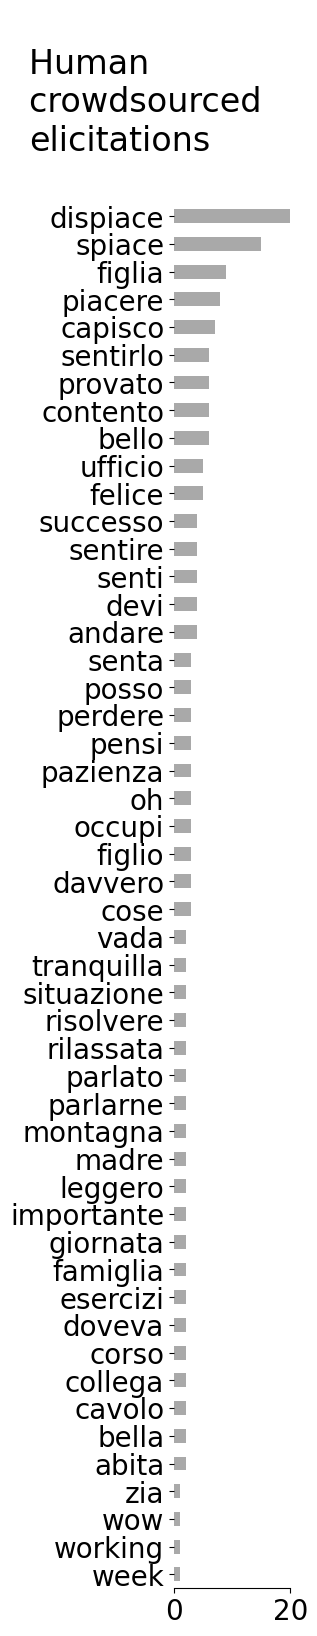
\includegraphics[height=18cm]{assets/imgs/dataset-test-set-top-50-answers-vertical.png}
        \caption{This Figure reports the top 50 most frequent tokens in the crowdsourced eliciting questions.}
        \label{sub:persona-narrative-elicitation-comparison-distribution-human}
        % 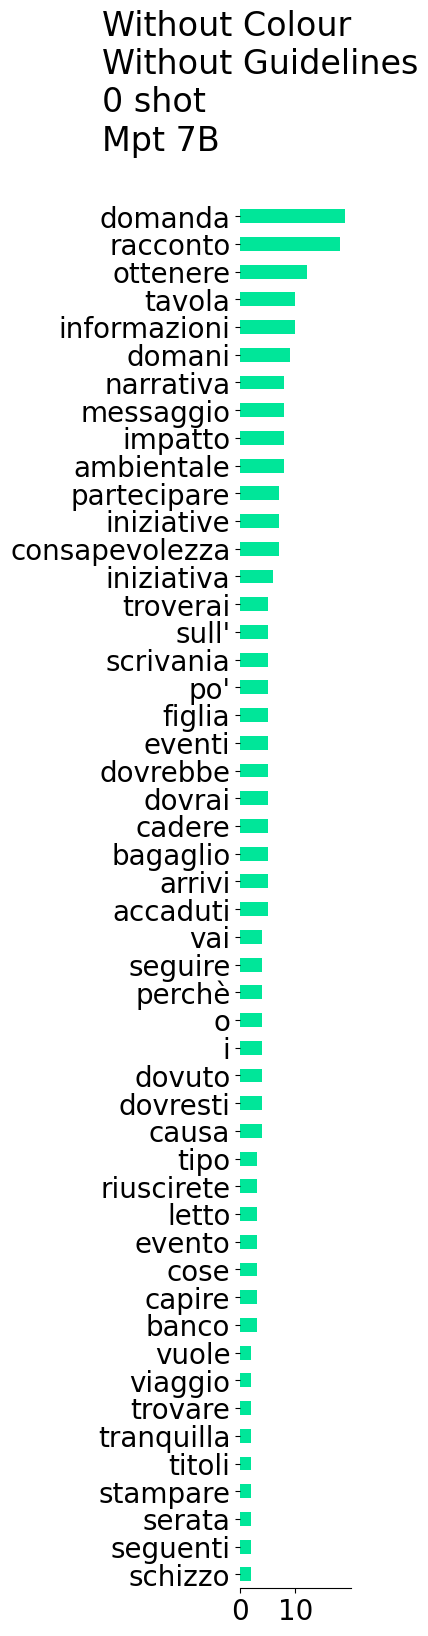
\includegraphics[height=10cm]{assets/imgs/tokens-vertical/token_distribution_no_color_no_guidelines_0_shot_mpt-7b.png}
    \end{subfigure}
    \hspace{-1.5cm}
    \captionsetup[subfigure]{oneside,margin={0cm,0cm}}
    \begin{subfigure}[t]{0.45\textwidth}
        \centering
        % \captionsetup{width=1\linewidth}%
        % 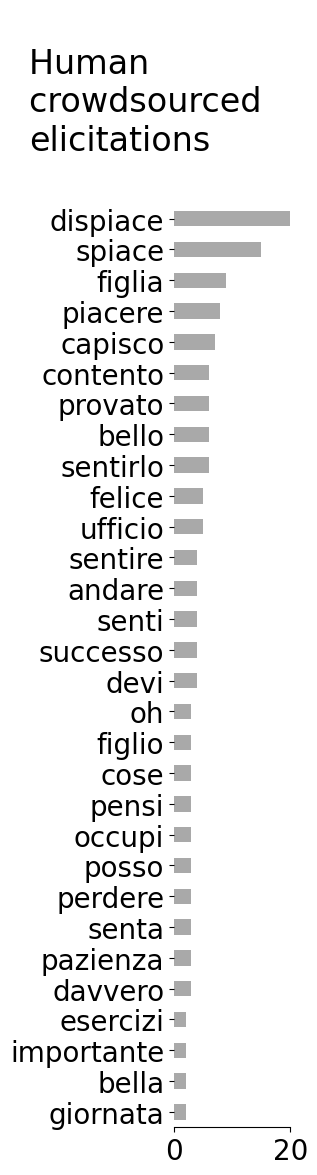
\includegraphics[width=1\textwidth]{assets/imgs/dataset-test-set-top-30-answers-vertical.png}
        \includegraphics[height=18cm]{assets/imgs/tokens-vertical/no_color/no_guidelines/0_shot/token_distribution_no_color_no_guidelines_0_shot_falcon-7b.png}
        \caption{This Figure reports the top 50 most frequent tokens from the Falcon 7B model, prompted with no colour information, without guidelines and with 0 examples.}
        \label{sub:persona-narrative-elicitation-comparison-distribution-falcon}
    \end{subfigure}
    \hspace{-2cm}
    \captionsetup[subfigure]{oneside,margin={2.5cm,0cm}}
    \begin{subfigure}[t]{0.3\textwidth}
        \centering
        % \captionsetup{justification=raggedrigh, width=1\linewidth}%
        % 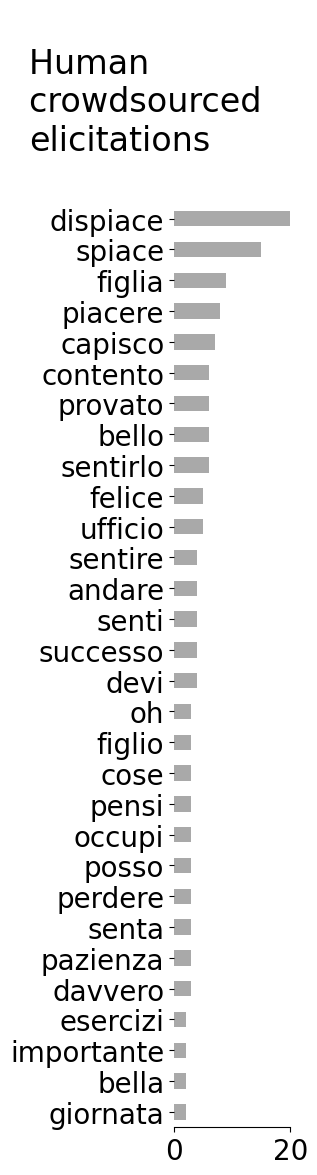
\includegraphics[width=1\textwidth]{assets/imgs/dataset-test-set-top-30-answers-vertical.png}
        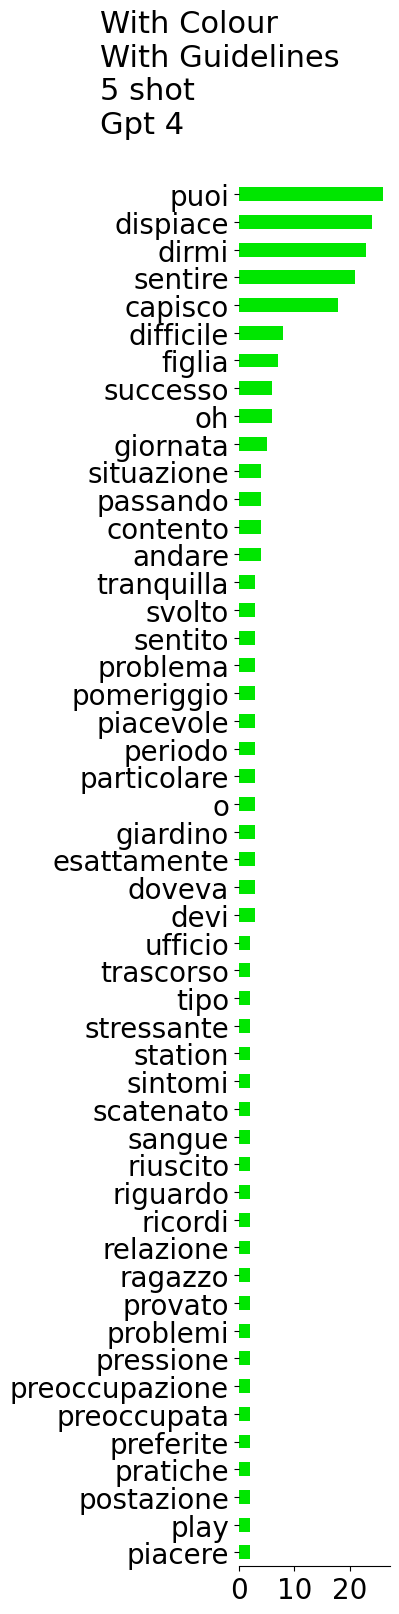
\includegraphics[height=18cm]{assets/imgs/tokens-vertical/with_color/with_guidelines/5_shot/token_distribution_with_color_with_guidelines_5_shot_gpt-4.png}
        \caption{This Figure reports the top 50 most frequent tokens from the ChatGPT 4 model, prompted with colour information, with guidelines and with 5 examples.}
            \label{sub:persona-narrative-elicitation-comparison-distribution-gpt-4}
    \end{subfigure}
    % \begin{subfigure}[b]{1\textwidth}
    %     \centering
    %     \includegraphics[width=1\textwidth]{assets/imgs/tokens/token_distribution_no_color_no_guidelines_0_shot_falcon-7b.png}
    % \end{subfigure}
    % \begin{subfigure}[b]{1\textwidth}
    %     \centering
    %     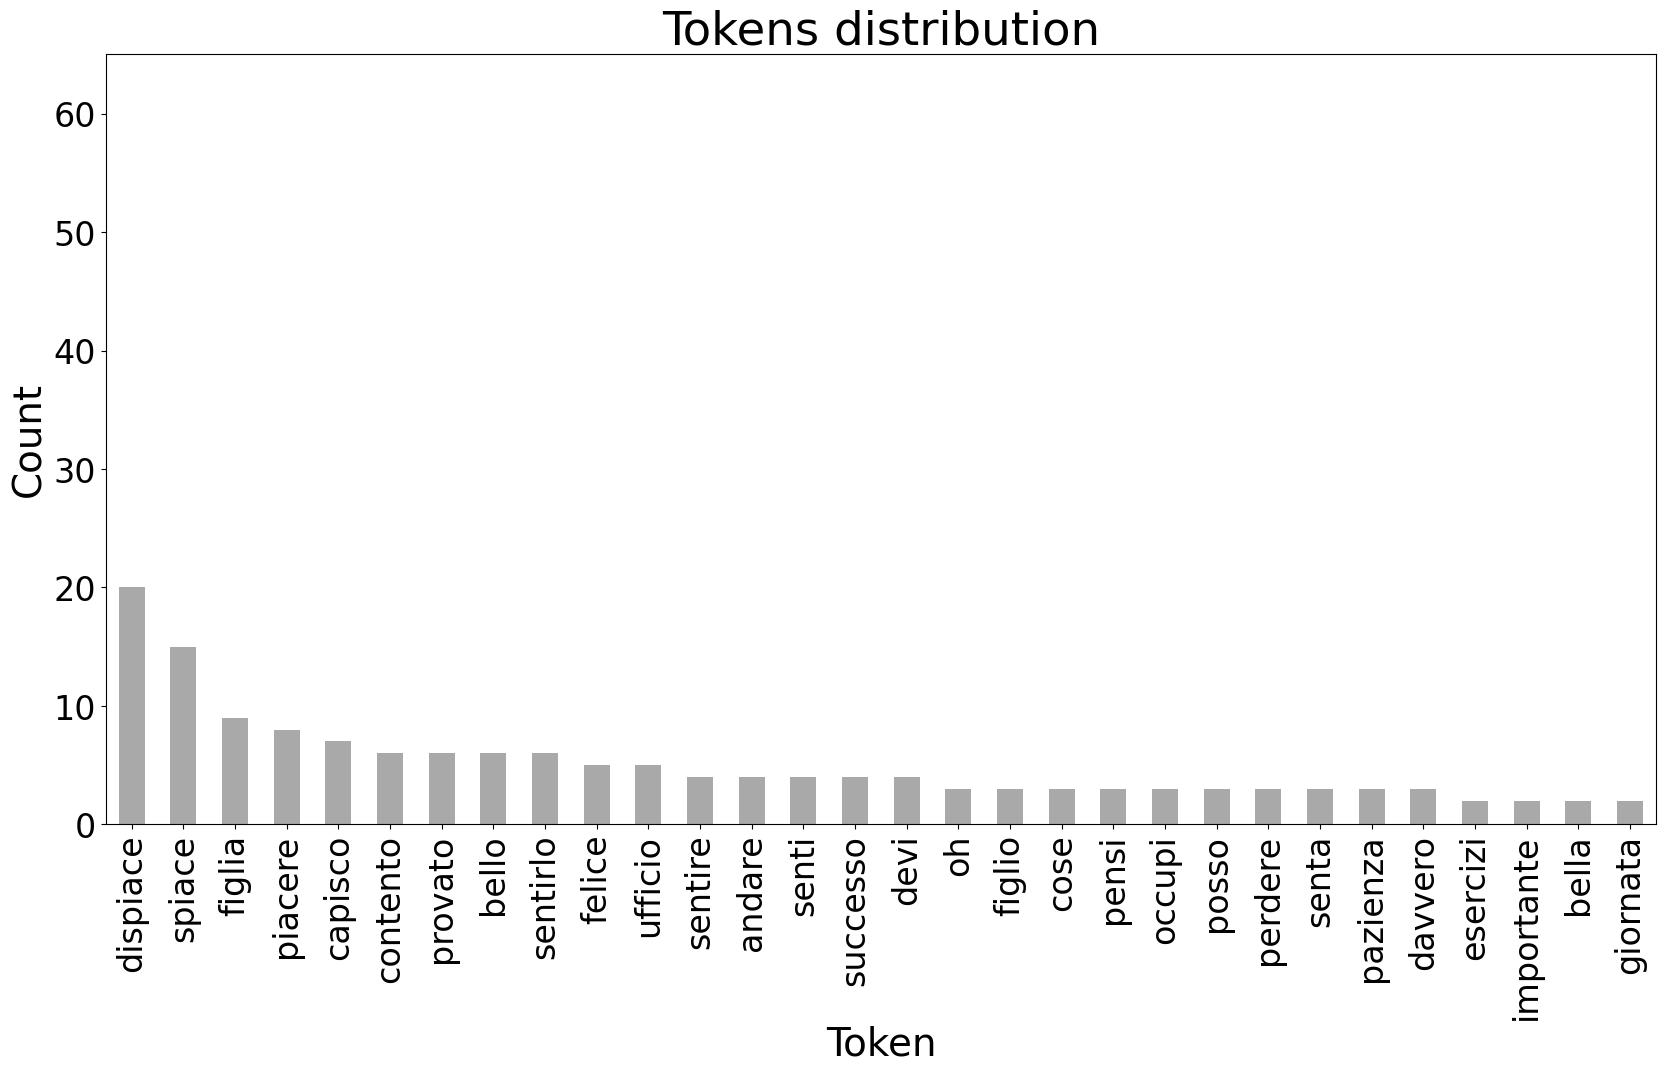
\includegraphics[width=1\textwidth]{assets/imgs/dataset-test-set-top-30-answers.png}
    % \end{subfigure}
     % \subfigure[]{\includegraphics[with=.5\linewidth]{assets/imgs/tokens/token_distribution_no_color_no_guidelines_0_shot_falcon-7b.png}}{}
    \caption{In Subfigure a), the top 50 most frequent tokens of the crowdsourced eliciting questions. In Subfigures b) and c) two examples of distributions of two different models in different experimental settings. Notice how the distribution from Gpt-4 is much closer to the human one, in particular regarding tokens like \emph{``dispiace"} and \emph{``figlia"}. %All distributions are computed using Spacy.}
    }
    \label{fig:persona-narrative-elicitation-comparison-distribution}
\end{figure}

In Figure \ref{fig:persona-narrative-elicitation-comparison-distribution} are represented the top most frequent 50 tokens of the reference crowdsourced eliciting questions and two examples of the models in different experimental settings. Considering the origin of the dataset and the experimental setup in which it was gathered, we expect many tokens such as \emph{``dispiace"} and \emph{``capisco"} because they are used to convey empathy, which was one of the requirements in the guidelines. Other relevant tokens should regard topics of discussion present in the narrative. Due to the variety of the dataset, most tokens should appear only once or few times. This is confirmed by the Subfigure \ref{sub:persona-narrative-elicitation-comparison-distribution-human}. 
In the Subfigure \ref{sub:persona-narrative-elicitation-comparison-distribution-gpt-4} it is possible to witness that ChatGPT 4 follows a similar distribution curve, with the most frequent tokens being words such as \emph{``dispiace"} and \emph{``sentire"} and then other tokens appear very rarely. 
In Subfigure \ref{sub:persona-narrative-elicitation-comparison-distribution-falcon}, we can see that this model does not follow a similar distribution at all. This confirms our findings through the Wasserstein divergence from Table \ref{tab:personal-narrative-elicitation-wasserstein}.
\begin{table}[!htbp]
    \centering
    \caption{Averages Elicitations lengths and standard deviations across the tested models. Computed using the whitespace tokenizer}
    \label{tab:personal-narrative-elicitation-token-length-std}
\setlength{\tabcolsep}{4pt}
\begin{tabular}{l|l|l|rrrr|rrrr}
\toprule
\multicolumn{3}{r}{}  & \multicolumn{4}{c|}{\rotatebox[origin=l]{0}{\thead{Average \\token length}}} & \multicolumn{4}{c}{\rotatebox[origin=l]{0}{\thead{Standard deviation \\ token length}}} \\
\midrule
\multicolumn{3}{c|}{\thead{Human}} & \multicolumn{4}{c|}{{\cellcolor[HTML]{FEE9E6}} \color[HTML]{000000}  10.42 } & \multicolumn{4}{c}{{\cellcolor[HTML]{F5FBFC}} \color[HTML]{000000} 5.12} \\
\midrule
% \multirow{1}{*}{\rotatebox[origin=l]{0}{\thead{Colour}}} & \multirow{1}{*}{\rotatebox[origin=l]{0}{\thead{Guidelines}}} & \multirow{1}{*}{\rotatebox[origin=l]{0}{\thead{Model name}}} \\
\thead{Colour} & \thead{Guidelines} & \thead{Model name} & \thead{\rotatebox[origin=l]{0}{0-shot}} & \thead{\rotatebox[origin=l]{0}{1-shot}} & \thead{\rotatebox[origin=l]{0}{3-shot}} & \thead{\rotatebox[origin=l]{0}{5-shot}} & \thead{\rotatebox[origin=l]{0}{0-shot}} & \thead{\rotatebox[origin=l]{0}{1-shot}} & \thead{\rotatebox[origin=l]{0}{3-shot}} & \thead{\rotatebox[origin=l]{0}{5-shot}}  \\
\midrule
\multirow[c]{18}{*}{\rotatebox[origin=l]{0}{\thead{Without \\ Colour}}} & \multirow[c]{9}{*}{\rotatebox[origin=l]{0}{\thead{Without \\ Guidelines}}} & Falcon 7B & {\cellcolor[HTML]{650171}} \color[HTML]{F1F1F1} 59.60 & {\cellcolor[HTML]{E7489B}} \color[HTML]{F1F1F1} 39.34 & {\cellcolor[HTML]{F871A4}} \color[HTML]{F1F1F1} 33.53 & {\cellcolor[HTML]{FBBBBD}} \color[HTML]{000000} 22.36 & {\cellcolor[HTML]{00441B}} \color[HTML]{F1F1F1} 85.52 & {\cellcolor[HTML]{63C0A0}} \color[HTML]{000000} 45.50 & {\cellcolor[HTML]{9AD8CA}} \color[HTML]{000000} 34.04 & {\cellcolor[HTML]{CAEBE5}} \color[HTML]{000000} 24.43 \\
 &  & Falcon 40B Instruct  & {\cellcolor[HTML]{FDD8D5}} \color[HTML]{000000} 15.29 & {\cellcolor[HTML]{FCCBC6}} \color[HTML]{000000} 18.84 & {\cellcolor[HTML]{FCBFBE}} \color[HTML]{000000} 21.59 & {\cellcolor[HTML]{FDD3CF}} \color[HTML]{000000} 16.67 & {\cellcolor[HTML]{EBF7FA}} \color[HTML]{000000} 10.81 & {\cellcolor[HTML]{E0F3F5}} \color[HTML]{000000} 15.95 & {\cellcolor[HTML]{E2F4F7}} \color[HTML]{000000} 15.20 & {\cellcolor[HTML]{E6F5F9}} \color[HTML]{000000} 13.31 \\
 &  & Gpt 3 & {\cellcolor[HTML]{FDDEDB}} \color[HTML]{000000} 13.66 & {\cellcolor[HTML]{FDE1DE}} \color[HTML]{000000} 12.93 & {\cellcolor[HTML]{FCCECA}} \color[HTML]{000000} 18.03 & {\cellcolor[HTML]{FCC6C2}} \color[HTML]{000000} 20.10 & {\cellcolor[HTML]{F6FCFD}} \color[HTML]{000000} 4.22 & {\cellcolor[HTML]{F5FBFD}} \color[HTML]{000000} 4.65 & {\cellcolor[HTML]{F1FAFC}} \color[HTML]{000000} 7.02 & {\cellcolor[HTML]{F2FAFC}} \color[HTML]{000000} 6.65 \\
 &  & Gpt 4 & {\cellcolor[HTML]{FCD1CD}} \color[HTML]{000000} 17.24 & {\cellcolor[HTML]{FDD4D0}} \color[HTML]{000000} 16.41 & {\cellcolor[HTML]{FCC6C1}} \color[HTML]{000000} 20.34 & {\cellcolor[HTML]{FCD0CC}} \color[HTML]{000000} 17.50 & {\cellcolor[HTML]{F6FCFD}} \color[HTML]{000000} 4.17 & {\cellcolor[HTML]{F5FBFD}} \color[HTML]{000000} 4.71 & {\cellcolor[HTML]{F6FCFD}} \color[HTML]{000000} 4.37 & {\cellcolor[HTML]{F4FBFC}} \color[HTML]{000000} 5.64 \\
 &  & Mpt 7B & {\cellcolor[HTML]{FBB0BA}} \color[HTML]{000000} 24.43 & {\cellcolor[HTML]{FCC7C3}} \color[HTML]{000000} 19.83 & {\cellcolor[HTML]{FDE1DE}} \color[HTML]{000000} 13.14 & {\cellcolor[HTML]{FBBABD}} \color[HTML]{000000} 22.43 & {\cellcolor[HTML]{8DD3C0}} \color[HTML]{000000} 36.85 & {\cellcolor[HTML]{BAE5DC}} \color[HTML]{000000} 27.72 & {\cellcolor[HTML]{EBF7FA}} \color[HTML]{000000} 10.77 & {\cellcolor[HTML]{D1EEE9}} \color[HTML]{000000} 22.27 \\
 &  & Mpt 30B Chat & {\cellcolor[HTML]{FCCECA}} \color[HTML]{000000} 17.98 & {\cellcolor[HTML]{FDE1DE}} \color[HTML]{000000} 13.12 & {\cellcolor[HTML]{FDE6E2}} \color[HTML]{000000} 11.36 & {\cellcolor[HTML]{FCD1CD}} \color[HTML]{000000} 17.09 & {\cellcolor[HTML]{B0E1D6}} \color[HTML]{000000} 29.83 & {\cellcolor[HTML]{E0F3F5}} \color[HTML]{000000} 16.04 & {\cellcolor[HTML]{E8F6FA}} \color[HTML]{000000} 12.09 & {\cellcolor[HTML]{DEF2F4}} \color[HTML]{000000} 16.80 \\
 &  & Vicuna 13B V1 & {\cellcolor[HTML]{FDDDDA}} \color[HTML]{000000} 13.91 & {\cellcolor[HTML]{FDDFDC}} \color[HTML]{000000} 13.48 & {\cellcolor[HTML]{FDE0DD}} \color[HTML]{000000} 13.21 & {\cellcolor[HTML]{FDDDDA}} \color[HTML]{000000} 13.90 & {\cellcolor[HTML]{F2FAFC}} \color[HTML]{000000} 6.27 & {\cellcolor[HTML]{ECF8FA}} \color[HTML]{000000} 10.03 & {\cellcolor[HTML]{F0F9FB}} \color[HTML]{000000} 7.73 & {\cellcolor[HTML]{E9F7FA}} \color[HTML]{000000} 11.65 \\
 &  & Vicuna 33B V1 & {\cellcolor[HTML]{FDE5E2}} \color[HTML]{000000} 11.69 & {\cellcolor[HTML]{FEE9E6}} \color[HTML]{000000} 10.28 & {\cellcolor[HTML]{FDE5E2}} \color[HTML]{000000} 11.59 & {\cellcolor[HTML]{FDE3E0}} \color[HTML]{000000} 12.43 & {\cellcolor[HTML]{F7FCFD}} \color[HTML]{000000} 3.62 & {\cellcolor[HTML]{F7FCFD}} \color[HTML]{000000} 3.91 & {\cellcolor[HTML]{F2FAFC}} \color[HTML]{000000} 6.64 & {\cellcolor[HTML]{EBF7FA}} \color[HTML]{000000} 10.76 \\
 &  & Wizard Vicuna 13B  & {\cellcolor[HTML]{FDE1DE}} \color[HTML]{000000} 12.83 & {\cellcolor[HTML]{FDE5E2}} \color[HTML]{000000} 11.62 & {\cellcolor[HTML]{FDDDDA}} \color[HTML]{000000} 14.03 & {\cellcolor[HTML]{FDDBD7}} \color[HTML]{000000} 14.72 & {\cellcolor[HTML]{F5FBFC}} \color[HTML]{000000} 4.95 & {\cellcolor[HTML]{ECF8FA}} \color[HTML]{000000} 10.33 & {\cellcolor[HTML]{EFF9FB}} \color[HTML]{000000} 8.45 & {\cellcolor[HTML]{E7F6F9}} \color[HTML]{000000} 13.08 \\

 \cmidrule{2-11}
 & \multirow[c]{9}{*}{\rotatebox[origin=lenter]{0}{\thead{With \\ Guidelines}}}& Falcon 7B & {\cellcolor[HTML]{FCCDC9}} \color[HTML]{000000} 18.19 & {\cellcolor[HTML]{FBAFBA}} \color[HTML]{000000} 24.53 & {\cellcolor[HTML]{FBBABD}} \color[HTML]{000000} 22.47 & {\cellcolor[HTML]{FBB6BC}} \color[HTML]{000000} 23.10 & {\cellcolor[HTML]{D1EEEA}} \color[HTML]{000000} 21.96 & {\cellcolor[HTML]{CDECE7}} \color[HTML]{000000} 23.69 & {\cellcolor[HTML]{CEEDE8}} \color[HTML]{000000} 23.22 & {\cellcolor[HTML]{BFE7DE}} \color[HTML]{000000} 26.68 \\
 &  & Falcon 40B Instruct  & {\cellcolor[HTML]{E84A9B}} \color[HTML]{F1F1F1} 38.97 & {\cellcolor[HTML]{FCBEBE}} \color[HTML]{000000} 21.93 & {\cellcolor[HTML]{FCC4C0}} \color[HTML]{000000} 20.71 & {\cellcolor[HTML]{FCC2BF}} \color[HTML]{000000} 20.88 & {\cellcolor[HTML]{9DDACB}} \color[HTML]{000000} 33.39 & {\cellcolor[HTML]{C5E9E2}} \color[HTML]{000000} 25.56 & {\cellcolor[HTML]{DBF2F2}} \color[HTML]{000000} 17.81 & {\cellcolor[HTML]{CEEDE8}} \color[HTML]{000000} 23.29 \\
 &  & Gpt 3 & {\cellcolor[HTML]{FCD0CC}} \color[HTML]{000000} 17.67 & {\cellcolor[HTML]{FCCCC7}} \color[HTML]{000000} 18.72 & {\cellcolor[HTML]{FCC6C2}} \color[HTML]{000000} 20.07 & {\cellcolor[HTML]{FCC6C1}} \color[HTML]{000000} 20.17 & {\cellcolor[HTML]{F1FAFC}} \color[HTML]{000000} 7.09 & {\cellcolor[HTML]{F0F9FB}} \color[HTML]{000000} 7.53 & {\cellcolor[HTML]{EEF8FB}} \color[HTML]{000000} 8.90 & {\cellcolor[HTML]{F1FAFC}} \color[HTML]{000000} 7.44 \\
 &  & Gpt 4 & {\cellcolor[HTML]{FCC6C2}} \color[HTML]{000000} 20.03 & {\cellcolor[HTML]{FCC8C3}} \color[HTML]{000000} 19.57 & {\cellcolor[HTML]{FCC0BF}} \color[HTML]{000000} 21.31 & {\cellcolor[HTML]{FCCECA}} \color[HTML]{000000} 17.98 & {\cellcolor[HTML]{F5FBFD}} \color[HTML]{000000} 4.76 & {\cellcolor[HTML]{F5FBFD}} \color[HTML]{000000} 4.71 & {\cellcolor[HTML]{F5FBFD}} \color[HTML]{000000} 4.80 & {\cellcolor[HTML]{F5FBFC}} \color[HTML]{000000} 5.11 \\
 &  & Mpt 7B & {\cellcolor[HTML]{FDD6D2}} \color[HTML]{000000} 16.02 & {\cellcolor[HTML]{FCC9C4}} \color[HTML]{000000} 19.40 & {\cellcolor[HTML]{000000}} \color[HTML]{F1F1F1} nan & {\cellcolor[HTML]{000000}} \color[HTML]{F1F1F1} nan & {\cellcolor[HTML]{E1F4F6}} \color[HTML]{000000} 15.66 & {\cellcolor[HTML]{D9F1F0}} \color[HTML]{000000} 18.86 & {\cellcolor[HTML]{000000}} \color[HTML]{F1F1F1} nan & {\cellcolor[HTML]{000000}} \color[HTML]{F1F1F1} nan \\
 &  & Mpt 30B Chat & {\cellcolor[HTML]{FDD8D5}} \color[HTML]{000000} 15.21 & {\cellcolor[HTML]{FEE7E4}} \color[HTML]{000000} 11.10 & {\cellcolor[HTML]{FDD8D5}} \color[HTML]{000000} 15.34 & {\cellcolor[HTML]{FDD9D6}} \color[HTML]{000000} 15.12 & {\cellcolor[HTML]{E1F4F6}} \color[HTML]{000000} 15.53 & {\cellcolor[HTML]{EEF8FB}} \color[HTML]{000000} 8.78 & {\cellcolor[HTML]{E8F6FA}} \color[HTML]{000000} 12.57 & {\cellcolor[HTML]{E8F6FA}} \color[HTML]{000000} 12.47 \\
 &  & Vicuna 13B V1 & {\cellcolor[HTML]{FDD5D1}} \color[HTML]{000000} 16.19 & {\cellcolor[HTML]{FCCDC9}} \color[HTML]{000000} 18.26 & {\cellcolor[HTML]{FDD7D4}} \color[HTML]{000000} 15.50 & {\cellcolor[HTML]{FDE0DD}} \color[HTML]{000000} 13.16 & {\cellcolor[HTML]{E1F4F6}} \color[HTML]{000000} 15.51 & {\cellcolor[HTML]{D8F0EF}} \color[HTML]{000000} 19.03 & {\cellcolor[HTML]{E7F6F9}} \color[HTML]{000000} 12.96 & {\cellcolor[HTML]{E6F5F9}} \color[HTML]{000000} 13.38 \\
 &  & Vicuna 33B V1 & {\cellcolor[HTML]{FDE1DE}} \color[HTML]{000000} 12.81 & {\cellcolor[HTML]{FCCBC6}} \color[HTML]{000000} 18.81 & {\cellcolor[HTML]{FDDEDB}} \color[HTML]{000000} 13.83 & {\cellcolor[HTML]{FDD9D6}} \color[HTML]{000000} 15.12 & {\cellcolor[HTML]{E1F4F6}} \color[HTML]{000000} 15.64 & {\cellcolor[HTML]{DFF3F4}} \color[HTML]{000000} 16.66 & {\cellcolor[HTML]{EBF7FA}} \color[HTML]{000000} 10.82 & {\cellcolor[HTML]{E8F6FA}} \color[HTML]{000000} 12.27 \\
 &  & Wizard Vicuna 13B  & {\cellcolor[HTML]{FFF3F0}} \color[HTML]{000000} 7.26 & {\cellcolor[HTML]{FEE7E4}} \color[HTML]{000000} 10.95 & {\cellcolor[HTML]{FCD1CD}} \color[HTML]{000000} 17.00 & {\cellcolor[HTML]{FDE4E0}} \color[HTML]{000000} 12.07 & {\cellcolor[HTML]{EDF8FB}} \color[HTML]{000000} 9.33 & {\cellcolor[HTML]{E9F7FA}} \color[HTML]{000000} 11.77 & {\cellcolor[HTML]{E3F4F8}} \color[HTML]{000000} 14.68 & {\cellcolor[HTML]{EDF8FB}} \color[HTML]{000000} 9.31 \\

\midrule
\multirow[c]{18}{*}{\rotatebox[origin=l]{0}{\thead{With\\ Colour}}} & \multirow[c]{9}{*}{\rotatebox[origin=l]{0}{\thead{Without \\ Guidelines}}} & Falcon 7B & {\cellcolor[HTML]{49006A}} \color[HTML]{F1F1F1} 63.81 & {\cellcolor[HTML]{DC3397}} \color[HTML]{F1F1F1} 42.24 & {\cellcolor[HTML]{FBB8BC}} \color[HTML]{000000} 23.09 & {\cellcolor[HTML]{F98BAE}} \color[HTML]{000000} 30.31 & {\cellcolor[HTML]{006729}} \color[HTML]{F1F1F1} 76.58 & {\cellcolor[HTML]{6AC4A7}} \color[HTML]{000000} 43.73 & {\cellcolor[HTML]{C2E8E0}} \color[HTML]{000000} 26.12 & {\cellcolor[HTML]{B5E3D9}} \color[HTML]{000000} 28.61 \\
 &  & Falcon 40B Instruct  & {\cellcolor[HTML]{FCCECA}} \color[HTML]{000000} 17.93 & {\cellcolor[HTML]{FDD7D3}} \color[HTML]{000000} 15.81 & {\cellcolor[HTML]{FDD5D1}} \color[HTML]{000000} 16.22 & {\cellcolor[HTML]{FCCCC7}} \color[HTML]{000000} 18.72 & {\cellcolor[HTML]{DFF3F4}} \color[HTML]{000000} 16.56 & {\cellcolor[HTML]{E8F6FA}} \color[HTML]{000000} 12.21 & {\cellcolor[HTML]{EAF7FA}} \color[HTML]{000000} 11.22 & {\cellcolor[HTML]{DEF2F4}} \color[HTML]{000000} 16.97 \\
 &  & Gpt 3 & {\cellcolor[HTML]{FDDCD8}} \color[HTML]{000000} 14.34 & {\cellcolor[HTML]{FDE4E0}} \color[HTML]{000000} 12.24 & {\cellcolor[HTML]{FCC1BF}} \color[HTML]{000000} 21.28 & {\cellcolor[HTML]{FCC4C0}} \color[HTML]{000000} 20.69 & {\cellcolor[HTML]{F5FBFD}} \color[HTML]{000000} 4.60 & {\cellcolor[HTML]{F5FBFC}} \color[HTML]{000000} 5.10 & {\cellcolor[HTML]{F2FAFC}} \color[HTML]{000000} 6.51 & {\cellcolor[HTML]{F4FBFC}} \color[HTML]{000000} 5.65 \\
 &  & Gpt 4 & {\cellcolor[HTML]{FCD1CD}} \color[HTML]{000000} 17.17 & {\cellcolor[HTML]{FCD2CE}} \color[HTML]{000000} 16.78 & {\cellcolor[HTML]{FCC4C0}} \color[HTML]{000000} 20.71 & {\cellcolor[HTML]{FCD0CC}} \color[HTML]{000000} 17.62 & {\cellcolor[HTML]{F5FBFC}} \color[HTML]{000000} 4.96 & {\cellcolor[HTML]{F4FBFC}} \color[HTML]{000000} 5.47 & {\cellcolor[HTML]{F4FBFC}} \color[HTML]{000000} 5.34 & {\cellcolor[HTML]{F4FBFC}} \color[HTML]{000000} 5.52 \\
 &  & Mpt 7B & {\cellcolor[HTML]{FBADB9}} \color[HTML]{000000} 24.97 & {\cellcolor[HTML]{EA4D9C}} \color[HTML]{F1F1F1} 38.67 & {\cellcolor[HTML]{FDE3E0}} \color[HTML]{000000} 12.33 & {\cellcolor[HTML]{FCD2CE}} \color[HTML]{000000} 16.83 & {\cellcolor[HTML]{6FC6AA}} \color[HTML]{000000} 42.69 & {\cellcolor[HTML]{9CD9CA}} \color[HTML]{000000} 33.74 & {\cellcolor[HTML]{E8F6FA}} \color[HTML]{000000} 12.51 & {\cellcolor[HTML]{D8F0EF}} \color[HTML]{000000} 19.27 \\
 &  & Mpt 30B Chat & {\cellcolor[HTML]{FDD9D6}} \color[HTML]{000000} 15.16 & {\cellcolor[HTML]{FCCFCB}} \color[HTML]{000000} 17.78 & {\cellcolor[HTML]{FEE9E6}} \color[HTML]{000000} 10.41 & {\cellcolor[HTML]{FBB9BC}} \color[HTML]{000000} 22.81 & {\cellcolor[HTML]{D3EEEB}} \color[HTML]{000000} 21.39 & {\cellcolor[HTML]{DDF2F3}} \color[HTML]{000000} 17.07 & {\cellcolor[HTML]{ECF8FB}} \color[HTML]{000000} 9.88 & {\cellcolor[HTML]{DBF1F1}} \color[HTML]{000000} 18.23 \\
 &  & Vicuna 13B V1 & {\cellcolor[HTML]{FDE0DD}} \color[HTML]{000000} 13.33 & {\cellcolor[HTML]{FDD7D3}} \color[HTML]{000000} 15.83 & {\cellcolor[HTML]{FEE9E6}} \color[HTML]{000000} 10.40 & {\cellcolor[HTML]{FDD7D3}} \color[HTML]{000000} 15.78 & {\cellcolor[HTML]{F4FBFC}} \color[HTML]{000000} 5.43 & {\cellcolor[HTML]{E3F4F8}} \color[HTML]{000000} 14.56 & {\cellcolor[HTML]{F0F9FB}} \color[HTML]{000000} 7.99 & {\cellcolor[HTML]{E5F5F9}} \color[HTML]{000000} 13.90 \\
 &  & Vicuna 33B V1 & {\cellcolor[HTML]{FDDFDC}} \color[HTML]{000000} 13.59 & {\cellcolor[HTML]{FDD7D3}} \color[HTML]{000000} 15.69 & {\cellcolor[HTML]{FEEAE7}} \color[HTML]{000000} 10.03 & {\cellcolor[HTML]{FDDFDC}} \color[HTML]{000000} 13.40 & {\cellcolor[HTML]{EDF8FB}} \color[HTML]{000000} 9.06 & {\cellcolor[HTML]{E2F4F7}} \color[HTML]{000000} 15.28 & {\cellcolor[HTML]{E9F7FA}} \color[HTML]{000000} 11.88 & {\cellcolor[HTML]{E6F5F9}} \color[HTML]{000000} 13.24 \\
 &  & Wizard Vicuna 13B  & {\cellcolor[HTML]{FDDFDC}} \color[HTML]{000000} 13.47 & {\cellcolor[HTML]{FEE9E6}} \color[HTML]{000000} 10.31 & {\cellcolor[HTML]{FEE7E4}} \color[HTML]{000000} 10.91 & {\cellcolor[HTML]{FDDDDA}} \color[HTML]{000000} 13.97 & {\cellcolor[HTML]{F4FBFC}} \color[HTML]{000000} 5.47 & {\cellcolor[HTML]{F4FBFC}} \color[HTML]{000000} 5.60 & {\cellcolor[HTML]{EDF8FB}} \color[HTML]{000000} 9.67 & {\cellcolor[HTML]{EFF9FB}} \color[HTML]{000000} 8.73 \\

  \cmidrule{2-11}
 & \multirow[c]{9}{*}{\rotatebox[origin=l]{0}{\thead{With \\ Guidelines}}} & Falcon 7B & {\cellcolor[HTML]{FCD1CD}} \color[HTML]{000000} 17.26 & {\cellcolor[HTML]{FCBCBD}} \color[HTML]{000000} 22.14 & {\cellcolor[HTML]{FCD2CE}} \color[HTML]{000000} 16.78 & {\cellcolor[HTML]{FCD0CC}} \color[HTML]{000000} 17.50 & {\cellcolor[HTML]{D8F0EF}} \color[HTML]{000000} 19.28 & {\cellcolor[HTML]{CDECE6}} \color[HTML]{000000} 23.88 & {\cellcolor[HTML]{D8F0EF}} \color[HTML]{000000} 19.11 & {\cellcolor[HTML]{D1EEE9}} \color[HTML]{000000} 22.21 \\
 &  & Falcon 40B Instruct  & {\cellcolor[HTML]{EA4F9C}} \color[HTML]{F1F1F1} 38.47 & {\cellcolor[HTML]{FA9EB5}} \color[HTML]{000000} 27.67 & {\cellcolor[HTML]{F25D9F}} \color[HTML]{F1F1F1} 36.38 & {\cellcolor[HTML]{E94B9C}} \color[HTML]{F1F1F1} 38.79 & {\cellcolor[HTML]{94D6C5}} \color[HTML]{000000} 35.43 & {\cellcolor[HTML]{A4DCCF}} \color[HTML]{000000} 32.40 & {\cellcolor[HTML]{97D7C7}} \color[HTML]{000000} 34.87 & {\cellcolor[HTML]{A8DED2}} \color[HTML]{000000} 31.30 \\
 &  & Gpt 3 & {\cellcolor[HTML]{FCCAC5}} \color[HTML]{000000} 19.22 & {\cellcolor[HTML]{FCC6C2}} \color[HTML]{000000} 20.02 & {\cellcolor[HTML]{FCC6C1}} \color[HTML]{000000} 20.22 & {\cellcolor[HTML]{FCC4C0}} \color[HTML]{000000} 20.67 & {\cellcolor[HTML]{EBF7FA}} \color[HTML]{000000} 10.52 & {\cellcolor[HTML]{EBF7FA}} \color[HTML]{000000} 10.38 & {\cellcolor[HTML]{F1FAFC}} \color[HTML]{000000} 6.93 & {\cellcolor[HTML]{F1FAFC}} \color[HTML]{000000} 6.93 \\
 &  & Gpt 4 & {\cellcolor[HTML]{FCC6C2}} \color[HTML]{000000} 20.05 & {\cellcolor[HTML]{FCCAC5}} \color[HTML]{000000} 19.03 & {\cellcolor[HTML]{FCBEBE}} \color[HTML]{000000} 21.84 & {\cellcolor[HTML]{FCCAC5}} \color[HTML]{000000} 19.09 & {\cellcolor[HTML]{F5FBFD}} \color[HTML]{000000} 4.64 & {\cellcolor[HTML]{F6FCFD}} \color[HTML]{000000} 4.49 & {\cellcolor[HTML]{F6FCFD}} \color[HTML]{000000} 4.32 & {\cellcolor[HTML]{F5FBFD}} \color[HTML]{000000} 4.65 \\
 &  & Mpt 7B & {\cellcolor[HTML]{FDD6D2}} \color[HTML]{000000} 15.91 & {\cellcolor[HTML]{FCD1CD}} \color[HTML]{000000} 17.19 & {\cellcolor[HTML]{000000}} \color[HTML]{F1F1F1} nan & {\cellcolor[HTML]{000000}} \color[HTML]{F1F1F1} nan & {\cellcolor[HTML]{DDF2F3}} \color[HTML]{000000} 17.35 & {\cellcolor[HTML]{D8F0EF}} \color[HTML]{000000} 19.21 & {\cellcolor[HTML]{000000}} \color[HTML]{F1F1F1} nan & {\cellcolor[HTML]{000000}} \color[HTML]{F1F1F1} nan \\
 &  & Mpt 30B Chat & {\cellcolor[HTML]{FCC1BF}} \color[HTML]{000000} 21.17 & {\cellcolor[HTML]{FBBABD}} \color[HTML]{000000} 22.59 & {\cellcolor[HTML]{000000}} \color[HTML]{F1F1F1} nan & {\cellcolor[HTML]{000000}} \color[HTML]{F1F1F1} nan & {\cellcolor[HTML]{D5EFED}} \color[HTML]{000000} 20.56 & {\cellcolor[HTML]{D4EFEC}} \color[HTML]{000000} 21.14 & {\cellcolor[HTML]{000000}} \color[HTML]{F1F1F1} nan & {\cellcolor[HTML]{000000}} \color[HTML]{F1F1F1} nan \\
 &  & Vicuna 13B V1 & {\cellcolor[HTML]{FCD2CE}} \color[HTML]{000000} 16.95 & {\cellcolor[HTML]{FDDDDA}} \color[HTML]{000000} 14.03 & {\cellcolor[HTML]{FDE0DD}} \color[HTML]{000000} 13.28 & {\cellcolor[HTML]{FEECE9}} \color[HTML]{000000} 9.31 & {\cellcolor[HTML]{DEF2F4}} \color[HTML]{000000} 17.02 & {\cellcolor[HTML]{E2F4F7}} \color[HTML]{000000} 15.41 & {\cellcolor[HTML]{E2F4F7}} \color[HTML]{000000} 15.35 & {\cellcolor[HTML]{F2FAFC}} \color[HTML]{000000} 6.27 \\
 &  & Vicuna 33B V1 & {\cellcolor[HTML]{FDD6D2}} \color[HTML]{000000} 16.05 & {\cellcolor[HTML]{FDE6E2}} \color[HTML]{000000} 11.38 & {\cellcolor[HTML]{FFF2EE}} \color[HTML]{000000} 7.66 & {\cellcolor[HTML]{FFF7F3}} \color[HTML]{000000} 5.91 & {\cellcolor[HTML]{D9F1F0}} \color[HTML]{000000} 18.74 & {\cellcolor[HTML]{E3F4F7}} \color[HTML]{000000} 15.11 & {\cellcolor[HTML]{E8F6FA}} \color[HTML]{000000} 12.12 & {\cellcolor[HTML]{EBF7FA}} \color[HTML]{000000} 10.64 \\
 &  & Wizard Vicuna 13B  & {\cellcolor[HTML]{FEEEEB}} \color[HTML]{000000} 8.72 & {\cellcolor[HTML]{FEF1ED}} \color[HTML]{000000} 7.88 & {\cellcolor[HTML]{FDE3E0}} \color[HTML]{000000} 12.45 & {\cellcolor[HTML]{FEECE9}} \color[HTML]{000000} 9.48 & {\cellcolor[HTML]{EBF7FA}} \color[HTML]{000000} 10.63 & {\cellcolor[HTML]{E7F6F9}} \color[HTML]{000000} 12.68 & {\cellcolor[HTML]{EAF7FA}} \color[HTML]{000000} 11.14 & {\cellcolor[HTML]{E9F7FA}} \color[HTML]{000000} 11.89 \\

\bottomrule

\end{tabular}
\setlength{\tabcolsep}{6pt}
\end{table}

% \begin{table}[ht]
    \centering
    \caption{Standard deviation on Elicitations lengths across the tested models. Computed using the whitespace tokenizer.}
    \label{tab:personal-narrative-elicitation-token-std}
    \begin{tabular}{l|l|l|rrrr}
    \toprule
\multicolumn{3}{r}{\thead{Standard Deviation Reference Human \\ Elicitation Token Length}} & \multicolumn{4}{r}{{\cellcolor[HTML]{F5FBFC}} \color[HTML]{000000} 5.12} \\
    \midrule
    \thead{Colour} & \thead{Guidelines} & \thead{Model name} & \thead{0-shot} & \thead{1-shot} & \thead{3-shot} & \thead{5-shot} \\
    \midrule
    \multirow[c]{18}{*}{\thead{Without\\ Colour}} & \multirow[c]{9}{*}{\thead{Without\\ Guidelines}}  & Falcon 7B & {\cellcolor[HTML]{00441B}} \color[HTML]{F1F1F1} 85.52 & {\cellcolor[HTML]{63C0A0}} \color[HTML]{000000} 45.50 & {\cellcolor[HTML]{9AD8CA}} \color[HTML]{000000} 34.04 & {\cellcolor[HTML]{CAEBE5}} \color[HTML]{000000} 24.43 \\
 &  & Falcon 40B Instruct & {\cellcolor[HTML]{EBF7FA}} \color[HTML]{000000} 10.81 & {\cellcolor[HTML]{E0F3F5}} \color[HTML]{000000} 15.95 & {\cellcolor[HTML]{E2F4F7}} \color[HTML]{000000} 15.20 & {\cellcolor[HTML]{E6F5F9}} \color[HTML]{000000} 13.31 \\
 &  & Gpt 3 & {\cellcolor[HTML]{F6FCFD}} \color[HTML]{000000} 4.22 & {\cellcolor[HTML]{F5FBFD}} \color[HTML]{000000} 4.65 & {\cellcolor[HTML]{F1FAFC}} \color[HTML]{000000} 7.02 & {\cellcolor[HTML]{F2FAFC}} \color[HTML]{000000} 6.65 \\
 &  & Gpt 4 & {\cellcolor[HTML]{F6FCFD}} \color[HTML]{000000} 4.17 & {\cellcolor[HTML]{F5FBFD}} \color[HTML]{000000} 4.71 & {\cellcolor[HTML]{F6FCFD}} \color[HTML]{000000} 4.37 & {\cellcolor[HTML]{F4FBFC}} \color[HTML]{000000} 5.64 \\
 &  & Mpt 7B & {\cellcolor[HTML]{8DD3C0}} \color[HTML]{000000} 36.85 & {\cellcolor[HTML]{BAE5DC}} \color[HTML]{000000} 27.72 & {\cellcolor[HTML]{EBF7FA}} \color[HTML]{000000} 10.77 & {\cellcolor[HTML]{D1EEE9}} \color[HTML]{000000} 22.27 \\
 &  & Mpt 30B Chat & {\cellcolor[HTML]{B0E1D6}} \color[HTML]{000000} 29.83 & {\cellcolor[HTML]{E0F3F5}} \color[HTML]{000000} 16.04 & {\cellcolor[HTML]{E8F6FA}} \color[HTML]{000000} 12.09 & {\cellcolor[HTML]{DEF2F4}} \color[HTML]{000000} 16.80 \\
 &  & Vicuna 13B V1 & {\cellcolor[HTML]{F2FAFC}} \color[HTML]{000000} 6.27 & {\cellcolor[HTML]{ECF8FA}} \color[HTML]{000000} 10.03 & {\cellcolor[HTML]{F0F9FB}} \color[HTML]{000000} 7.73 & {\cellcolor[HTML]{E9F7FA}} \color[HTML]{000000} 11.65 \\
 &  & Vicuna 33B V1 & {\cellcolor[HTML]{F7FCFD}} \color[HTML]{000000} 3.62 & {\cellcolor[HTML]{F7FCFD}} \color[HTML]{000000} 3.91 & {\cellcolor[HTML]{F2FAFC}} \color[HTML]{000000} 6.64 & {\cellcolor[HTML]{EBF7FA}} \color[HTML]{000000} 10.76 \\
 &  & Wizard Vicuna 13B Uncensored HF & {\cellcolor[HTML]{F5FBFC}} \color[HTML]{000000} 4.95 & {\cellcolor[HTML]{ECF8FA}} \color[HTML]{000000} 10.33 & {\cellcolor[HTML]{EFF9FB}} \color[HTML]{000000} 8.45 & {\cellcolor[HTML]{E7F6F9}} \color[HTML]{000000} 13.08 \\

     \cmidrule{2-7}
     & \multirow[c]{9}{*}{\thead{With\\ Guidelines}} & Falcon 7B & {\cellcolor[HTML]{D1EEEA}} \color[HTML]{000000} 21.96 & {\cellcolor[HTML]{CDECE7}} \color[HTML]{000000} 23.69 & {\cellcolor[HTML]{CEEDE8}} \color[HTML]{000000} 23.22 & {\cellcolor[HTML]{BFE7DE}} \color[HTML]{000000} 26.68 \\
 &  & Falcon 40B Instruct & {\cellcolor[HTML]{9DDACB}} \color[HTML]{000000} 33.39 & {\cellcolor[HTML]{C5E9E2}} \color[HTML]{000000} 25.56 & {\cellcolor[HTML]{DBF2F2}} \color[HTML]{000000} 17.81 & {\cellcolor[HTML]{CEEDE8}} \color[HTML]{000000} 23.29 \\
 &  & Gpt 3 & {\cellcolor[HTML]{F1FAFC}} \color[HTML]{000000} 7.09 & {\cellcolor[HTML]{F0F9FB}} \color[HTML]{000000} 7.53 & {\cellcolor[HTML]{EEF8FB}} \color[HTML]{000000} 8.90 & {\cellcolor[HTML]{F1FAFC}} \color[HTML]{000000} 7.44 \\
 &  & Gpt 4 & {\cellcolor[HTML]{F5FBFD}} \color[HTML]{000000} 4.76 & {\cellcolor[HTML]{F5FBFD}} \color[HTML]{000000} 4.71 & {\cellcolor[HTML]{F5FBFD}} \color[HTML]{000000} 4.80 & {\cellcolor[HTML]{F5FBFC}} \color[HTML]{000000} 5.11 \\
 &  & Mpt 7B & {\cellcolor[HTML]{E1F4F6}} \color[HTML]{000000} 15.66 & {\cellcolor[HTML]{D9F1F0}} \color[HTML]{000000} 18.86 & {\cellcolor[HTML]{000000}} \color[HTML]{F1F1F1} nan & {\cellcolor[HTML]{000000}} \color[HTML]{F1F1F1} nan \\
 &  & Mpt 30B Chat & {\cellcolor[HTML]{E1F4F6}} \color[HTML]{000000} 15.53 & {\cellcolor[HTML]{EEF8FB}} \color[HTML]{000000} 8.78 & {\cellcolor[HTML]{E8F6FA}} \color[HTML]{000000} 12.57 & {\cellcolor[HTML]{E8F6FA}} \color[HTML]{000000} 12.47 \\
 &  & Vicuna 13B V1 & {\cellcolor[HTML]{E1F4F6}} \color[HTML]{000000} 15.51 & {\cellcolor[HTML]{D8F0EF}} \color[HTML]{000000} 19.03 & {\cellcolor[HTML]{E7F6F9}} \color[HTML]{000000} 12.96 & {\cellcolor[HTML]{E6F5F9}} \color[HTML]{000000} 13.38 \\
 &  & Vicuna 33B V1 & {\cellcolor[HTML]{E1F4F6}} \color[HTML]{000000} 15.64 & {\cellcolor[HTML]{DFF3F4}} \color[HTML]{000000} 16.66 & {\cellcolor[HTML]{EBF7FA}} \color[HTML]{000000} 10.82 & {\cellcolor[HTML]{E8F6FA}} \color[HTML]{000000} 12.27 \\
 &  & Wizard Vicuna 13B Uncensored HF & {\cellcolor[HTML]{EDF8FB}} \color[HTML]{000000} 9.33 & {\cellcolor[HTML]{E9F7FA}} \color[HTML]{000000} 11.77 & {\cellcolor[HTML]{E3F4F8}} \color[HTML]{000000} 14.68 & {\cellcolor[HTML]{EDF8FB}} \color[HTML]{000000} 9.31 \\

     \midrule
    \multirow[c]{18}{*}{\thead{With\\ Colour}} & \multirow[c]{9}{*}{\thead{Without\\ Guidelines}} & Falcon 7B & {\cellcolor[HTML]{006729}} \color[HTML]{F1F1F1} 76.58 & {\cellcolor[HTML]{6AC4A7}} \color[HTML]{000000} 43.73 & {\cellcolor[HTML]{C2E8E0}} \color[HTML]{000000} 26.12 & {\cellcolor[HTML]{B5E3D9}} \color[HTML]{000000} 28.61 \\
 &  & Falcon 40B Instruct & {\cellcolor[HTML]{DFF3F4}} \color[HTML]{000000} 16.56 & {\cellcolor[HTML]{E8F6FA}} \color[HTML]{000000} 12.21 & {\cellcolor[HTML]{EAF7FA}} \color[HTML]{000000} 11.22 & {\cellcolor[HTML]{DEF2F4}} \color[HTML]{000000} 16.97 \\
 &  & Gpt 3 & {\cellcolor[HTML]{F5FBFD}} \color[HTML]{000000} 4.60 & {\cellcolor[HTML]{F5FBFC}} \color[HTML]{000000} 5.10 & {\cellcolor[HTML]{F2FAFC}} \color[HTML]{000000} 6.51 & {\cellcolor[HTML]{F4FBFC}} \color[HTML]{000000} 5.65 \\
 &  & Gpt 4 & {\cellcolor[HTML]{F5FBFC}} \color[HTML]{000000} 4.96 & {\cellcolor[HTML]{F4FBFC}} \color[HTML]{000000} 5.47 & {\cellcolor[HTML]{F4FBFC}} \color[HTML]{000000} 5.34 & {\cellcolor[HTML]{F4FBFC}} \color[HTML]{000000} 5.52 \\
 &  & Mpt 7B & {\cellcolor[HTML]{6FC6AA}} \color[HTML]{000000} 42.69 & {\cellcolor[HTML]{9CD9CA}} \color[HTML]{000000} 33.74 & {\cellcolor[HTML]{E8F6FA}} \color[HTML]{000000} 12.51 & {\cellcolor[HTML]{D8F0EF}} \color[HTML]{000000} 19.27 \\
 &  & Mpt 30B Chat & {\cellcolor[HTML]{D3EEEB}} \color[HTML]{000000} 21.39 & {\cellcolor[HTML]{DDF2F3}} \color[HTML]{000000} 17.07 & {\cellcolor[HTML]{ECF8FB}} \color[HTML]{000000} 9.88 & {\cellcolor[HTML]{DBF1F1}} \color[HTML]{000000} 18.23 \\
 &  & Vicuna 13B V1 & {\cellcolor[HTML]{F4FBFC}} \color[HTML]{000000} 5.43 & {\cellcolor[HTML]{E3F4F8}} \color[HTML]{000000} 14.56 & {\cellcolor[HTML]{F0F9FB}} \color[HTML]{000000} 7.99 & {\cellcolor[HTML]{E5F5F9}} \color[HTML]{000000} 13.90 \\
 &  & Vicuna 33B V1 & {\cellcolor[HTML]{EDF8FB}} \color[HTML]{000000} 9.06 & {\cellcolor[HTML]{E2F4F7}} \color[HTML]{000000} 15.28 & {\cellcolor[HTML]{E9F7FA}} \color[HTML]{000000} 11.88 & {\cellcolor[HTML]{E6F5F9}} \color[HTML]{000000} 13.24 \\
 &  & Wizard Vicuna 13B Uncensored HF & {\cellcolor[HTML]{F4FBFC}} \color[HTML]{000000} 5.47 & {\cellcolor[HTML]{F4FBFC}} \color[HTML]{000000} 5.60 & {\cellcolor[HTML]{EDF8FB}} \color[HTML]{000000} 9.67 & {\cellcolor[HTML]{EFF9FB}} \color[HTML]{000000} 8.73 \\

     \cmidrule{2-7}
     & \multirow[c]{9}{*}{\thead{With\\ Guidelines}}& Falcon 7B & {\cellcolor[HTML]{D8F0EF}} \color[HTML]{000000} 19.28 & {\cellcolor[HTML]{CDECE6}} \color[HTML]{000000} 23.88 & {\cellcolor[HTML]{D8F0EF}} \color[HTML]{000000} 19.11 & {\cellcolor[HTML]{D1EEE9}} \color[HTML]{000000} 22.21 \\
 &  & Falcon 40B Instruct & {\cellcolor[HTML]{94D6C5}} \color[HTML]{000000} 35.43 & {\cellcolor[HTML]{A4DCCF}} \color[HTML]{000000} 32.40 & {\cellcolor[HTML]{97D7C7}} \color[HTML]{000000} 34.87 & {\cellcolor[HTML]{A8DED2}} \color[HTML]{000000} 31.30 \\
 &  & Gpt 3 & {\cellcolor[HTML]{EBF7FA}} \color[HTML]{000000} 10.52 & {\cellcolor[HTML]{EBF7FA}} \color[HTML]{000000} 10.38 & {\cellcolor[HTML]{F1FAFC}} \color[HTML]{000000} 6.93 & {\cellcolor[HTML]{F1FAFC}} \color[HTML]{000000} 6.93 \\
 &  & Gpt 4 & {\cellcolor[HTML]{F5FBFD}} \color[HTML]{000000} 4.64 & {\cellcolor[HTML]{F6FCFD}} \color[HTML]{000000} 4.49 & {\cellcolor[HTML]{F6FCFD}} \color[HTML]{000000} 4.32 & {\cellcolor[HTML]{F5FBFD}} \color[HTML]{000000} 4.65 \\
 &  & Mpt 7B & {\cellcolor[HTML]{DDF2F3}} \color[HTML]{000000} 17.35 & {\cellcolor[HTML]{D8F0EF}} \color[HTML]{000000} 19.21 & {\cellcolor[HTML]{000000}} \color[HTML]{F1F1F1} nan & {\cellcolor[HTML]{000000}} \color[HTML]{F1F1F1} nan \\
 &  & Mpt 30B Chat & {\cellcolor[HTML]{D5EFED}} \color[HTML]{000000} 20.56 & {\cellcolor[HTML]{D4EFEC}} \color[HTML]{000000} 21.14 & {\cellcolor[HTML]{000000}} \color[HTML]{F1F1F1} nan & {\cellcolor[HTML]{000000}} \color[HTML]{F1F1F1} nan \\
 &  & Vicuna 13B V1 & {\cellcolor[HTML]{DEF2F4}} \color[HTML]{000000} 17.02 & {\cellcolor[HTML]{E2F4F7}} \color[HTML]{000000} 15.41 & {\cellcolor[HTML]{E2F4F7}} \color[HTML]{000000} 15.35 & {\cellcolor[HTML]{F2FAFC}} \color[HTML]{000000} 6.27 \\
 &  & Vicuna 33B V1 & {\cellcolor[HTML]{D9F1F0}} \color[HTML]{000000} 18.74 & {\cellcolor[HTML]{E3F4F7}} \color[HTML]{000000} 15.11 & {\cellcolor[HTML]{E8F6FA}} \color[HTML]{000000} 12.12 & {\cellcolor[HTML]{EBF7FA}} \color[HTML]{000000} 10.64 \\
 &  & Wizard Vicuna 13B Uncensored HF & {\cellcolor[HTML]{EBF7FA}} \color[HTML]{000000} 10.63 & {\cellcolor[HTML]{E7F6F9}} \color[HTML]{000000} 12.68 & {\cellcolor[HTML]{EAF7FA}} \color[HTML]{000000} 11.14 & {\cellcolor[HTML]{E9F7FA}} \color[HTML]{000000} 11.89 \\

    \bottomrule
    \end{tabular}
                
\end{table}

Finally, in Table \ref{tab:personal-narrative-elicitation-token-length-std} are reported the statistics for average sentence length and standard deviation on the answers of the models, compared to the human respective statistics. Similarly to what happened to the divergence, through these statistics, it is not possible to determine if a model is performing well, but it is possible to exclude models whose statistics do not match the expected ones.  From this table, we can observe that many models are more loquacious than human annotators. We can also notice that the eliciting questions from Falcon models, Falcon 7B and Falcon 40B, are particularly long, because they contain non-sense text after a few tokens.
%Interestingly, the statistics from Gpt models are also not in line with human data. 

\begin{table}[!htbp]
\centering
\caption{This table reports a few of the best elicitations for the models. In the first column the model in question, in the second column the narrative and in the third column the model's elicitation for that specific narrative. The reference human crowdsourced elicitation is reported in the rightmost column. Notice how OpenAI models predict almost word by word the same elicitation as human crowdworkers. All the examples are obtained with 5 shots as examples, with guidelines and without colour information.}
\label{tab:personal-narrative-elicitation-best-bleu}
    \centering
    \begin{tabularx}{\linewidth}{l|X|X|X}
    \toprule
     \thead{Model name} & \thead{Narrative} & \thead{Model \\elicitation} & \thead{Human elicitations}\\
    \midrule
    %\multirow{6}{*}{Gpt-4}
    ChatGPT 4
    & Mi sento leggero. Sono in viaggio per andare a trovare mia figlia. & Oh, che bello! Dove vive tua figlia? & Oh, che bello! Come mai stai andando a trovare tua figlia?\\[2em]
    &&&Sono contento. Dove si trova tua figlia?\\[2em]
    &&&Sono molto felice per te,dove abita tua figlia?\\[2em]
    &&&Mi fa piacere, dove abita tua figlia?\\
        \midrule
    ChatGPT 3 & Ciao. Oggi giornata abbastanza tranquilla. Non si lavora ma si hanno faccende domestiche e giardinaggio & Che tipo di faccende domestiche devi fare oggi? & Che bello, che faccende devi fare a casa?\\
    % lmsys/vicuna-13b-v1.3 & {'value': 0.5, 'model_answer': 'A) Cosa hai mangiato in libreria?', 'human_answer': ['hai fatto acquisti in libreria?']} \\
    % mosaicml/mpt-30b-chat & {'value': 0.4043537974357605, 'model_answer': 'Capisco, dove doveva andare tuo figlio?', 'human_answer': ['Non deve essere stato per niente bello. Questi attacchi di panico ti capitano spesso?', 'Oh cavolo, mi spiace. Dove doveva andare tuo figlio?']} \\
        \midrule
    Falcon 40B &  Mi sento leggero. Sono in viaggio per andare a trovare mia figlia & Come ti senti quando sei in viaggio? & Oh, che bello! Come mai stai andando a trovare tua figlia?\\[2em]
    &&&Sono contento. Dove si trova tua figlia?\\[2em]
    &&&Sono molto felice per te,dove abita tua figlia?\\[2em]
    &&&Mi fa piacere, dove abita tua figlia?\\
        \midrule
Vicuna 33B & Mi è dispiaciuto stamattina non aver avuto pazienza con mio padre. Mi sono resa conto che è davvero difficile, ma ripensandoci dopo, magari invece avrei potuto riuscirci &  Sì, capisco. Cosa ti ha fatto perdere pazienza? & Posso capirti. Cosa ti ha fatto perdere la pazienza?\\[2em]
    &&&Mi spiace, che cosa ti ha fatto perdere la pazienza? \\
    \midrule
    Wiz. Vic. & Mi è dispiaciuto stamattina non aver avuto pazienza con mio padre. Mi sono resa conto che è davvero difficile, ma ripensandoci dopo, magari invece avrei potuto riuscirci & Mi dispiace che tu ti sia sentito male dopo la conversazione. Mi hai spiegato cosa hai appreso da questo episodio? & Posso capirti. Cosa ti ha fatto perdere la pazienza?\\[2em]
    &&&Mi spiace, che cosa ti ha fatto perdere la pazienza? \\
    % tiiuae/falcon-7b & {'value': 0.19999998807907104, 'model_answer': 'Dovevi intervenire, è una cosa importante, perché lo hai fatto?', 'human_answer': ['Mi dispiace sentirlo, come lo hai difeso?']} \\
    \bottomrule
    \end{tabularx}
\end{table}

On a deeper layer of inspection, a small investigation on the best examples for each model reveals that at least those examples are indeed good eliciting questions. In Table \ref{tab:personal-narrative-elicitation-best-bleu} are reported the examples, with ChatGPT 3.5 and 4 reporting elicitations that are almost word by word the same eliciting question as the crowdsourced ones.

Combining everything together we come to understand that the best examples are obtained with guidelines, without colour and in the 5 shot examples. % In the Appendix are reported a table with examples for each experimental setup for one narrative and the respective tokens distributions.